\RequirePackage[l2tabu, orthodox]{nag}
\documentclass[10pt]{scrartcl}
% \documentclass[10pt]{article}
\usepackage[T1]{fontenc}
\usepackage{amsmath,amsfonts,amssymb}
\usepackage{mathtools}
\usepackage{color,soul}
\usepackage{enumerate}
\usepackage[margin=2cm]{geometry}
\usepackage{graphicx}
\usepackage[colorlinks=true,urlcolor=blue]{hyperref}
\usepackage{floatrow}
\usepackage{deluxetable}
\usepackage{verbatim}
\usepackage{fancyvrb}
\usepackage{listings}
\usepackage{calc}
\usepackage[font=small]{caption}
\usepackage[font=scriptsize]{subcaption}
\usepackage[activate={true,nocompatibility},final,tracking=true,kerning=true,spacing=true,factor=1100,stretch=10,shrink=10]{microtype}
\SetTracking{encoding={*}, shape=sc}{40}

\floatsetup{ 
  heightadjust=object,
  valign=t
}

\definecolor{Light}{gray}{.90}
\sethlcolor{Light}

\title{A Bunch of Fiducial Plots}
\author{Jeren Suzuki}
\date{Last Edited \today}

\begin{document}

\maketitle
\pagenumbering{Roman}
\tableofcontents
\newpage
\pagenumbering{arabic}

\section{Introduction} % (fold)
\label{sec:introduction}

This analysis is important because it can help us eliminate fiducials that are too close to the edge. While the scope of this experiment was not to test a good method to define ``too close to the edge'', it does offer insight of what the fiducials look like if we analyze their values.

To start with, we looked at the 12 pixel border on the edge of our image to see what the ``spectra'' of fiducials look like when close to the edge and to see if there is any relation of the value and how many pixels of the fiducial are cut off. 

% \begin{figure}[!h]
%     \centering 
%     \begin{subfigure}[b]{.45\linewidth}
%         \centering
%         
\includegraphics[width=1.3\textwidth]{../plots_tables_images/datcrop.png}
%         \caption{The cropped image we examine. I've purposely cropped it to be on the edge of all 4 fiducials to make analyzing the border pixels easier. }
%     \end{subfigure}
%     \hspace{.5in}
%     \begin{subfigure}[b]{.45\linewidth}
%         \centering
%         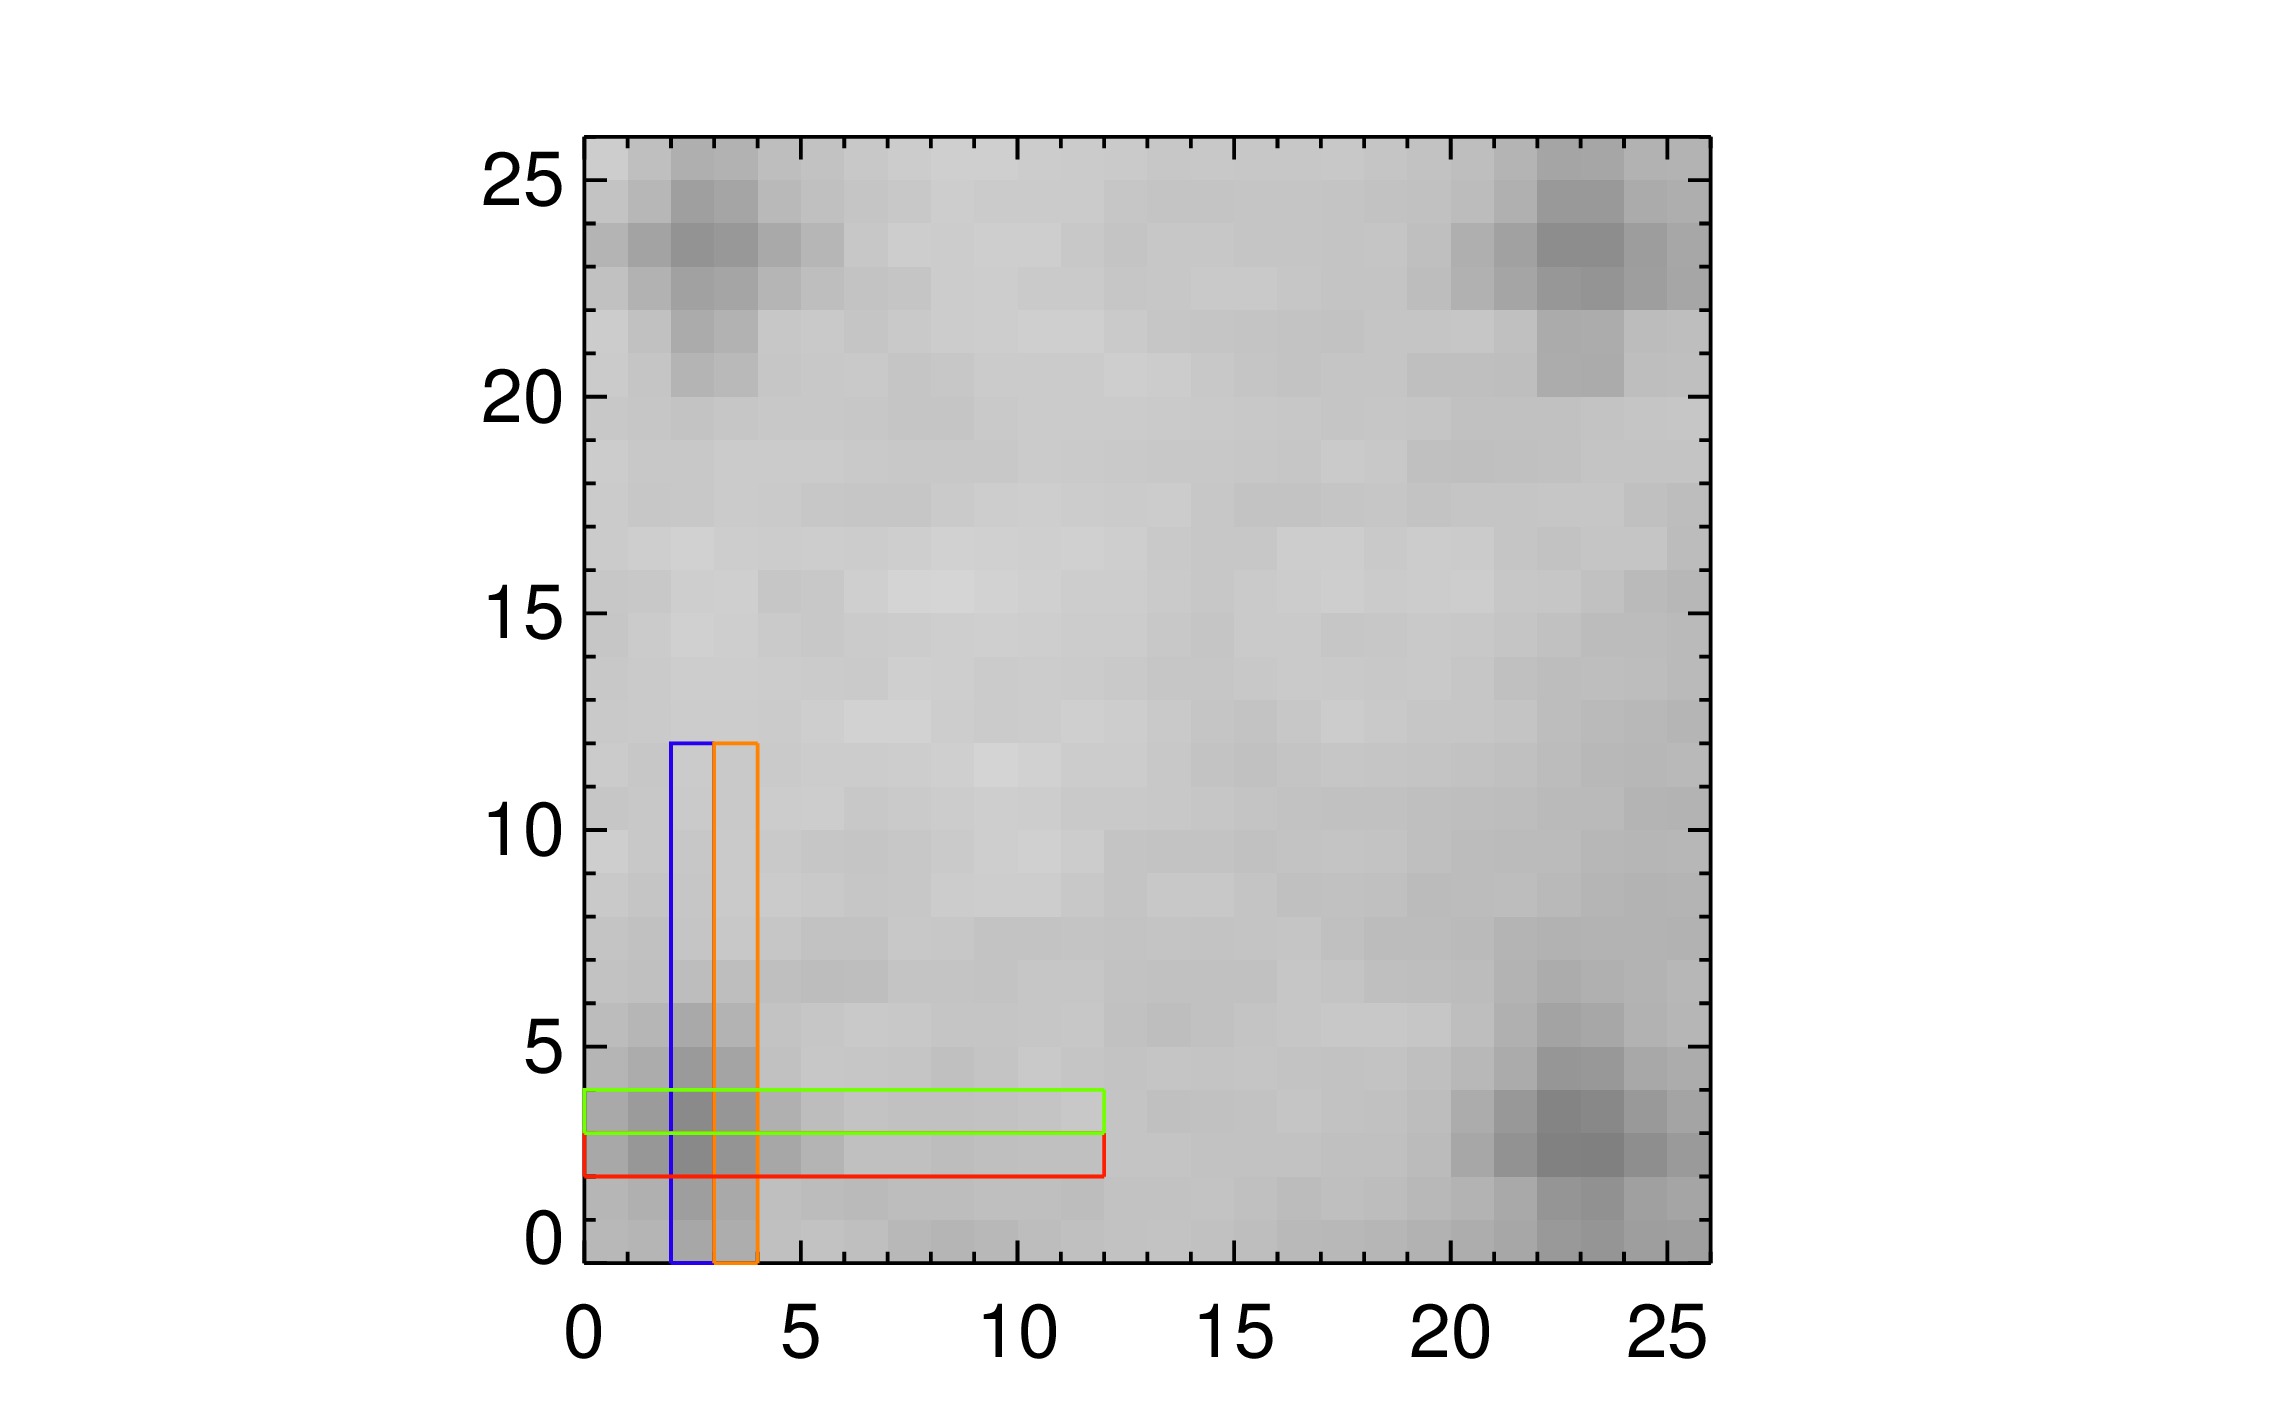
\includegraphics[width=1.5\textwidth]{../plots_tables_images/datcrop_color.png}
%         \caption{Where we are looking exactly. Figure \ref{firstone} corresponds to the red bar. It doesn't say anywhere in the plots but you'll have to trust me on this.}
%     \end{subfigure}
%     \caption{The cropped image we will be looking at}
%     \label{datcrop}
% \end{figure}

\begin{figure}[!ht]
    \ffigbox[][\FBheight]{%
    \begin{subfloatrow}[2]%
        \ffigbox[\FBwidth]%
       {%
       
\includegraphics[width=.5\textwidth]{../plots_tables_images/datcrop.png}%
       }%
       {%
       \caption{The cropped image we examine. I've purposely cropped it to be on the edge of all 4 fiducials to make analyzing the border pixels easier.}%
       }%
        \ffigbox[\Xhsize]%
       {%
       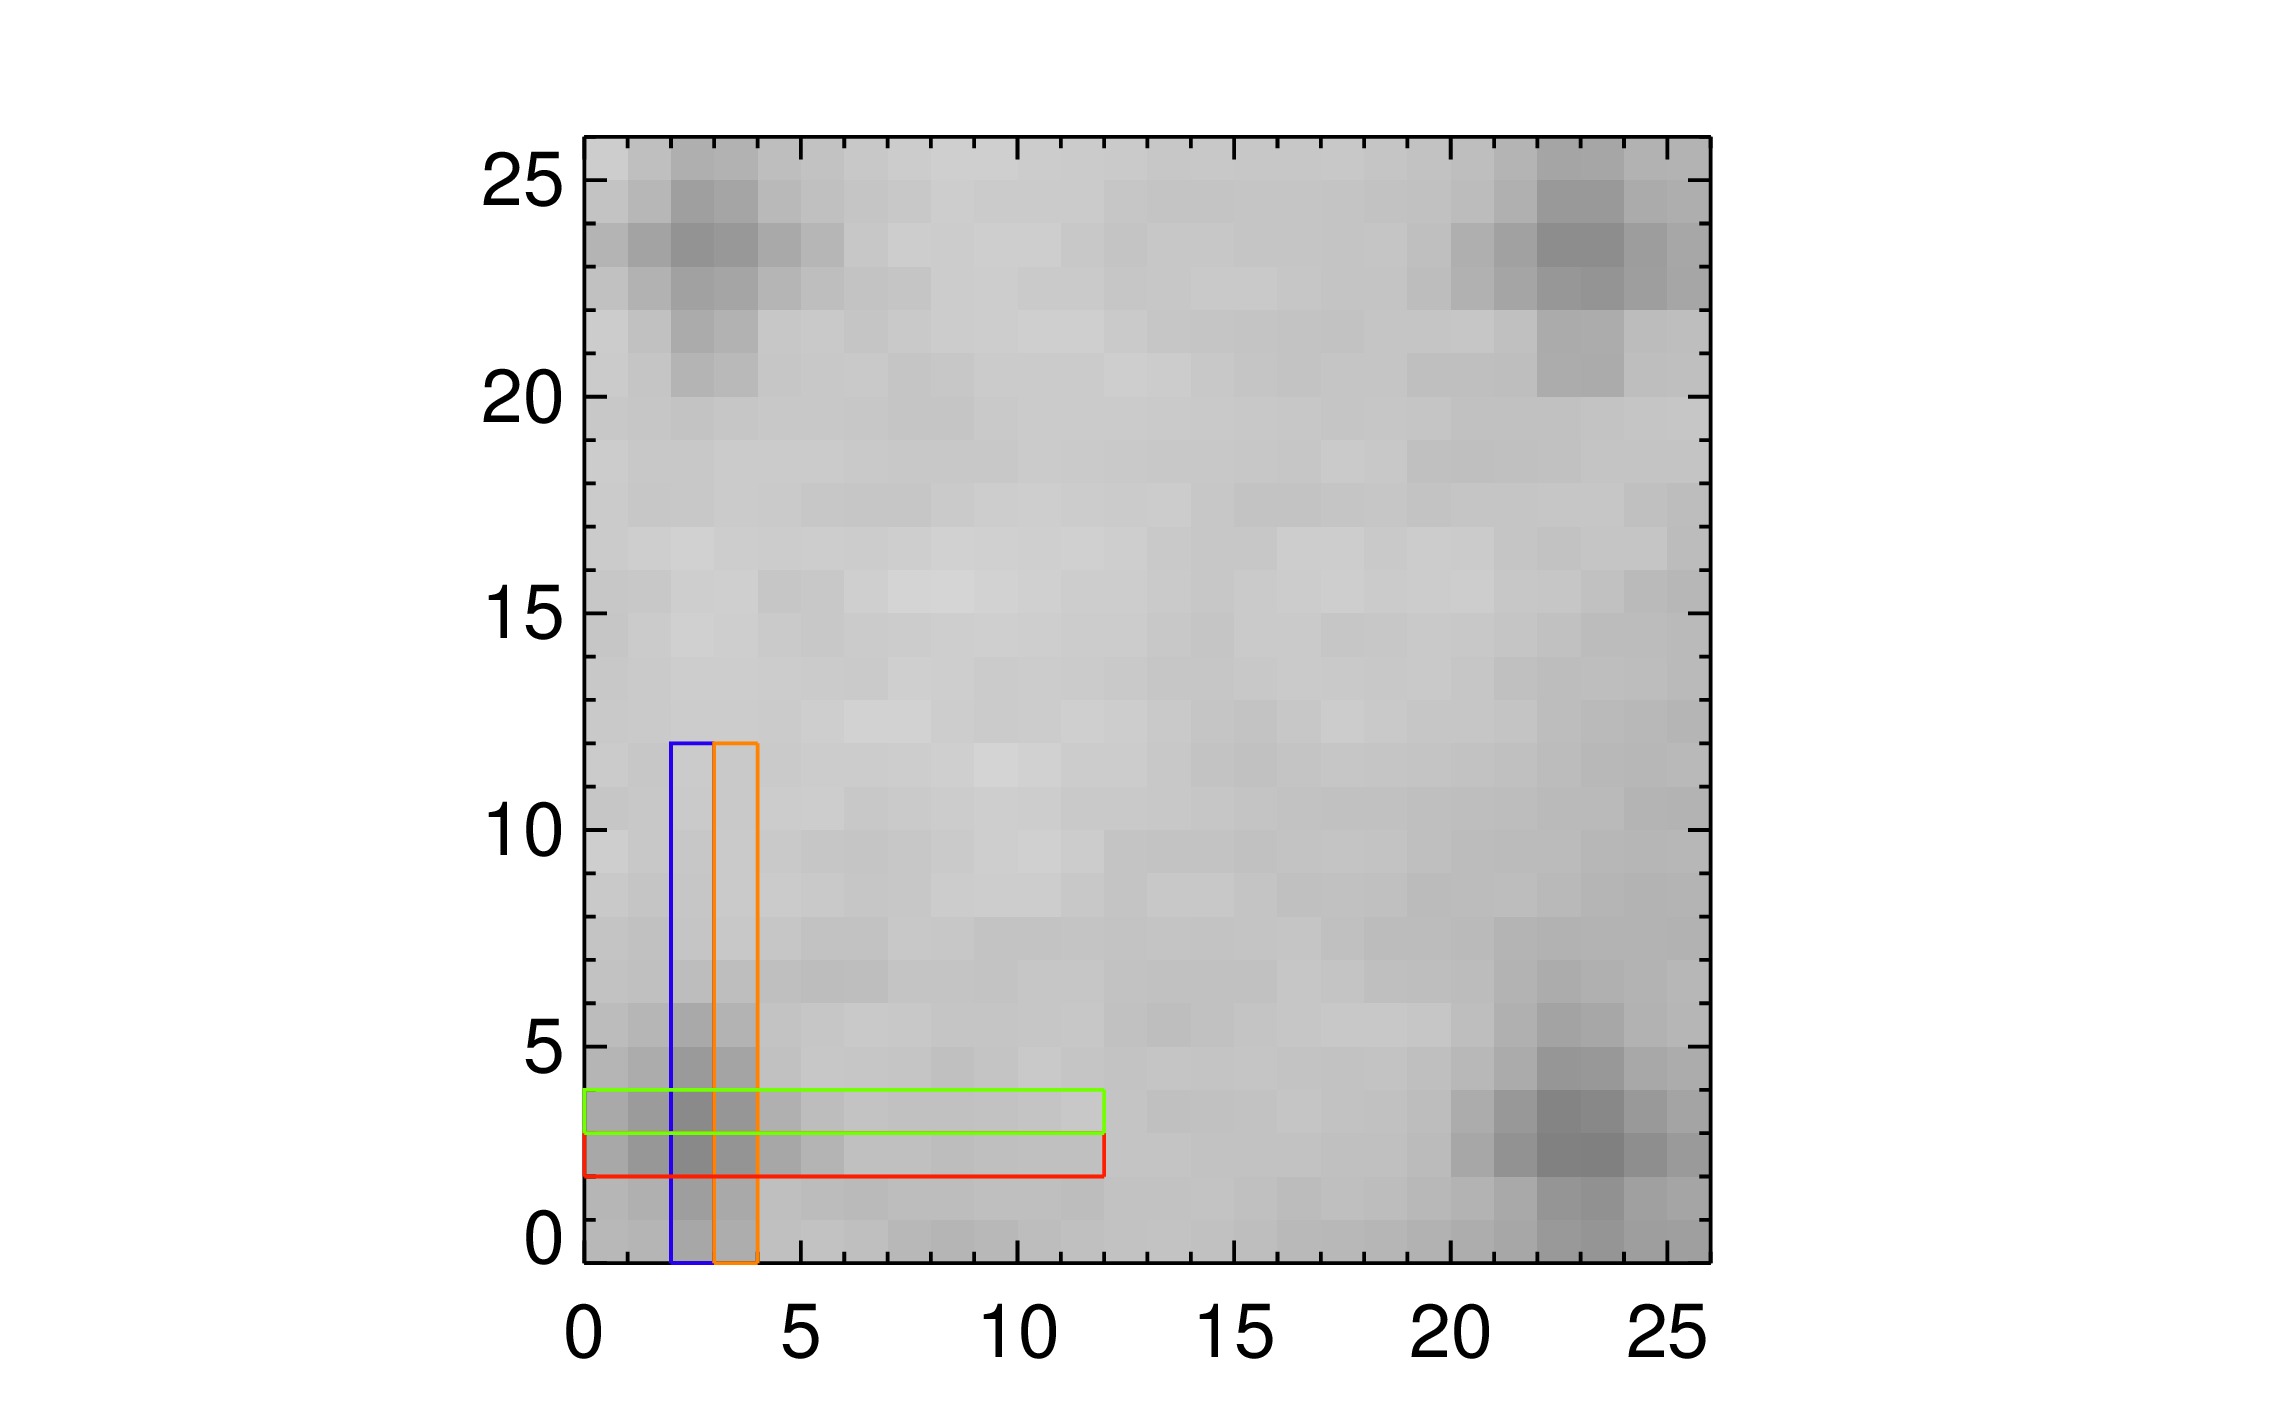
\includegraphics[width=.5\textwidth]{../plots_tables_images/datcrop_color.png}%
       }%
       {%
       \caption{Where we are looking exactly. Figure \ref{firstone} corresponds to the red bar. It doesn't say anywhere in the plots but you'll have to trust me on this.}%
       \label{datcrop}%
       }
    \end{subfloatrow}}{\caption{The cropped image we will be looking at}}%
\end{figure}

% section introduction (end)

\section{Fiducial Spectra} % (fold)
\label{sec:fiducial_spectra}

% \begin{figure}[!h]
%     \centering 
%     \hspace{-1.0in}
%     \begin{subfigure}[b]{.4\linewidth}
%         \centering
%         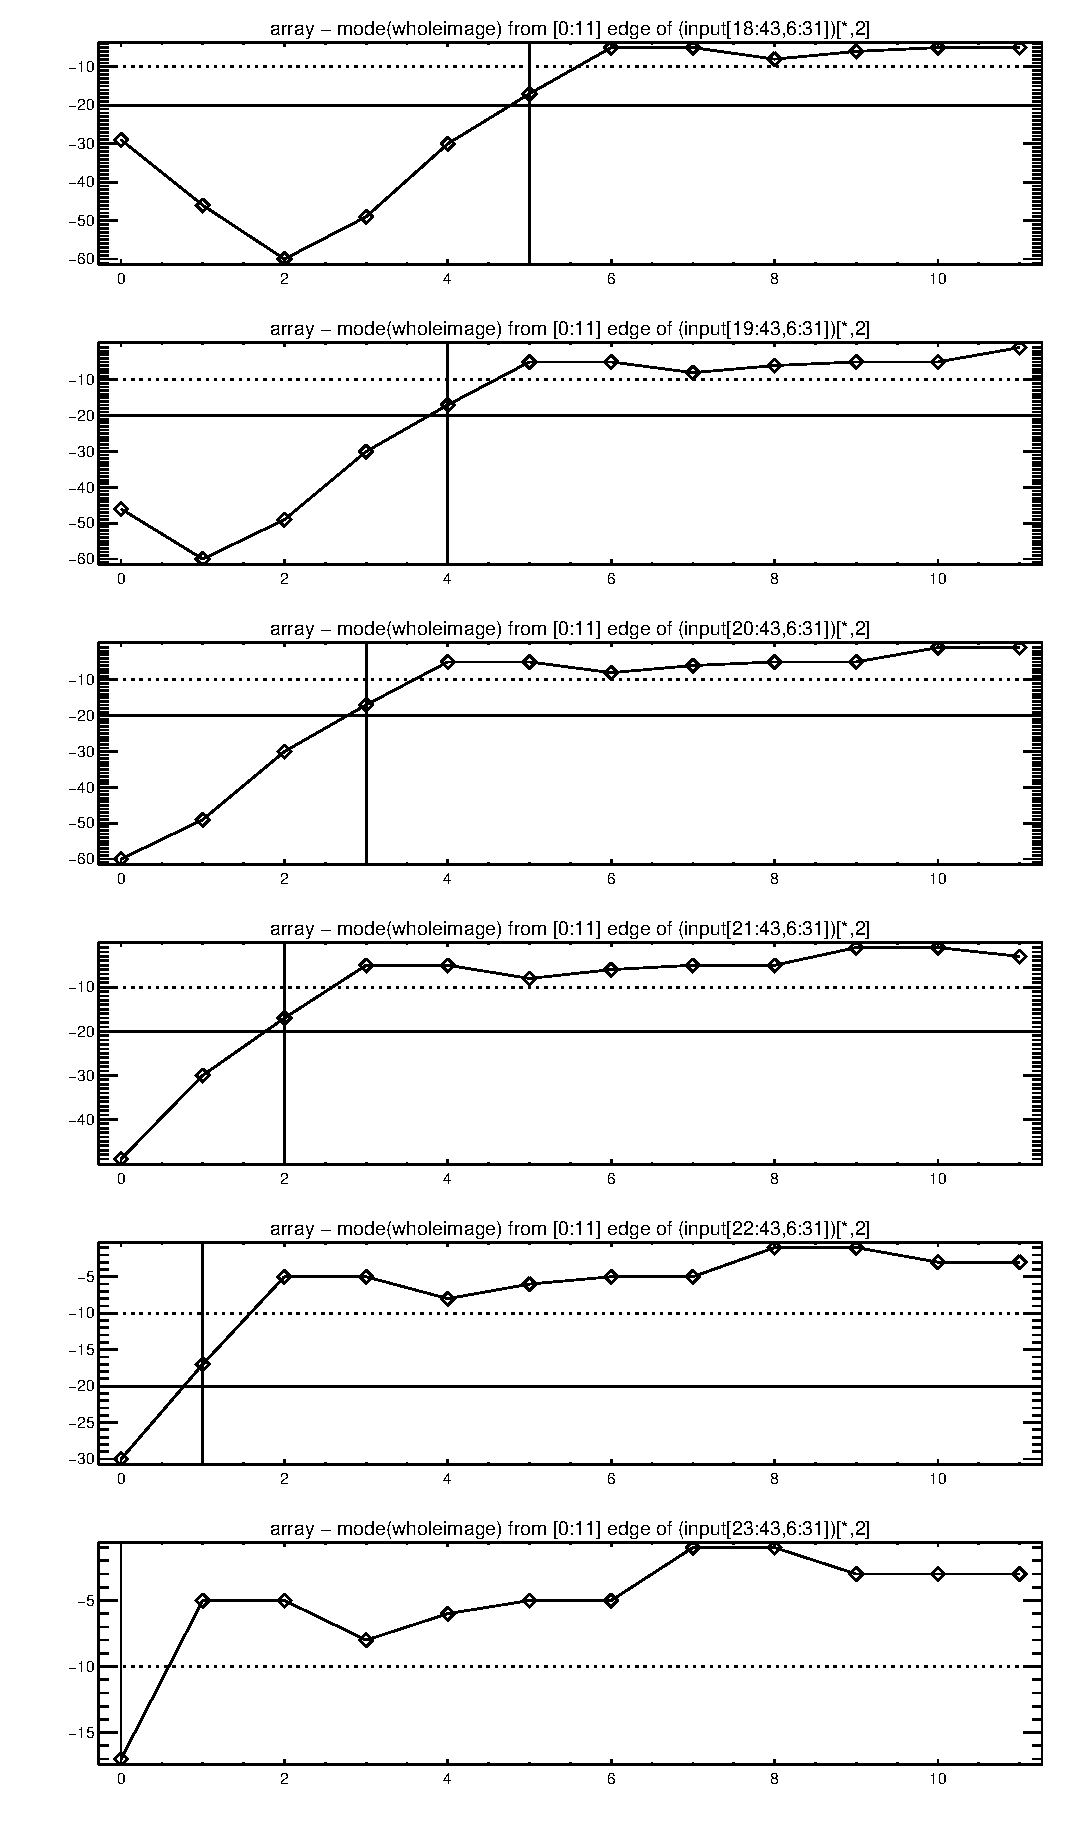
\includegraphics[width=1.4\textwidth]{../plots_tables_images/botleft0.eps} 
%         \caption{Ignore the title, the only relevant information there is the [0:11]. The part with input is so wrong. The solid line is at -20 and the dotted line is at -10. The vertical line represents the rightmost edge of the fiducial. In this case, the red bar in it's current position corresponds to the top-most plot here. As we shift the red bar 1 pixel at a time to the right, the fiducial gets more and more cut off until eventually there are no pixels left in the region we are looking.}
%         \label{primeone}
%     \end{subfigure}
%     \hspace{1.0in}
%     \begin{subfigure}[b]{.4\linewidth}
%         \centering
%         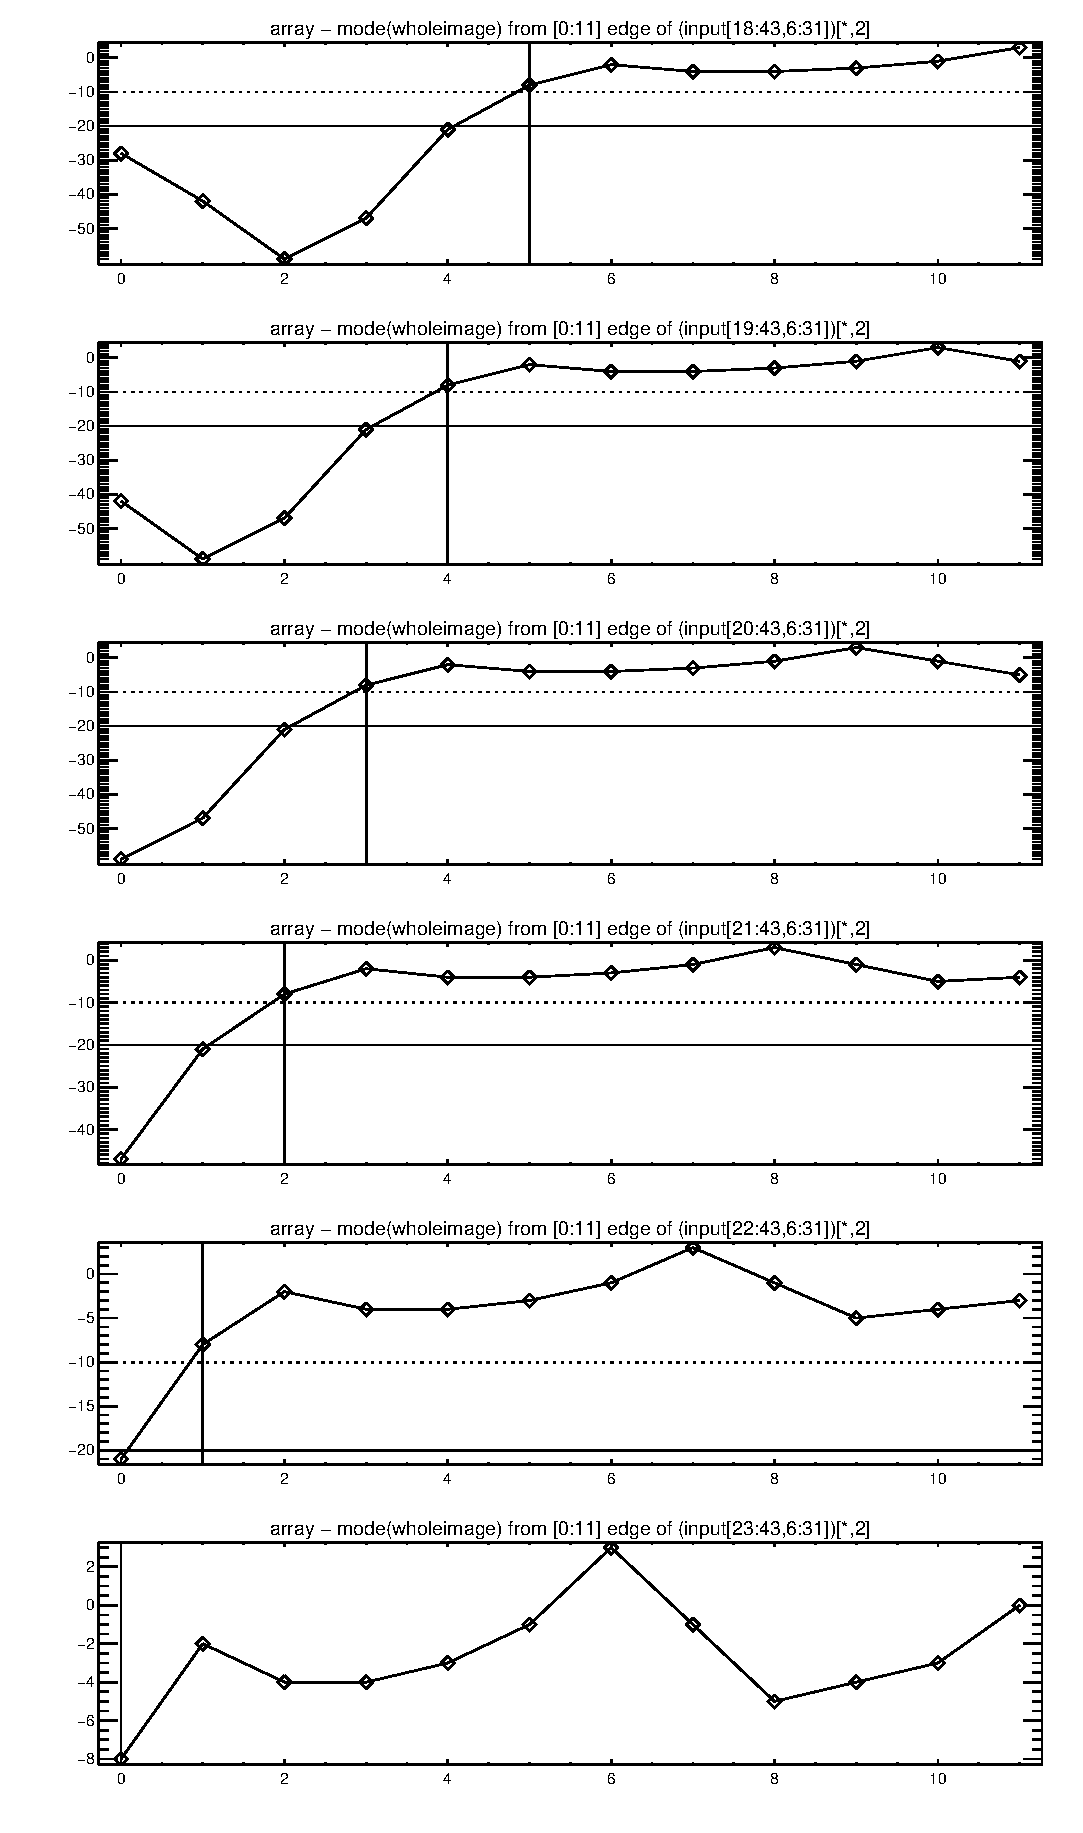
\includegraphics[width=1.4\textwidth]{../plots_tables_images/botleft1.eps} 
%         \caption{The green bar, same deal, moving left. Already we see that the threshold of -20 which worked well for the previous slice falls a bit short on the adjacent row of pixels.\\ \\ \\ \\ \\ \\ \\}
%     \end{subfigure}
%     \caption{Fiducial values along the red and green rows}
%     \label{firstone}
% \end{figure}

\begin{figure}[!ht]
    \ffigbox[][\FBheight]{%
    \begin{subfloatrow}[2]%
        \ffigbox[\FBwidth]%
       {%
       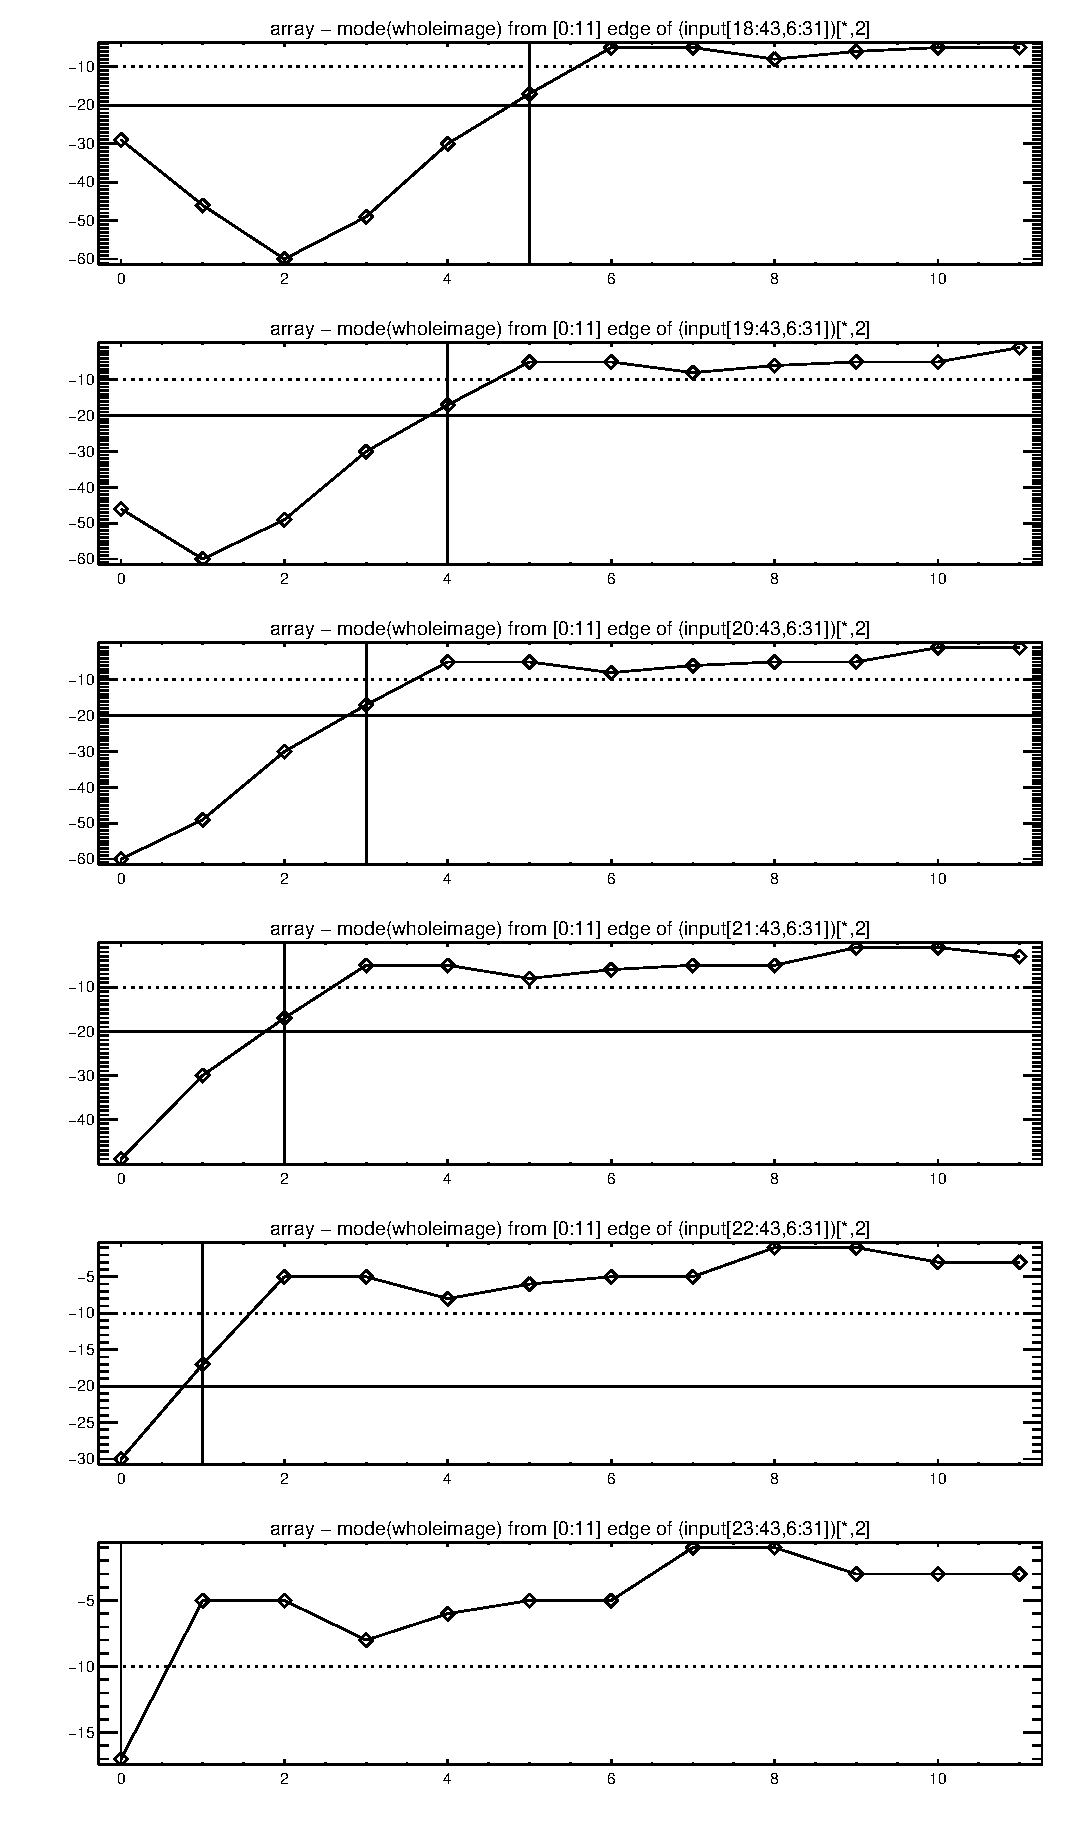
\includegraphics[width=.5\textwidth]{../plots_tables_images/botleft0.eps}%
       }%
       {%
       \caption{Ignore the title, the only relevant information there is the [0:11]. The part with input is so wrong. The solid line is at -20 and the dotted line is at -10. The vertical line represents the rightmost edge of the fiducial. In this case, the red bar in it's current position corresponds to the top-most plot here. As we shift the red bar 1 pixel at a time to the right, the fiducial gets more and more cut off until eventually there are no pixels left in the region we are looking.}\label{primeone}%
       }%
        \ffigbox[\Xhsize]%
       {%
       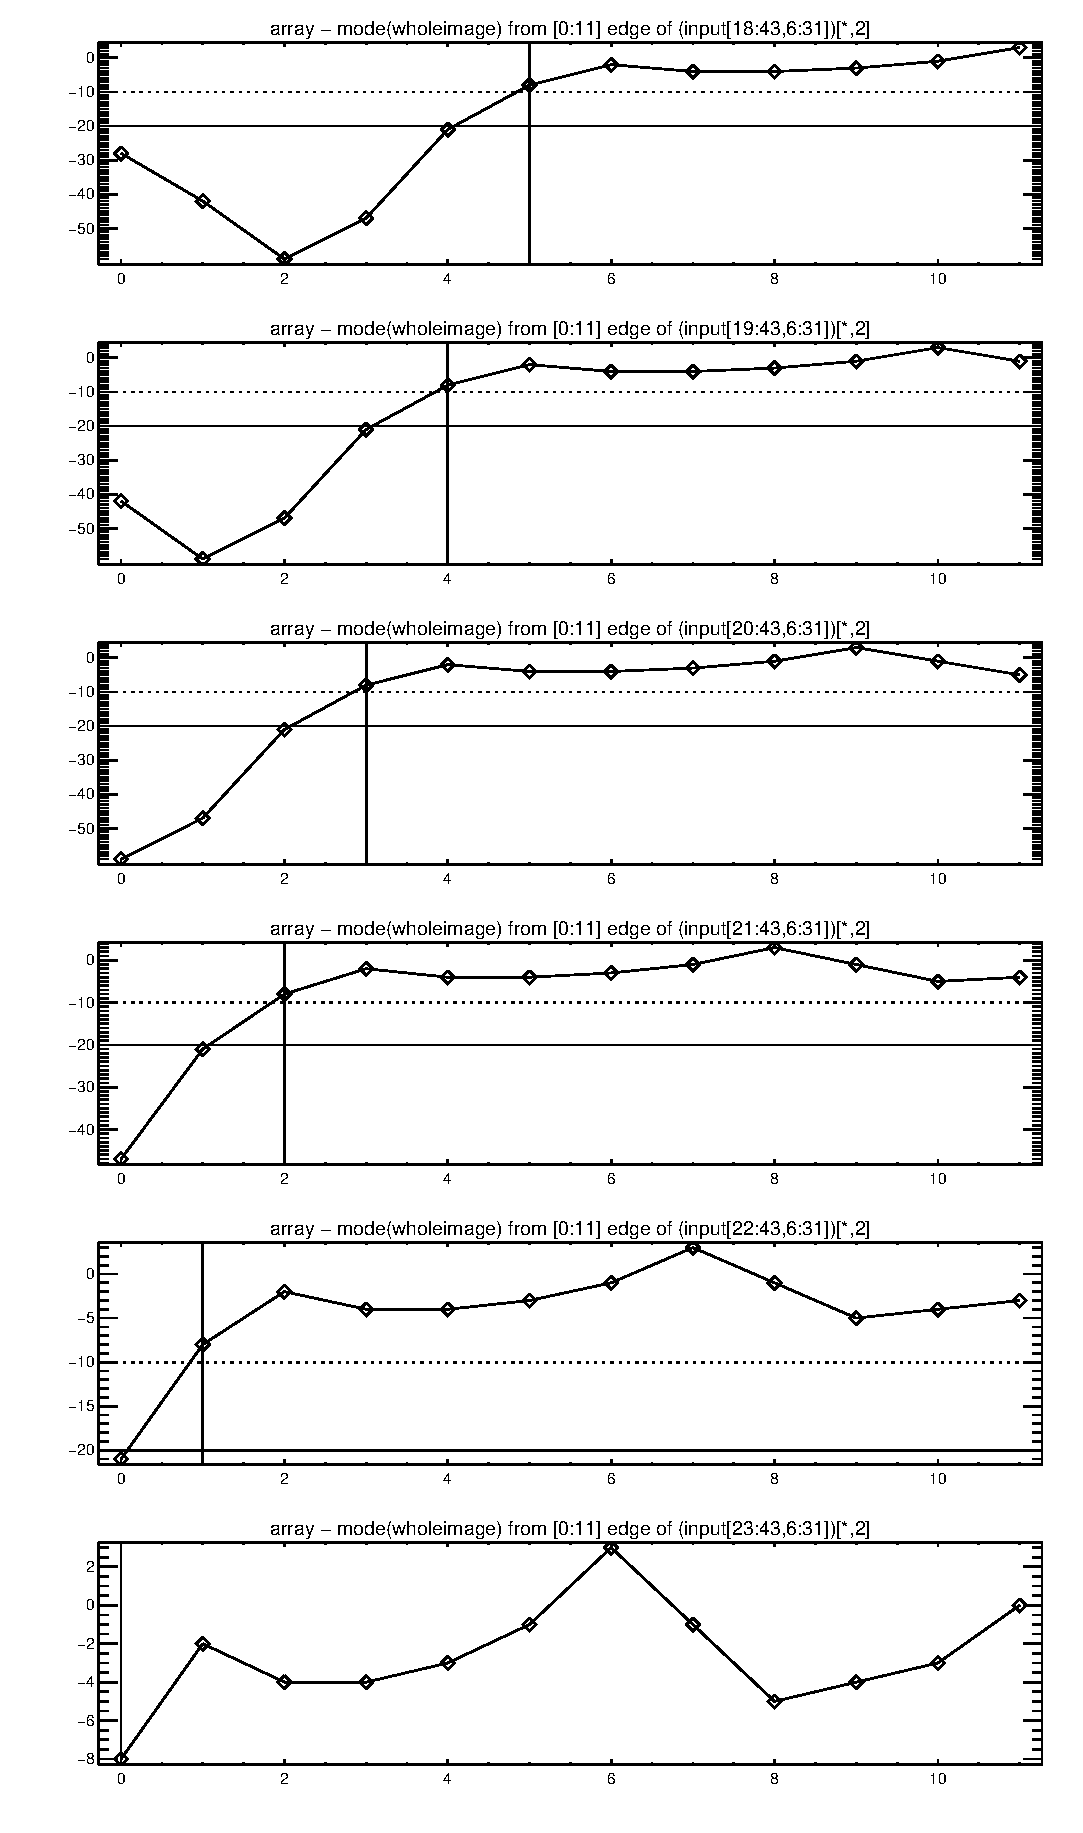
\includegraphics[width=.5\textwidth]{../plots_tables_images/botleft1.eps}%
       }%
       {%
       \caption{The green bar, same deal, moving left. Already we see that the threshold of -20 which worked well for the previous slice falls a bit short on the adjacent row of pixels.}%
       }%
    \end{subfloatrow}}{\caption{Fiducial values along the red and green rows}\label{firstone}}%
\end{figure}


We see in Figure \ref{primeone} that if we look at the last pixels on the edge of the border, subtracting the mode of the cropped image gives us a threshold of about $-20$ with which we can use to identify the fiducial. If we count how many pixels are below the -20 threshold, we can more or less retrieve the number of pixels cut off by the edge. 

% \begin{figure}[!h]
%     \centering 
%     \hspace{-1.0in}
%     \begin{subfigure}[b]{.4\linewidth}
%         \centering
%         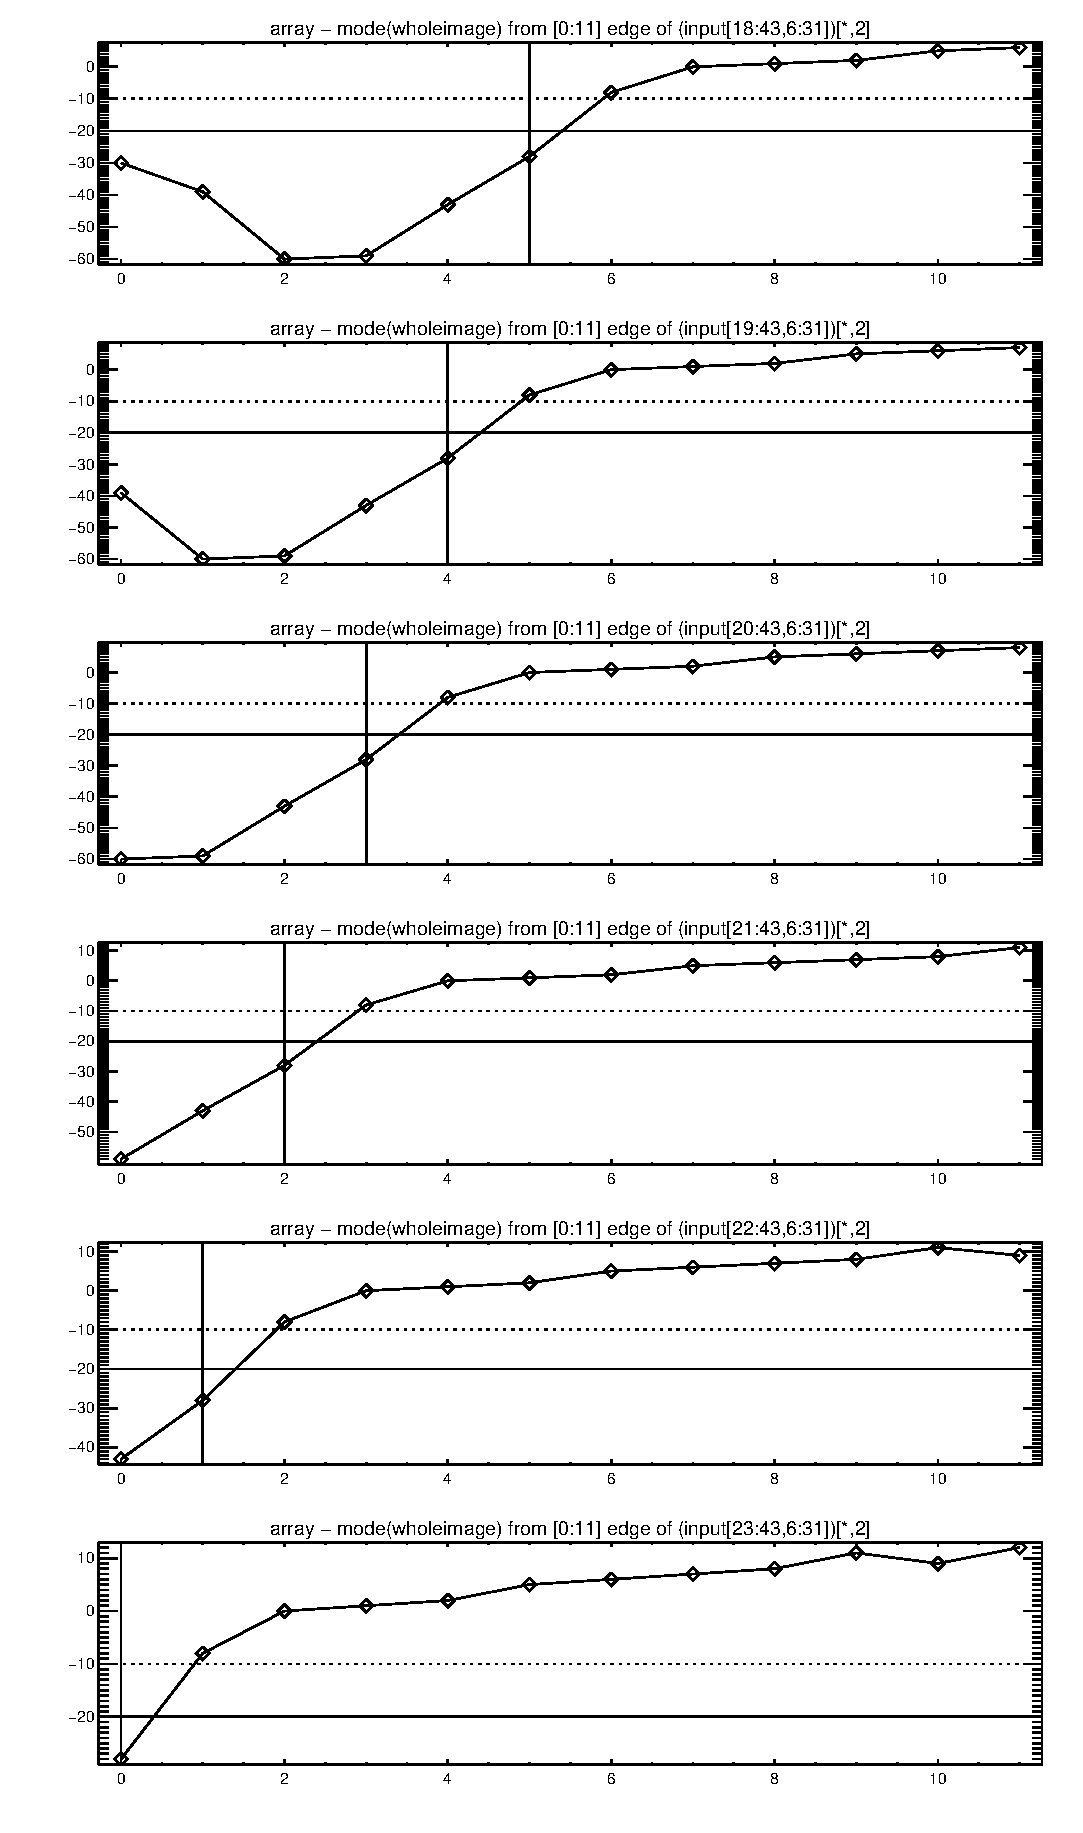
\includegraphics[width=1.4\textwidth]{../plots_tables_images/botleft2.eps} 
%         \caption{The blue bar, now moving up. Here the threshold is more around -20. \\}
%     \end{subfigure}
%     \hspace{1.0in}
%     \begin{subfigure}[b]{.4\linewidth}
%         \centering
%         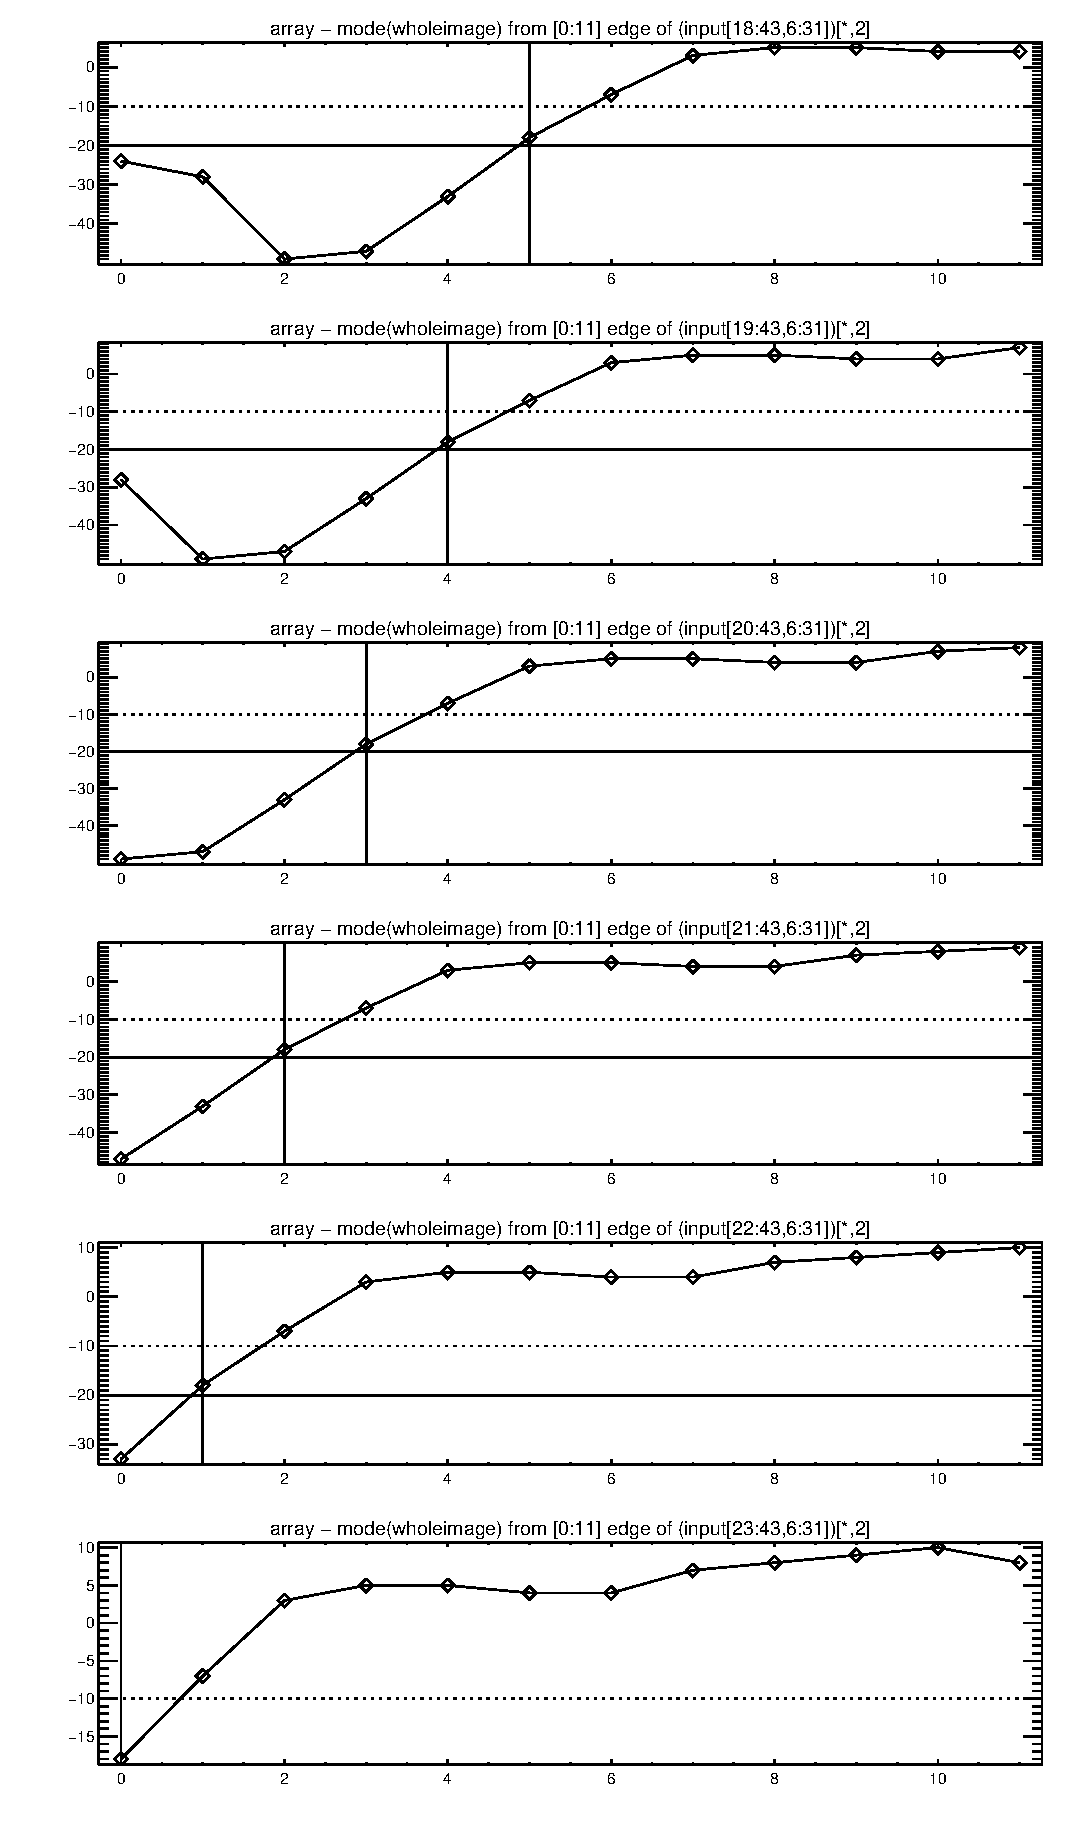
\includegraphics[width=1.4\textwidth]{../plots_tables_images/botleft3.eps} 
%         \caption{The orange bar, moving up as well. The threshold is consistent with the adjacent threshold of -20}
%     \end{subfigure}
%     \caption{Blue and Orange Columns}
%     \label{secondone}
% \end{figure}

\begin{figure}[!ht]
    \ffigbox[][\FBheight]{%
    \begin{subfloatrow}[2]%
        \ffigbox[\FBwidth]%
       {%
       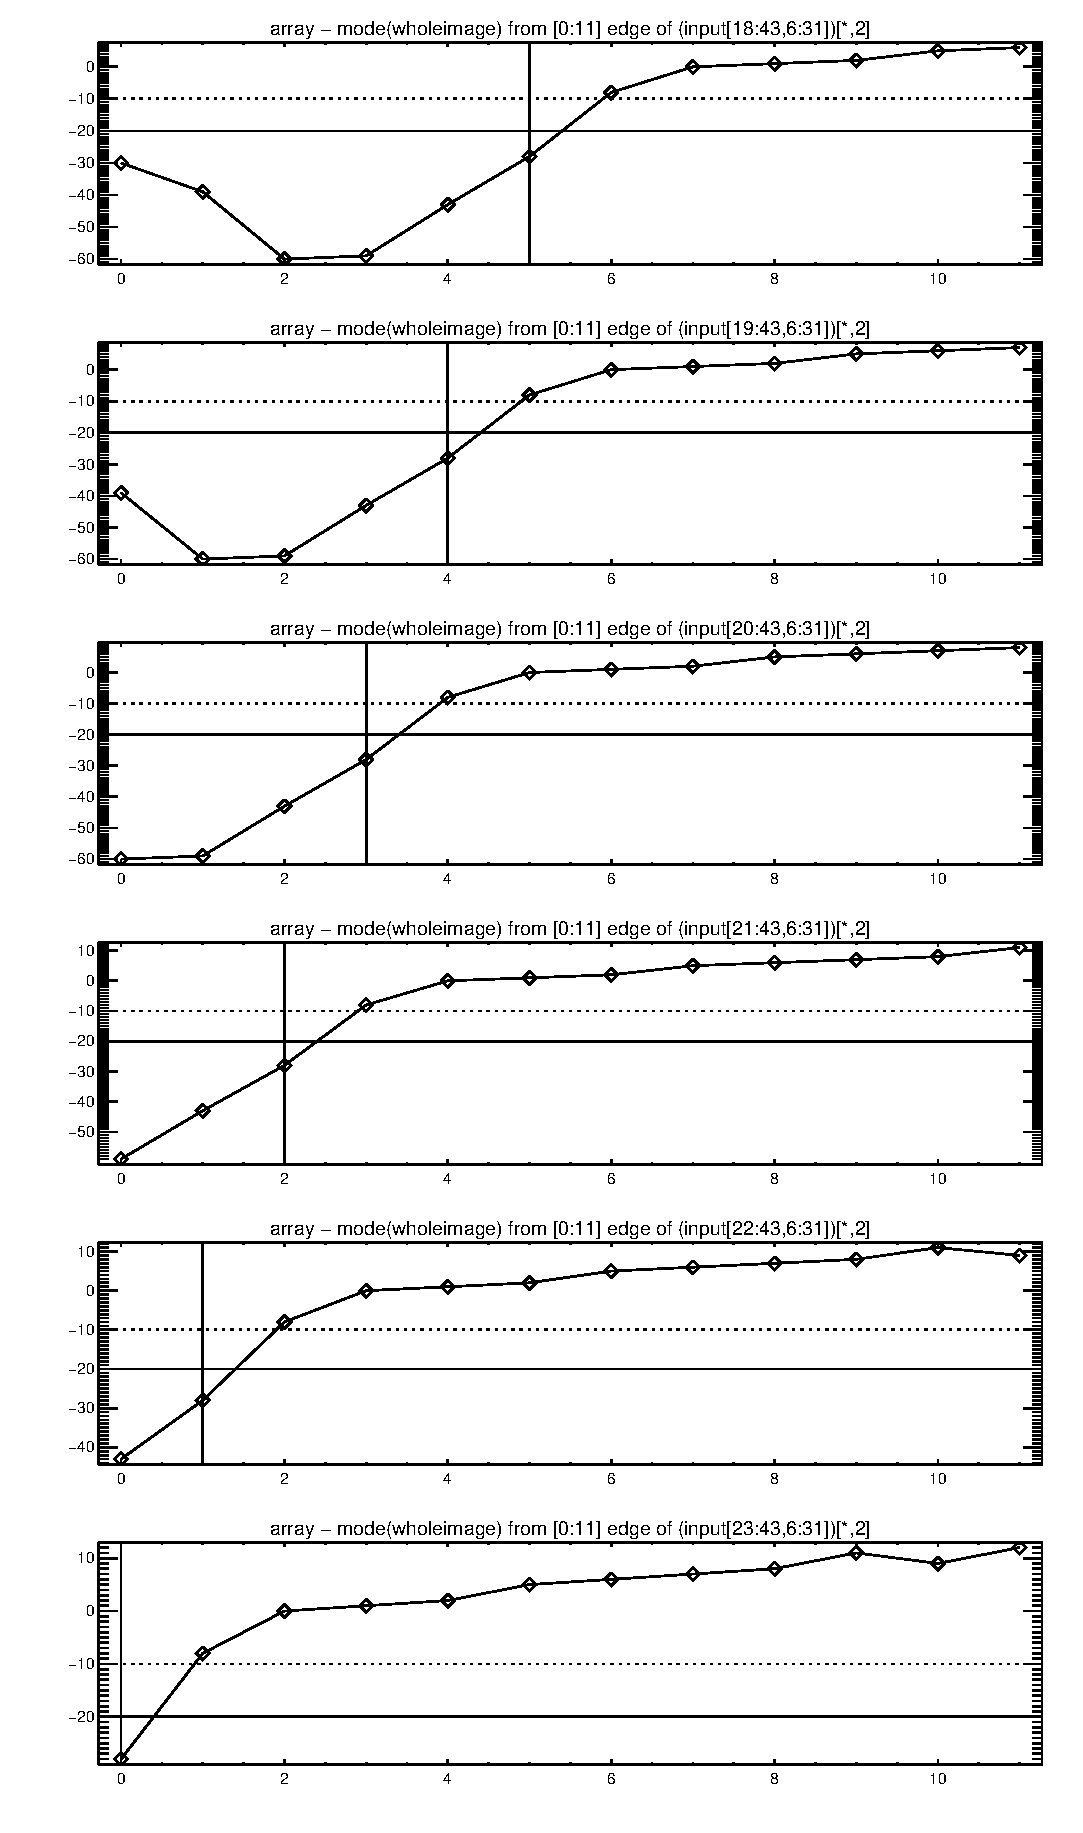
\includegraphics[width=.5\textwidth]{../plots_tables_images/botleft2.eps}%
       }%
       {%
       \caption{The blue bar, now moving up. Here the threshold is more around -20.}%
       }%
        \ffigbox[\Xhsize]%
       {%
       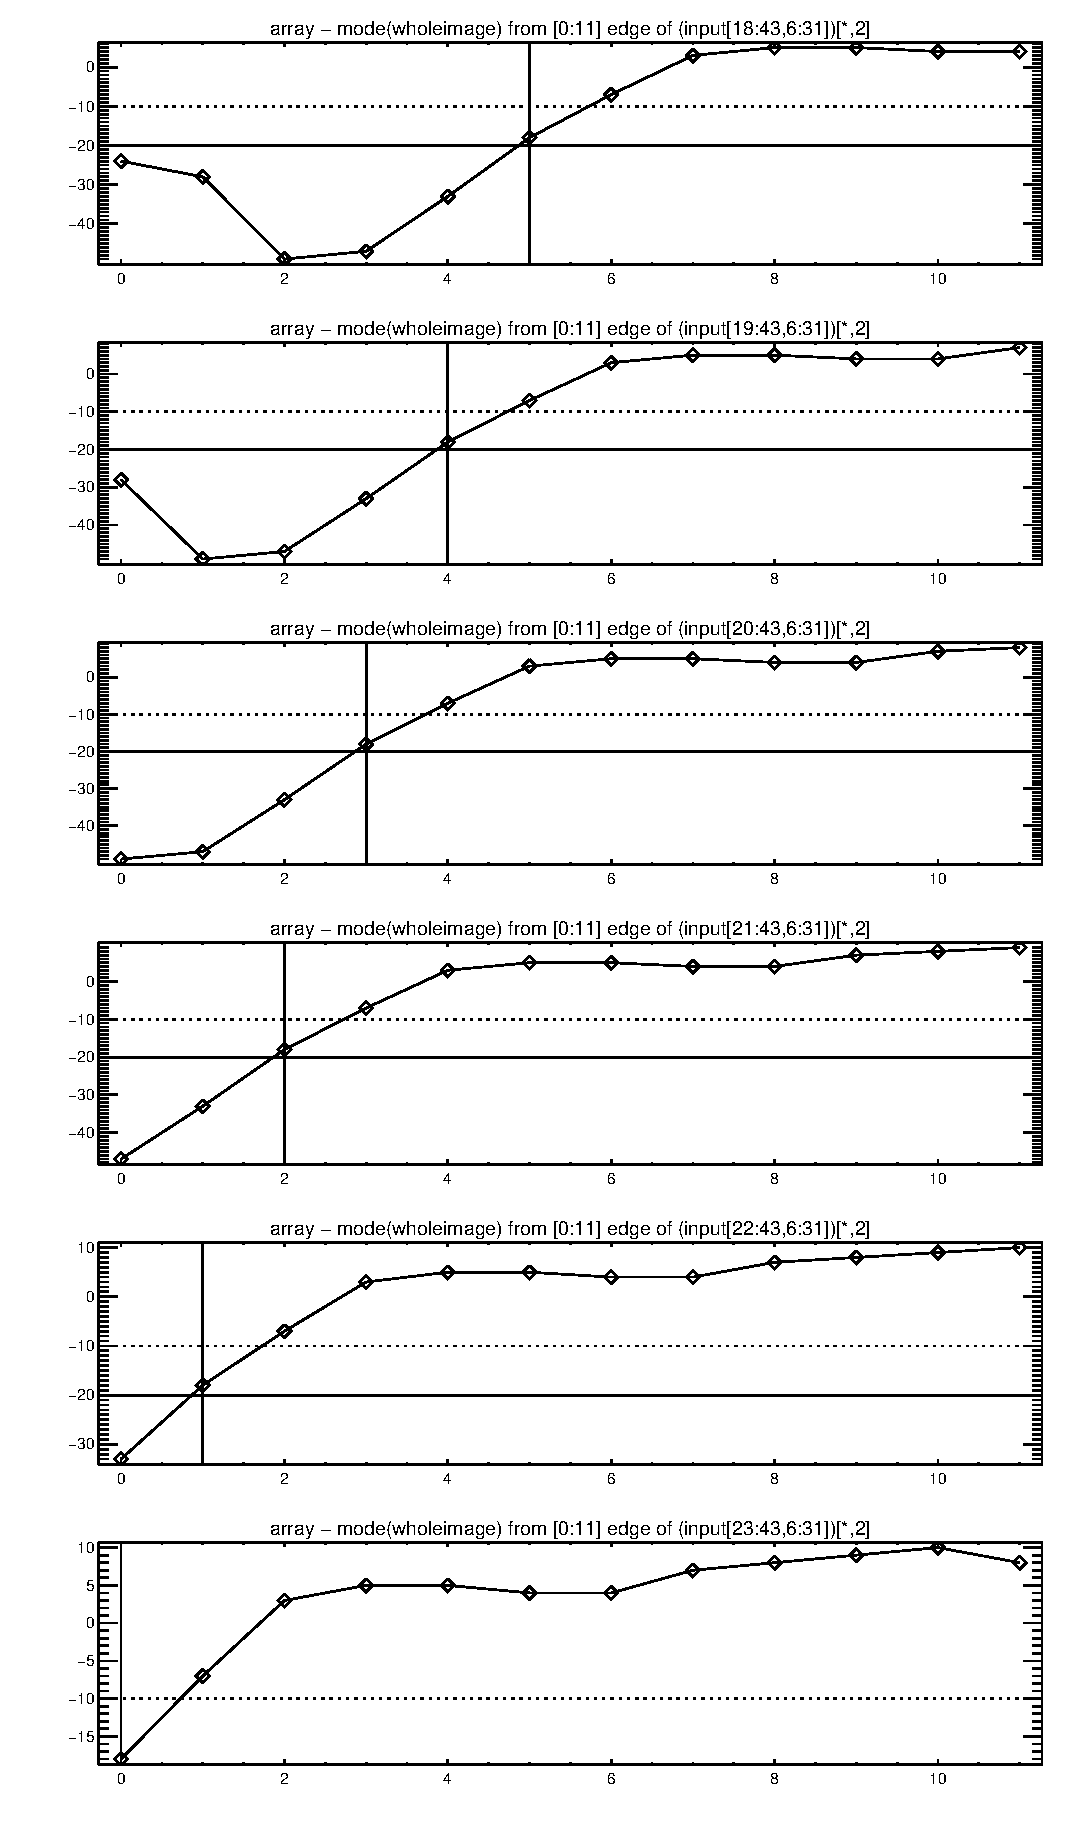
\includegraphics[width=.5\textwidth]{../plots_tables_images/botleft3.eps}%
       }%
       {%
       \caption{The orange bar, moving up as well. The threshold is consistent with the adjacent threshold of -20.}%
       }%
    \end{subfloatrow}}{\caption{Blue and Orange Columns}\label{secondone}}%
\end{figure}

% section fiducial_spectra (end)

\clearpage
\newpage

\section{Laying Down the Law (And a Lot of Plots)} % (fold)
\label{sec:laying_down_the_law_}


\begin{figure}[!ht]
    \ffigbox[][\FBheight]{%
    \begin{subfloatrow}[2]%
        \ffigbox[\FBwidth]%
       {%
       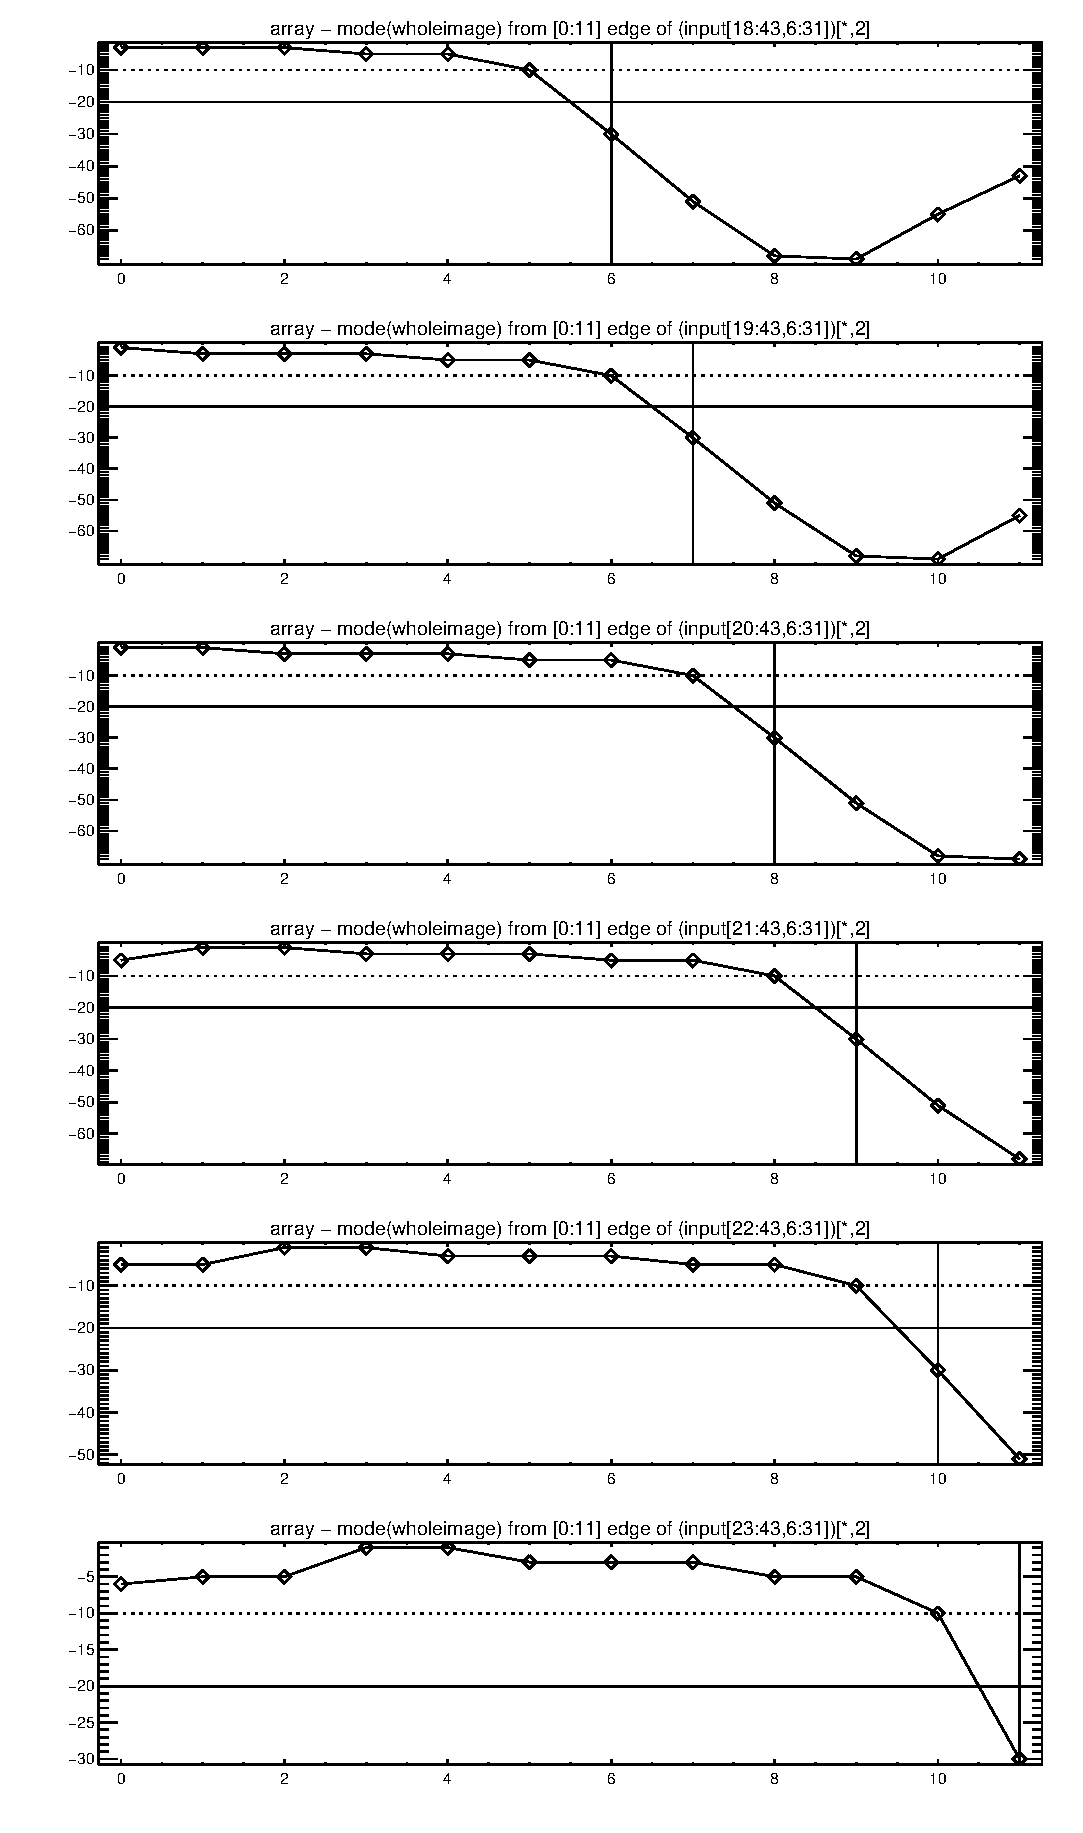
\includegraphics[width=.5\textwidth]{../plots_tables_images/botright0.eps}%
       }%
       {%
       \caption{Bottom right, bottom row}%
       }%
        \ffigbox[\Xhsize]%
       {%
       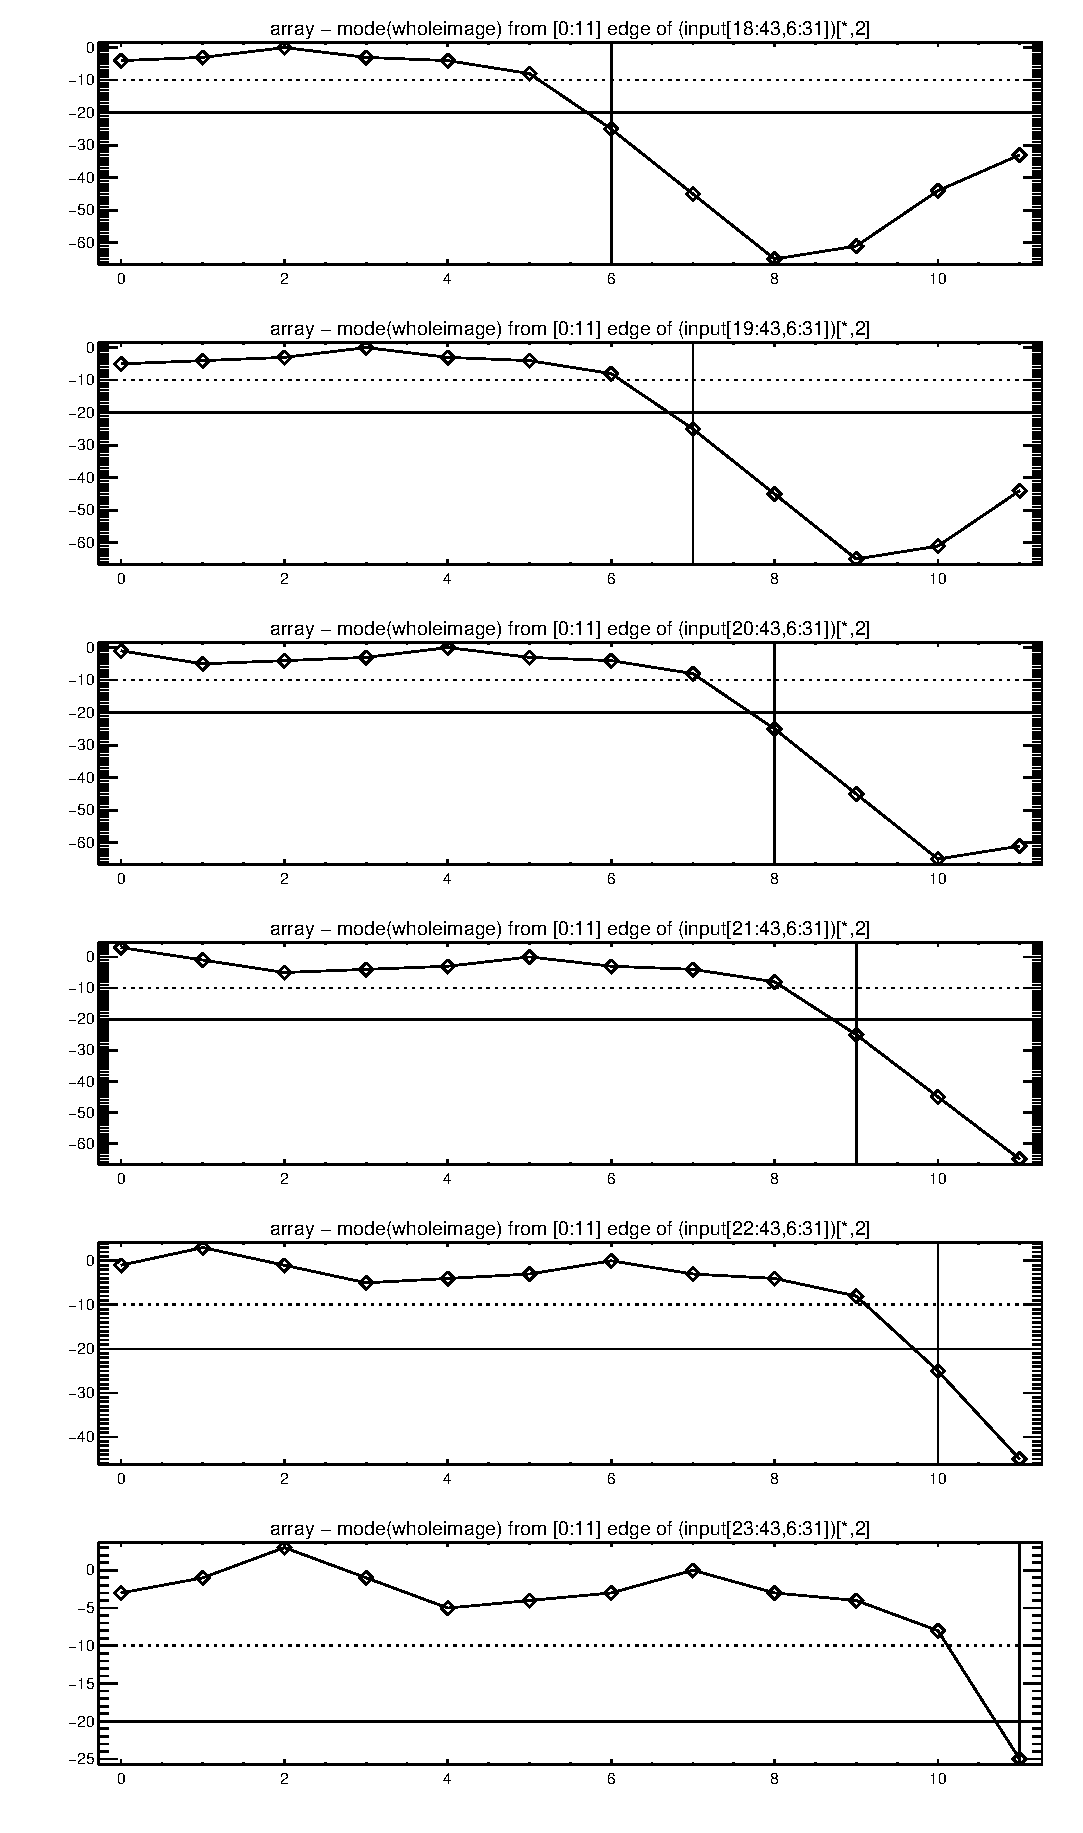
\includegraphics[width=.5\textwidth]{../plots_tables_images/botright1.eps}%
       }%
       {%
       \caption{Bottom right, top row}%
       }%
    \end{subfloatrow}}{\caption{}}%
\end{figure}

\begin{figure}[!ht]
    \ffigbox[][\FBheight]{%
    \begin{subfloatrow}[2]%
        \ffigbox[\FBwidth]%
       {%
       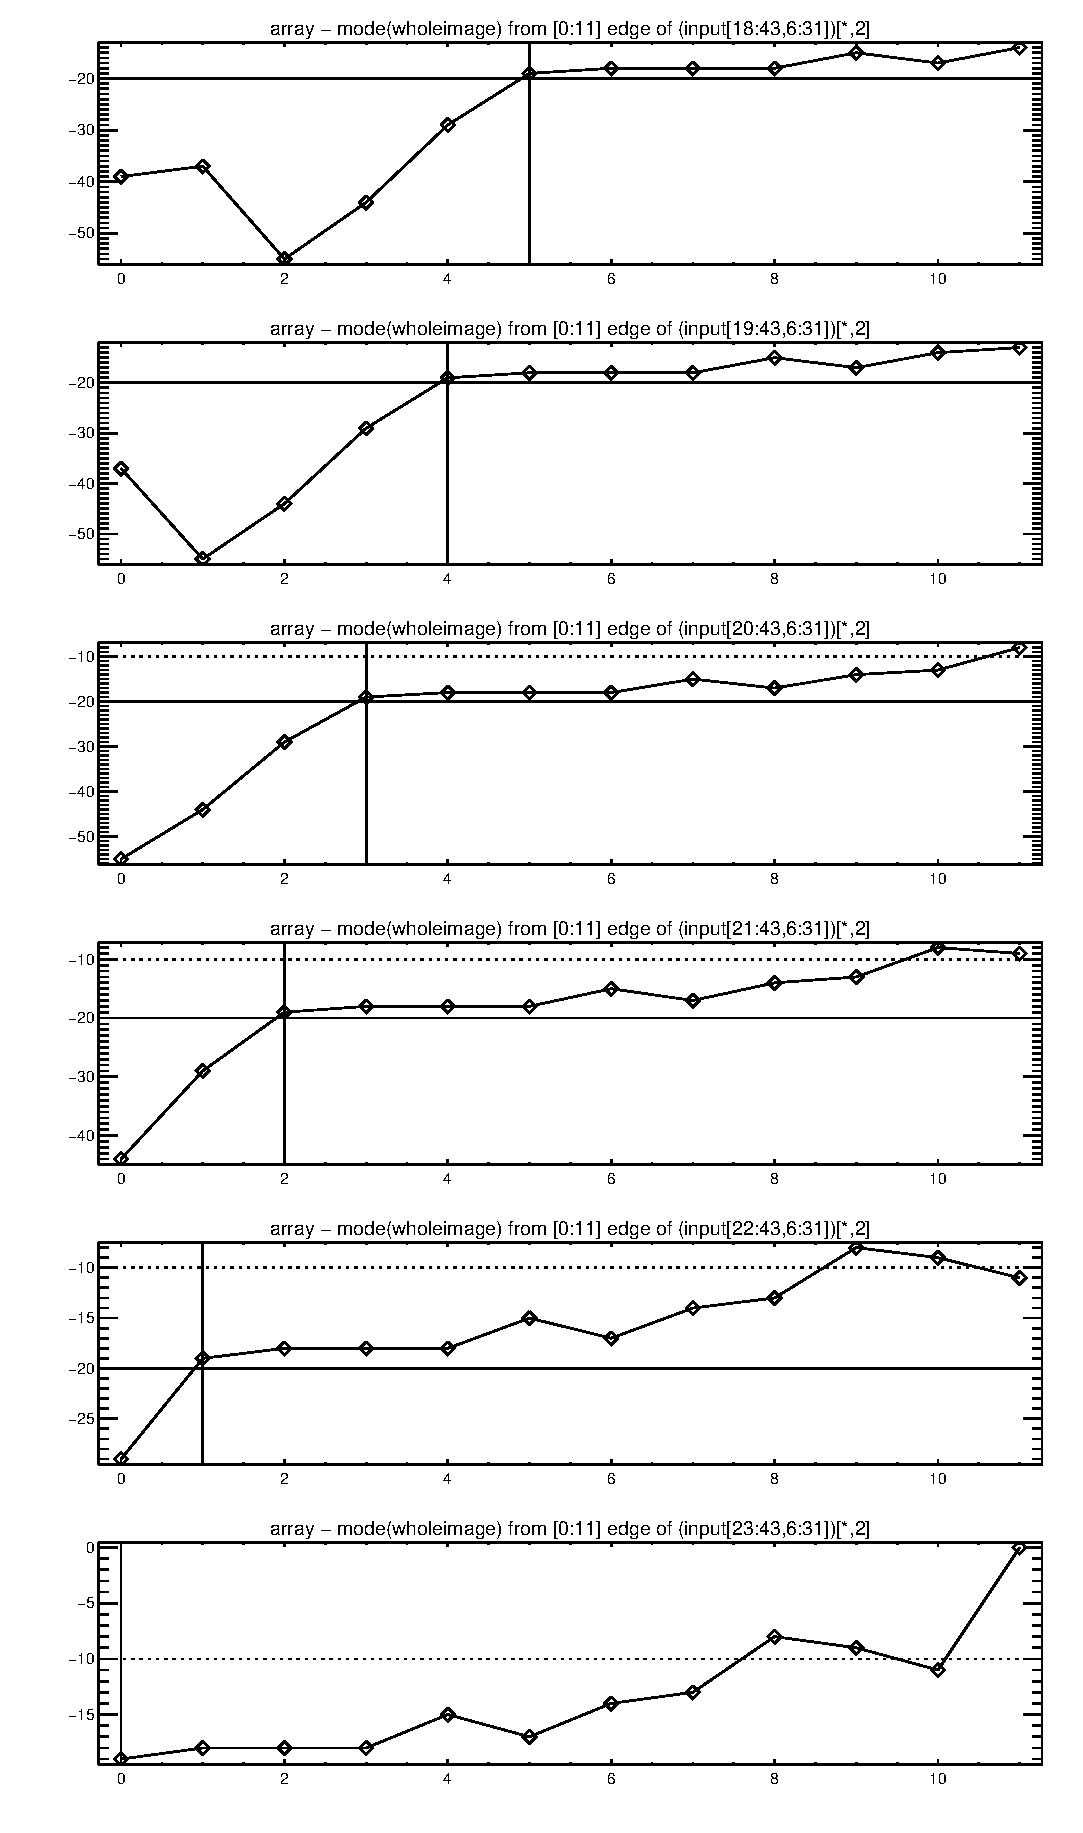
\includegraphics[width=.5\textwidth]{../plots_tables_images/botright2.eps}%
       }%
       {%
       \caption{Bottom right, right column}%
       }%
        \ffigbox[\Xhsize]%
       {%
       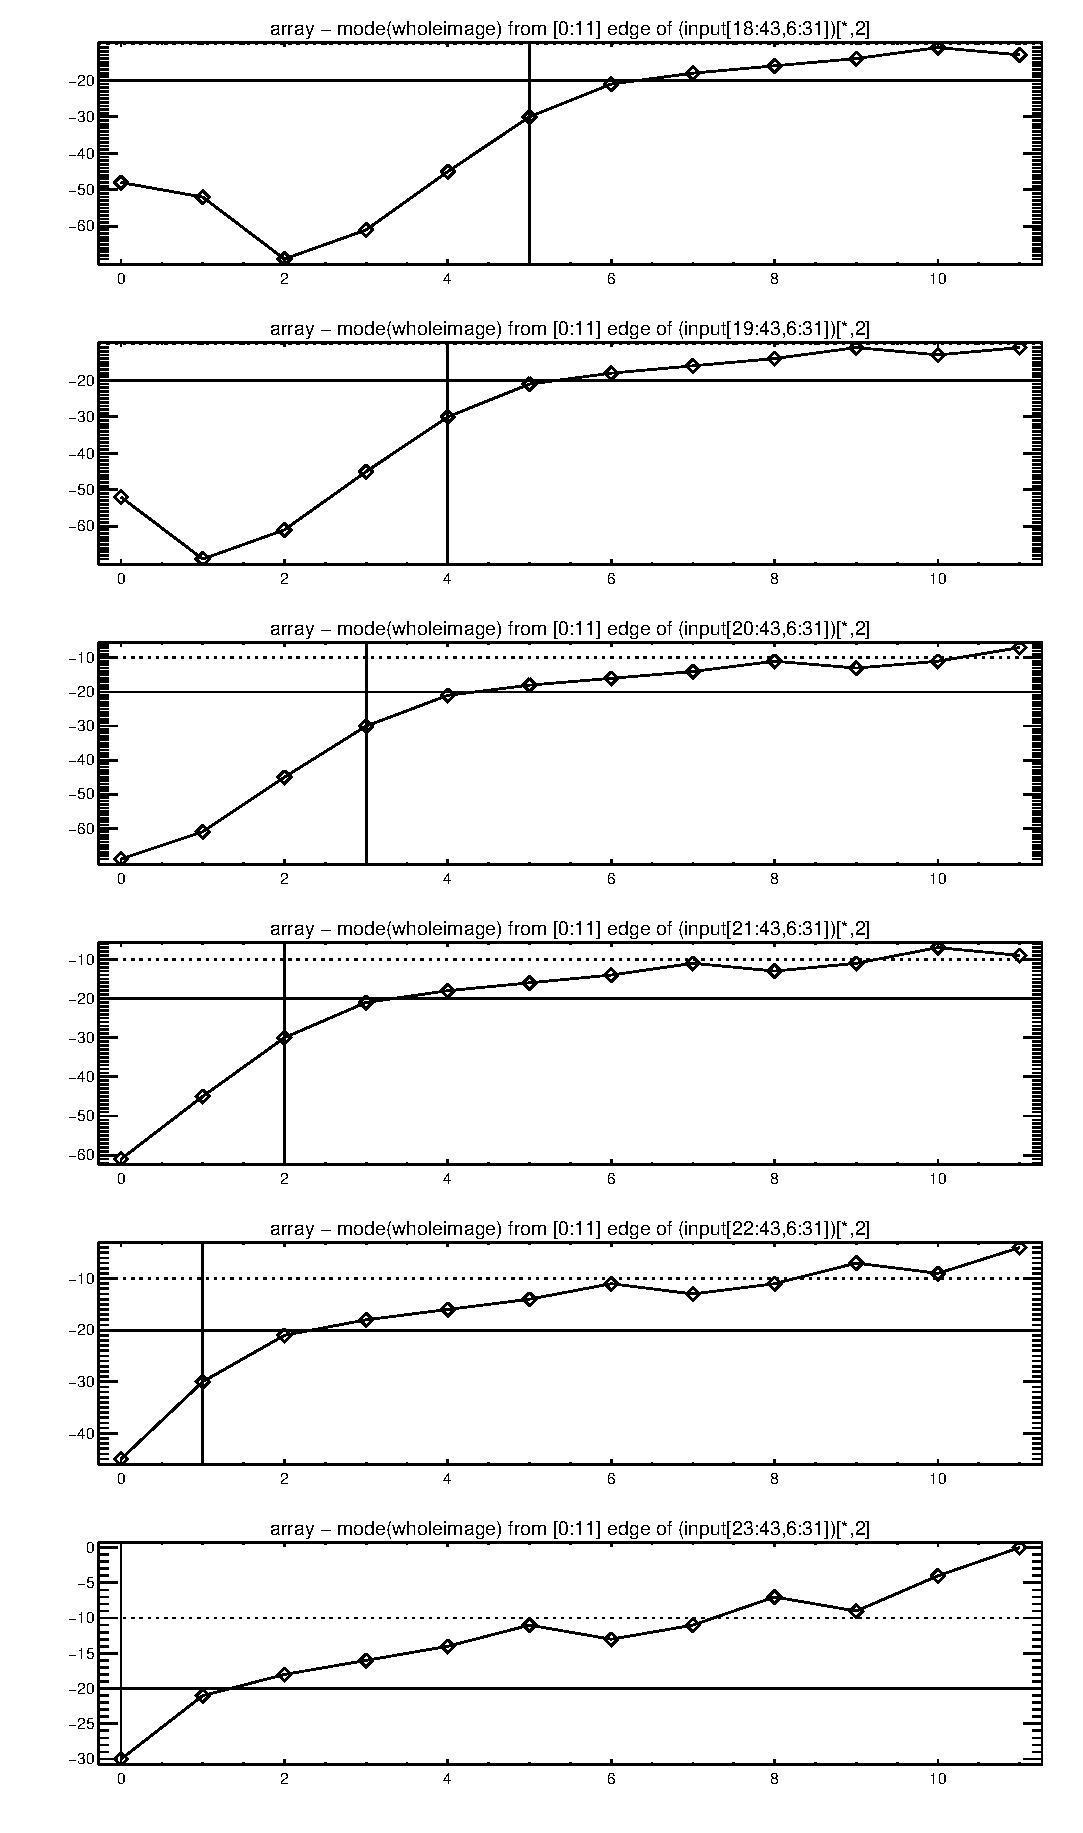
\includegraphics[width=.5\textwidth]{../plots_tables_images/botright3.eps}%
       }%
       {%
       \caption{Bottom right, left column}%
       }%
    \end{subfloatrow}}{\caption{}}%
\end{figure}

\begin{figure}[!ht]
    \ffigbox[][\FBheight]{%
    \begin{subfloatrow}[2]%
        \ffigbox[\FBwidth]%
       {%
       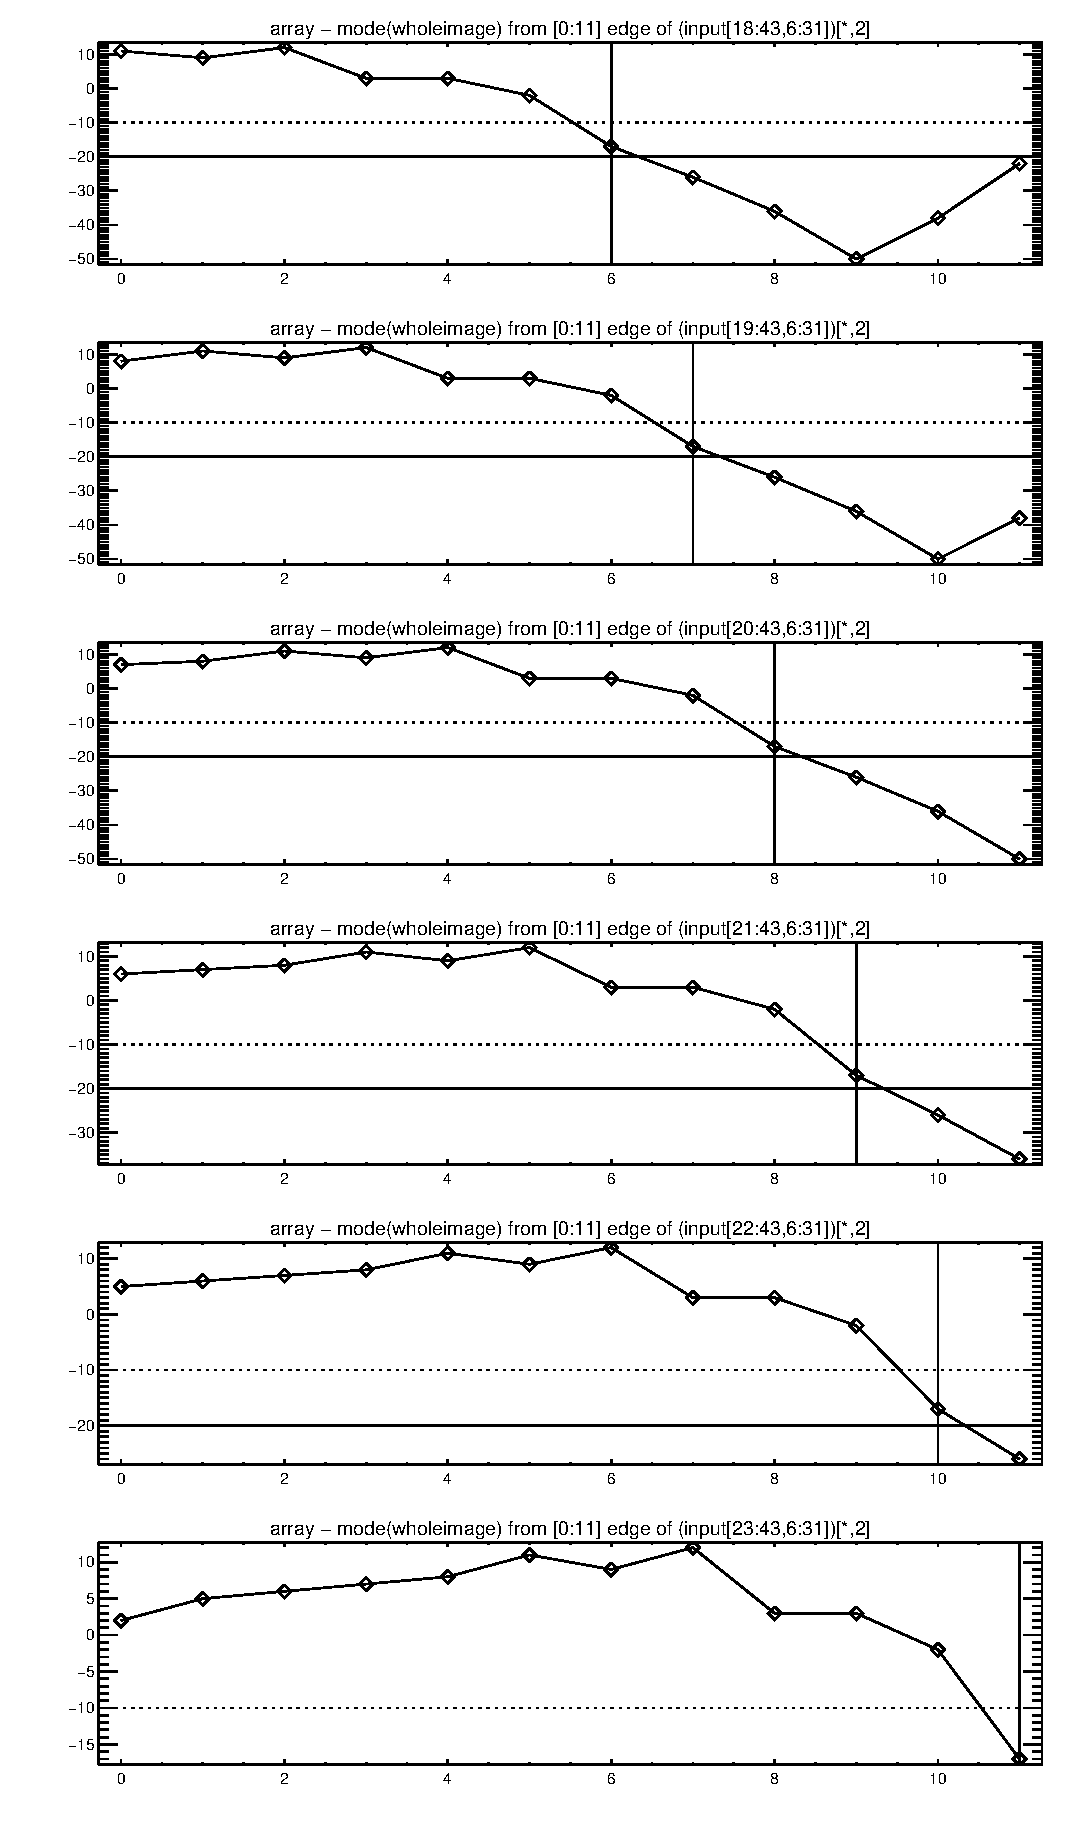
\includegraphics[width=.5\textwidth]{../plots_tables_images/topleft0.eps}%
       }%
       {%
       \caption{Top left, left column}%
       }%
        \ffigbox[\Xhsize]%
       {%
       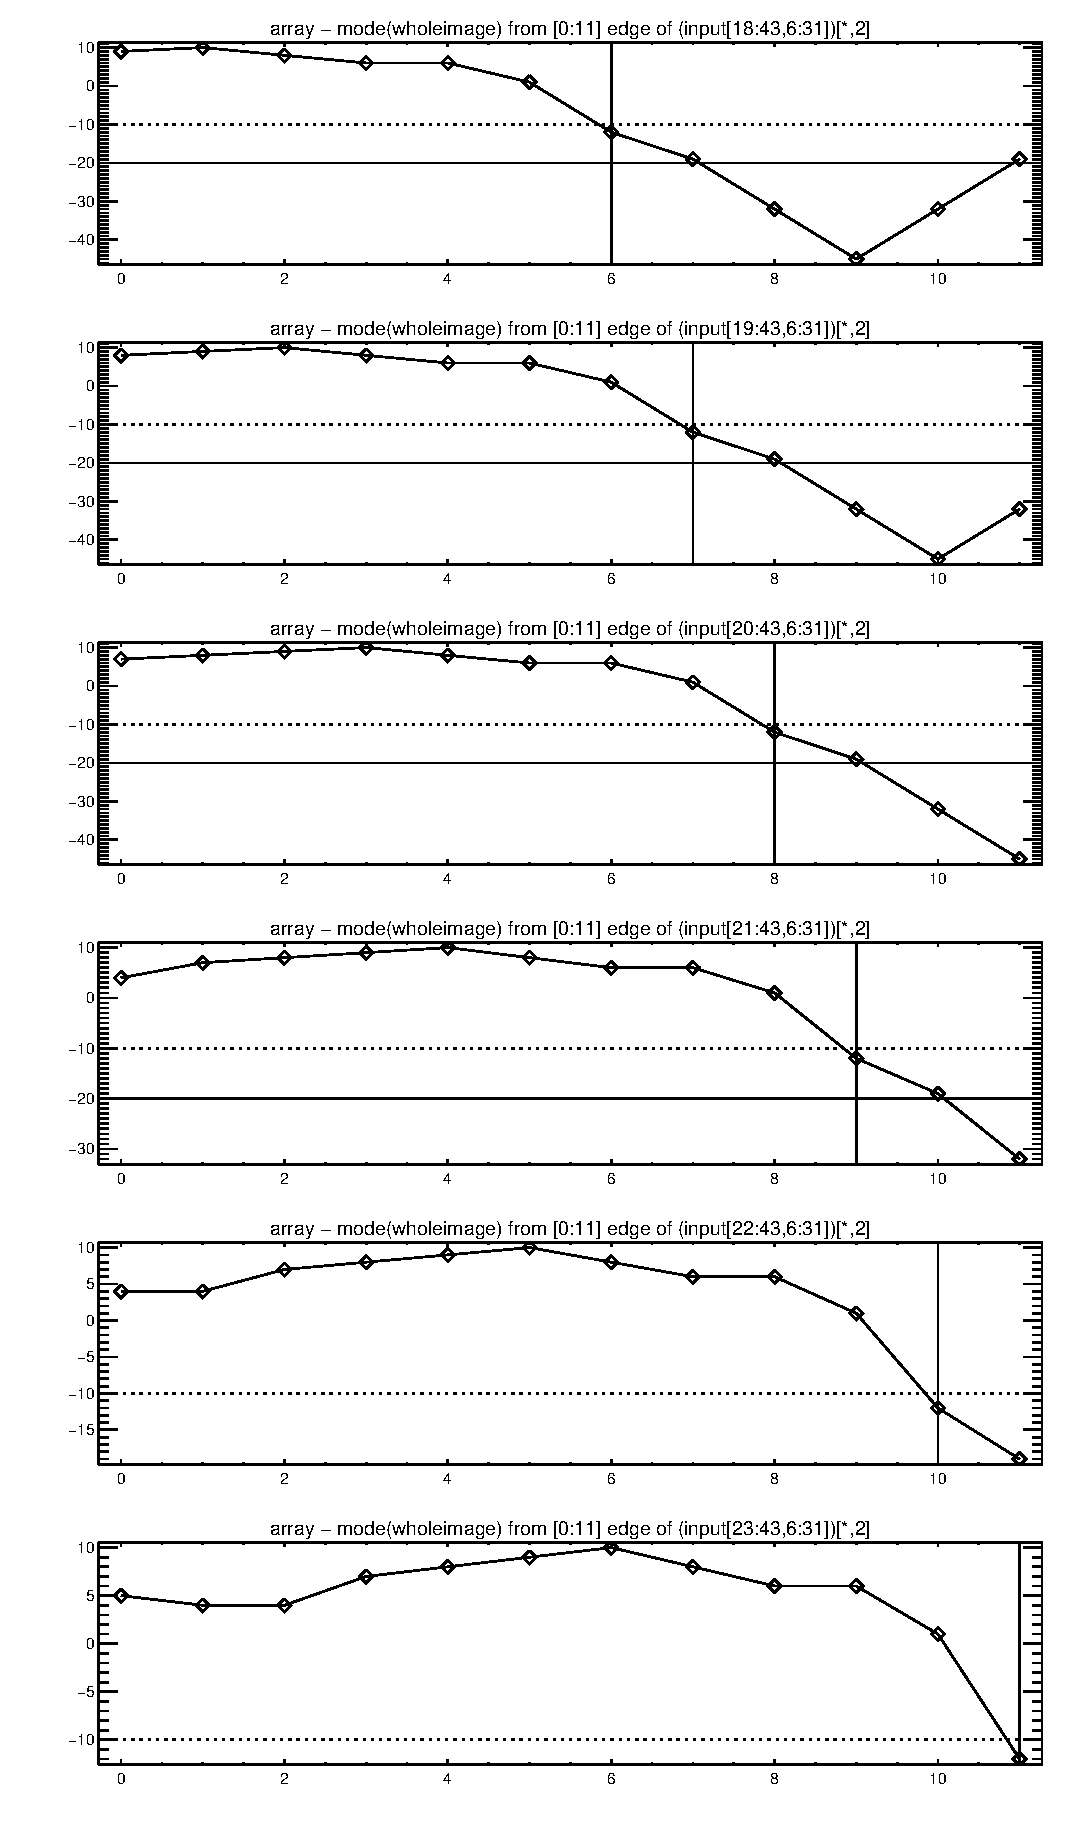
\includegraphics[width=.5\textwidth]{../plots_tables_images/topleft1.eps}%
       }%
       {%
       \caption{Top left, right column}%
       }%
    \end{subfloatrow}}{\caption{}}%
\end{figure}

\begin{figure}[!ht]
    \ffigbox[][\FBheight]{%
    \begin{subfloatrow}[2]%
        \ffigbox[\FBwidth]%
       {%
       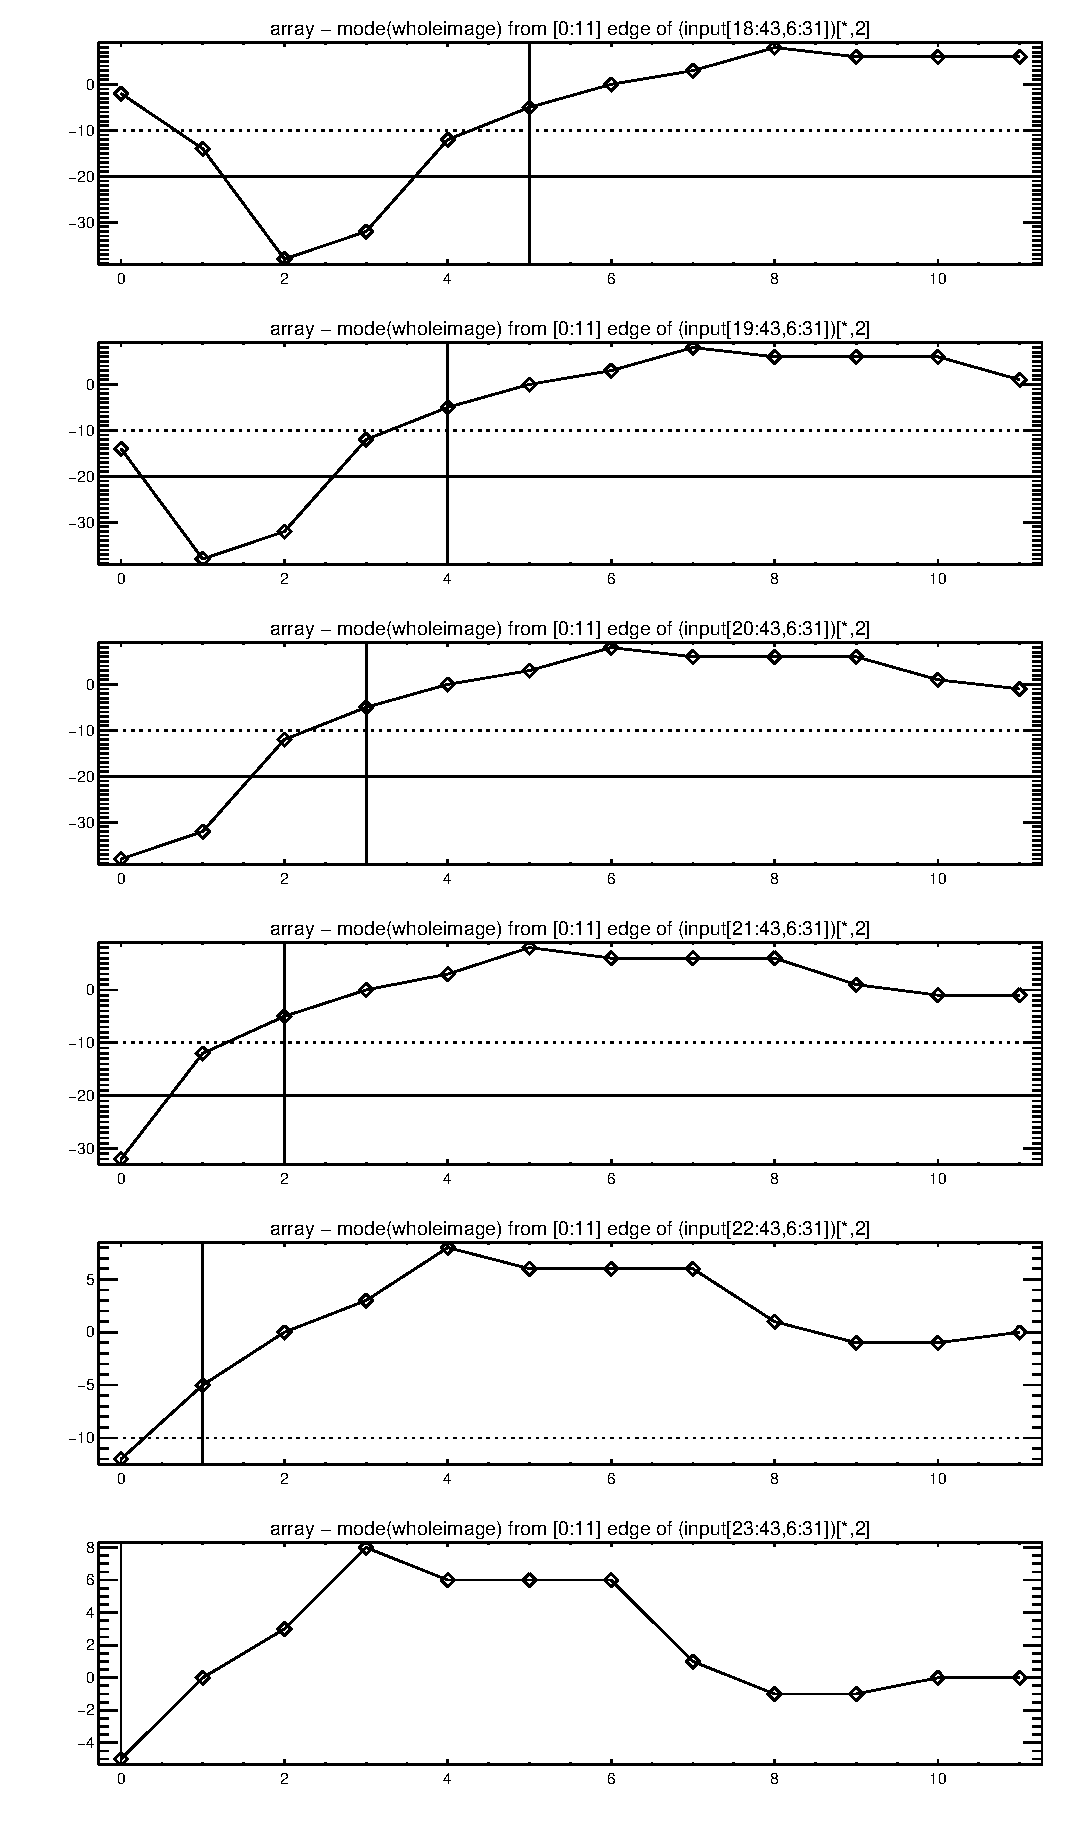
\includegraphics[width=.5\textwidth]{../plots_tables_images/topleft2.eps}%
       }%
       {%
       \caption{Top left, top row}%
       }%
        \ffigbox[\Xhsize]%
       {%
       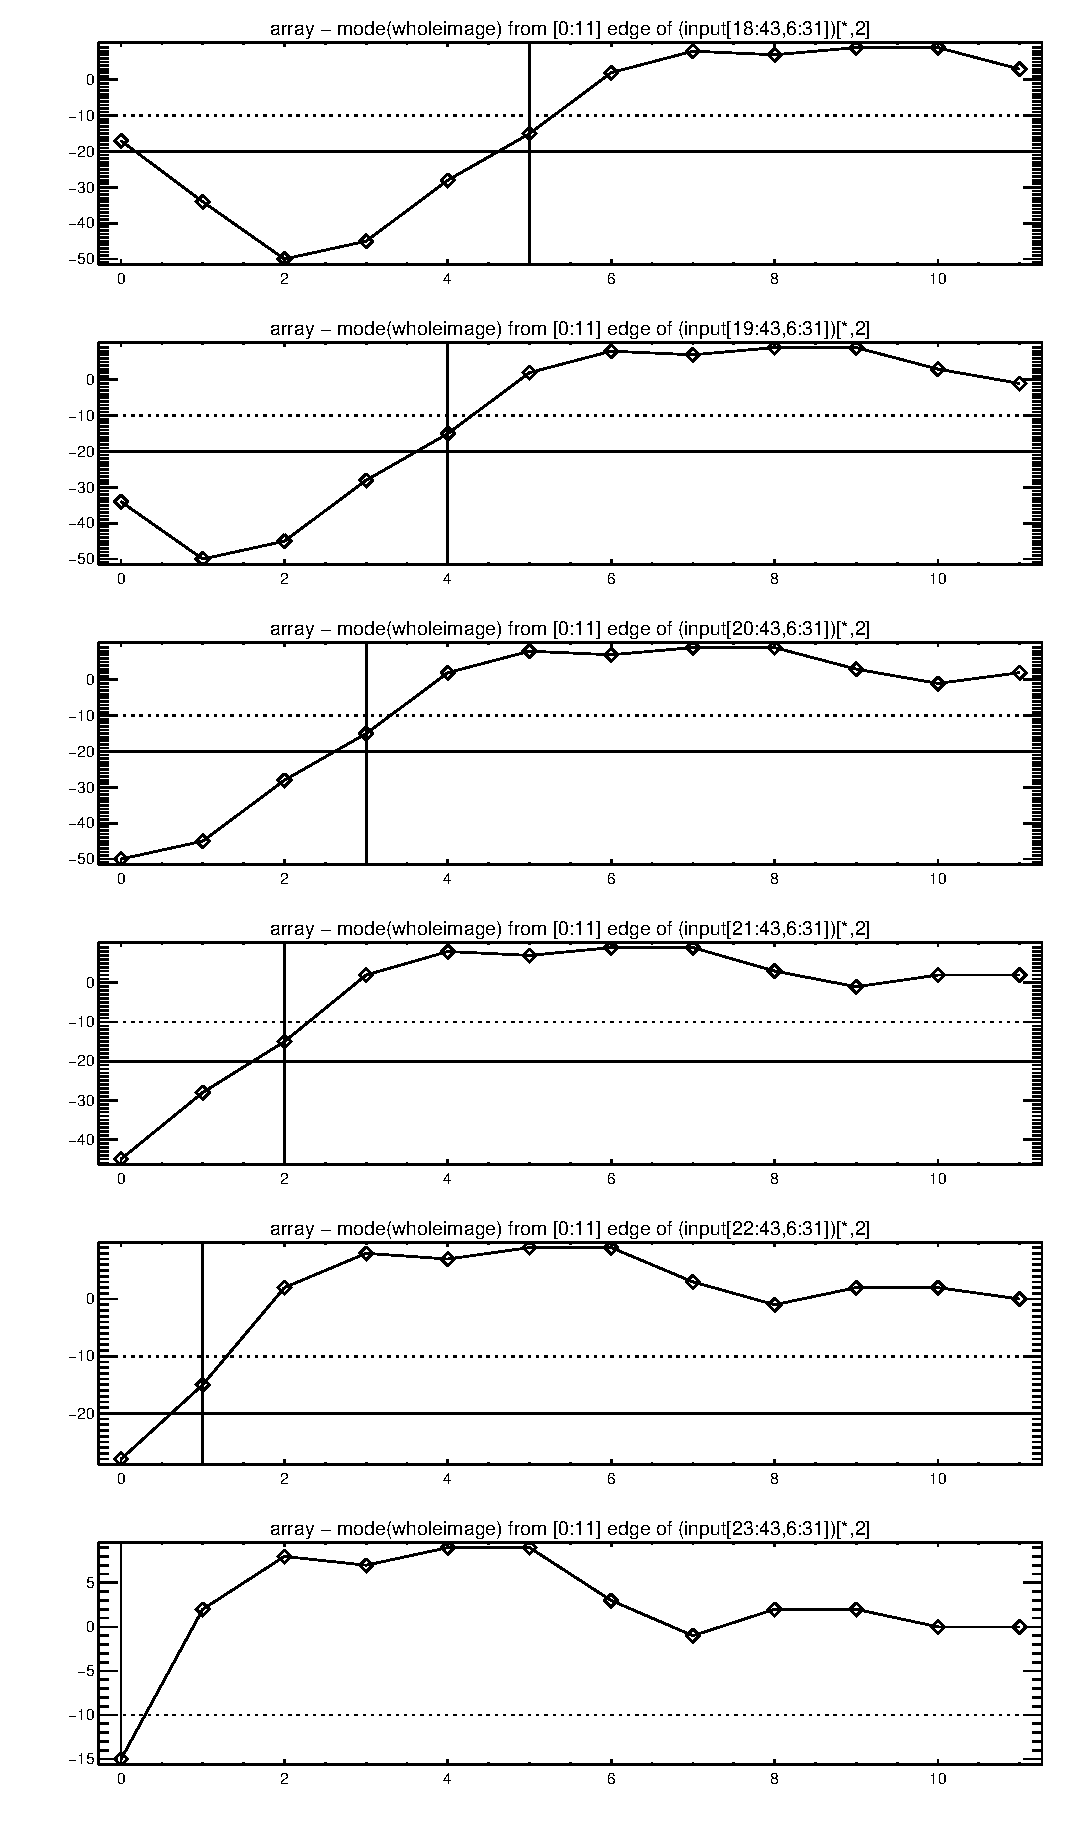
\includegraphics[width=.5\textwidth]{../plots_tables_images/topleft3.eps}%
       }%
       {%
       \caption{Top left, bottom row}%
       }%
    \end{subfloatrow}}{\caption{}}%
\end{figure}

\begin{figure}[!ht]
    \ffigbox[][\FBheight]{%
    \begin{subfloatrow}[2]%
        \ffigbox[\FBwidth]%
       {%
       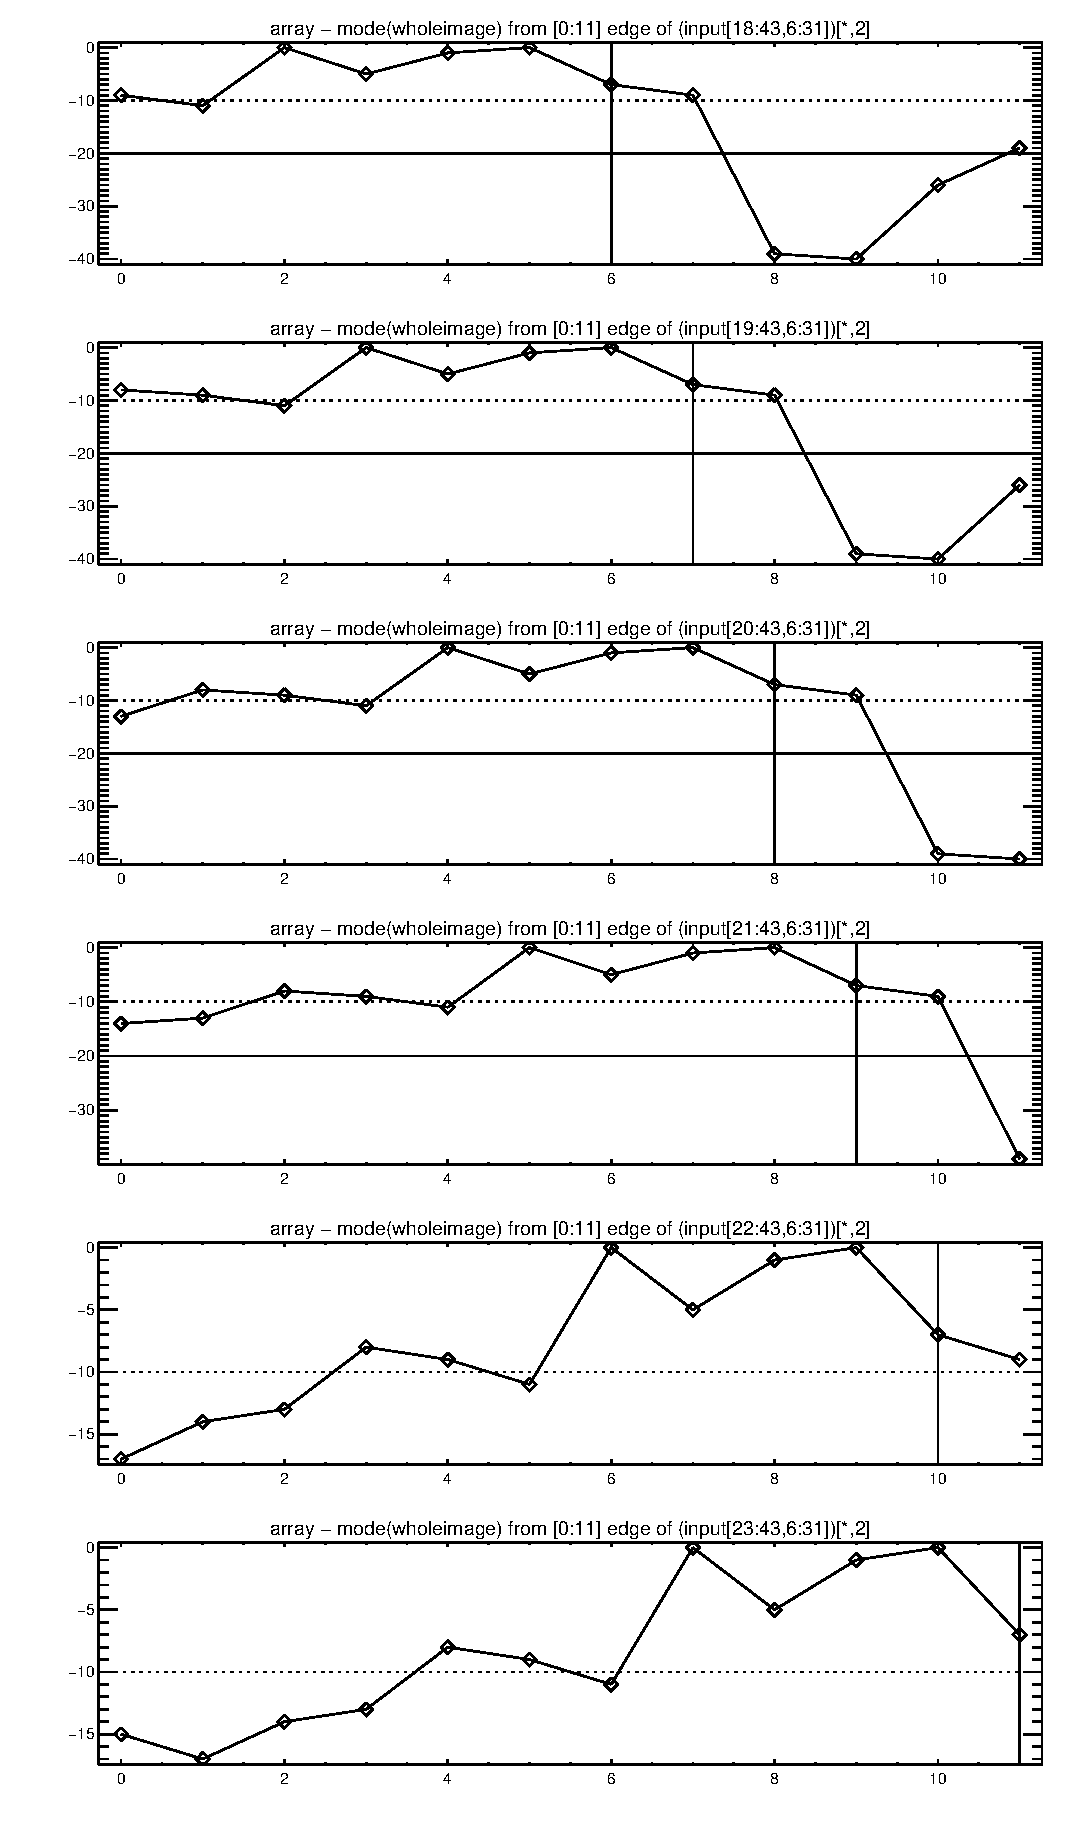
\includegraphics[width=.5\textwidth]{../plots_tables_images/topright0.eps}%
       }%
       {%
       \caption{Top left, right column}%
       }%
        \ffigbox[\Xhsize]%
       {%
       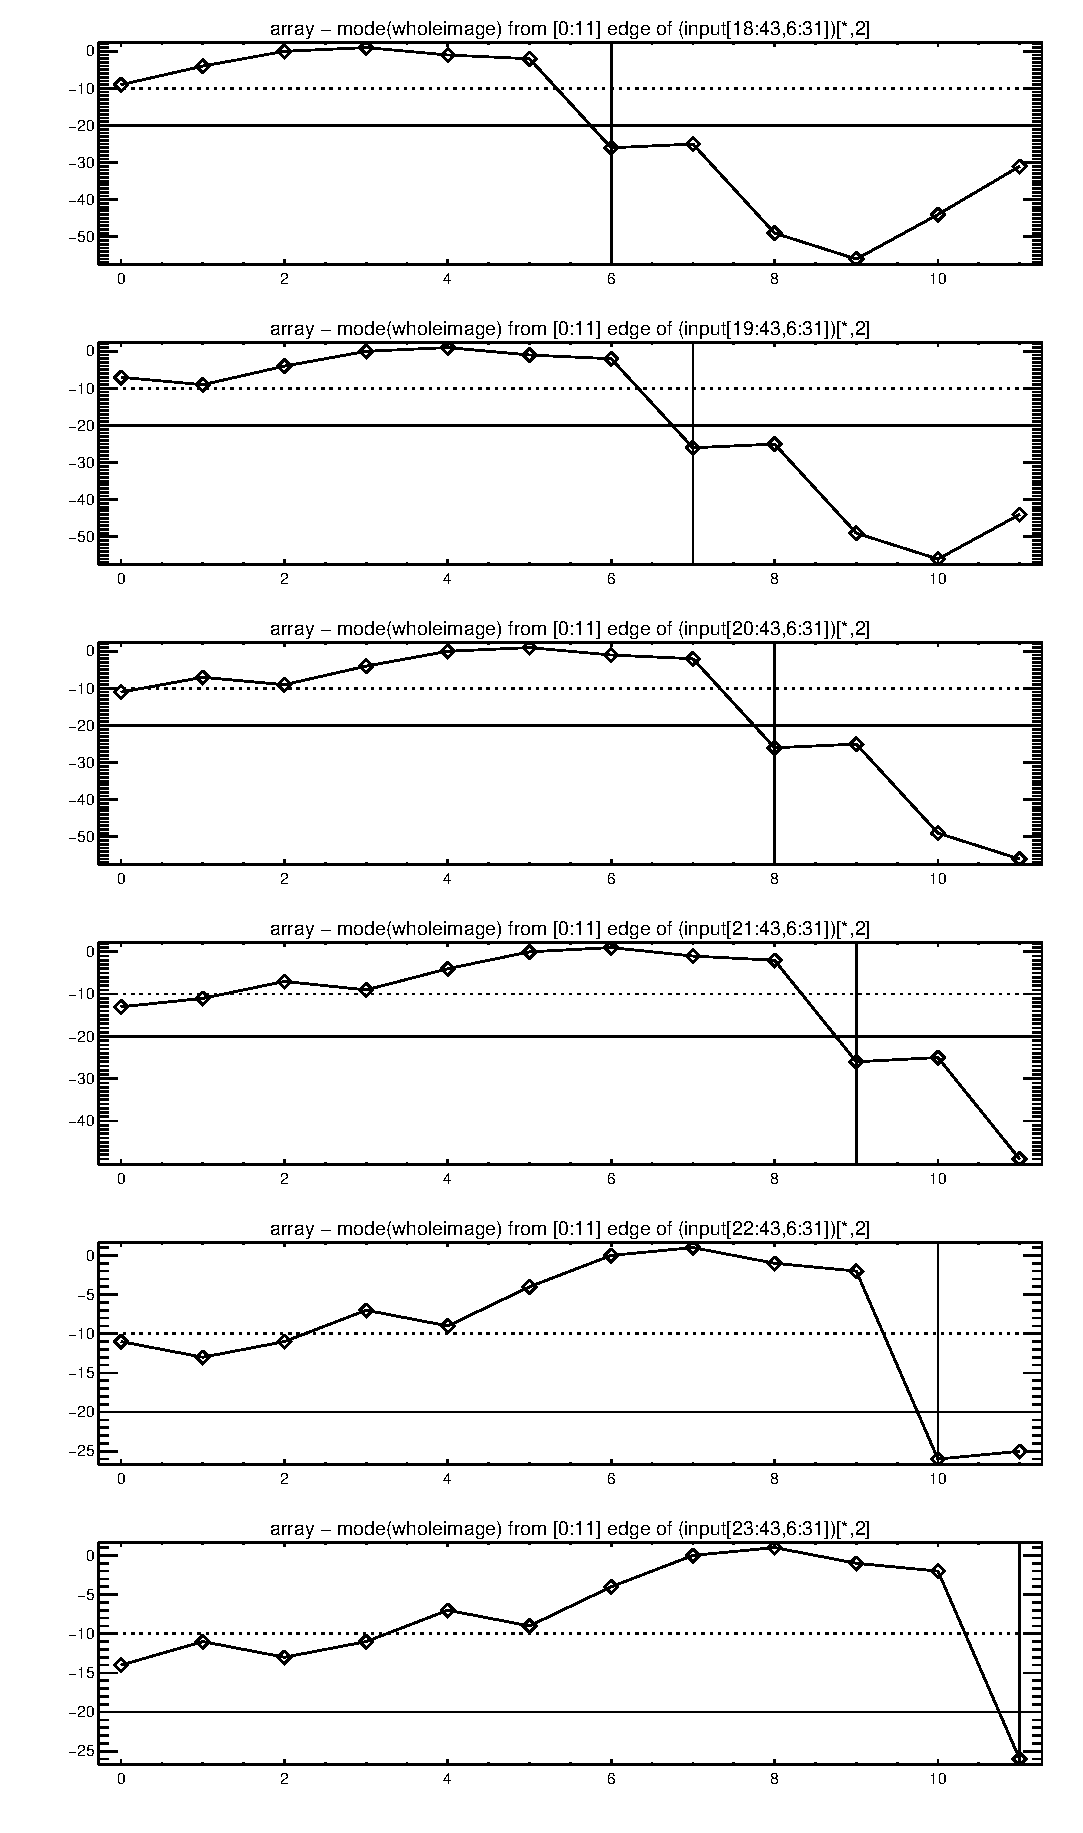
\includegraphics[width=.5\textwidth]{../plots_tables_images/topright1.eps}%
       }%
       {%
       \caption{Top left, left column}%
       }%
    \end{subfloatrow}}{\caption{}}%
\end{figure}

\begin{figure}[!ht]
    \ffigbox[][\FBheight]{%
    \begin{subfloatrow}[2]%
        \ffigbox[\FBwidth]%
       {%
       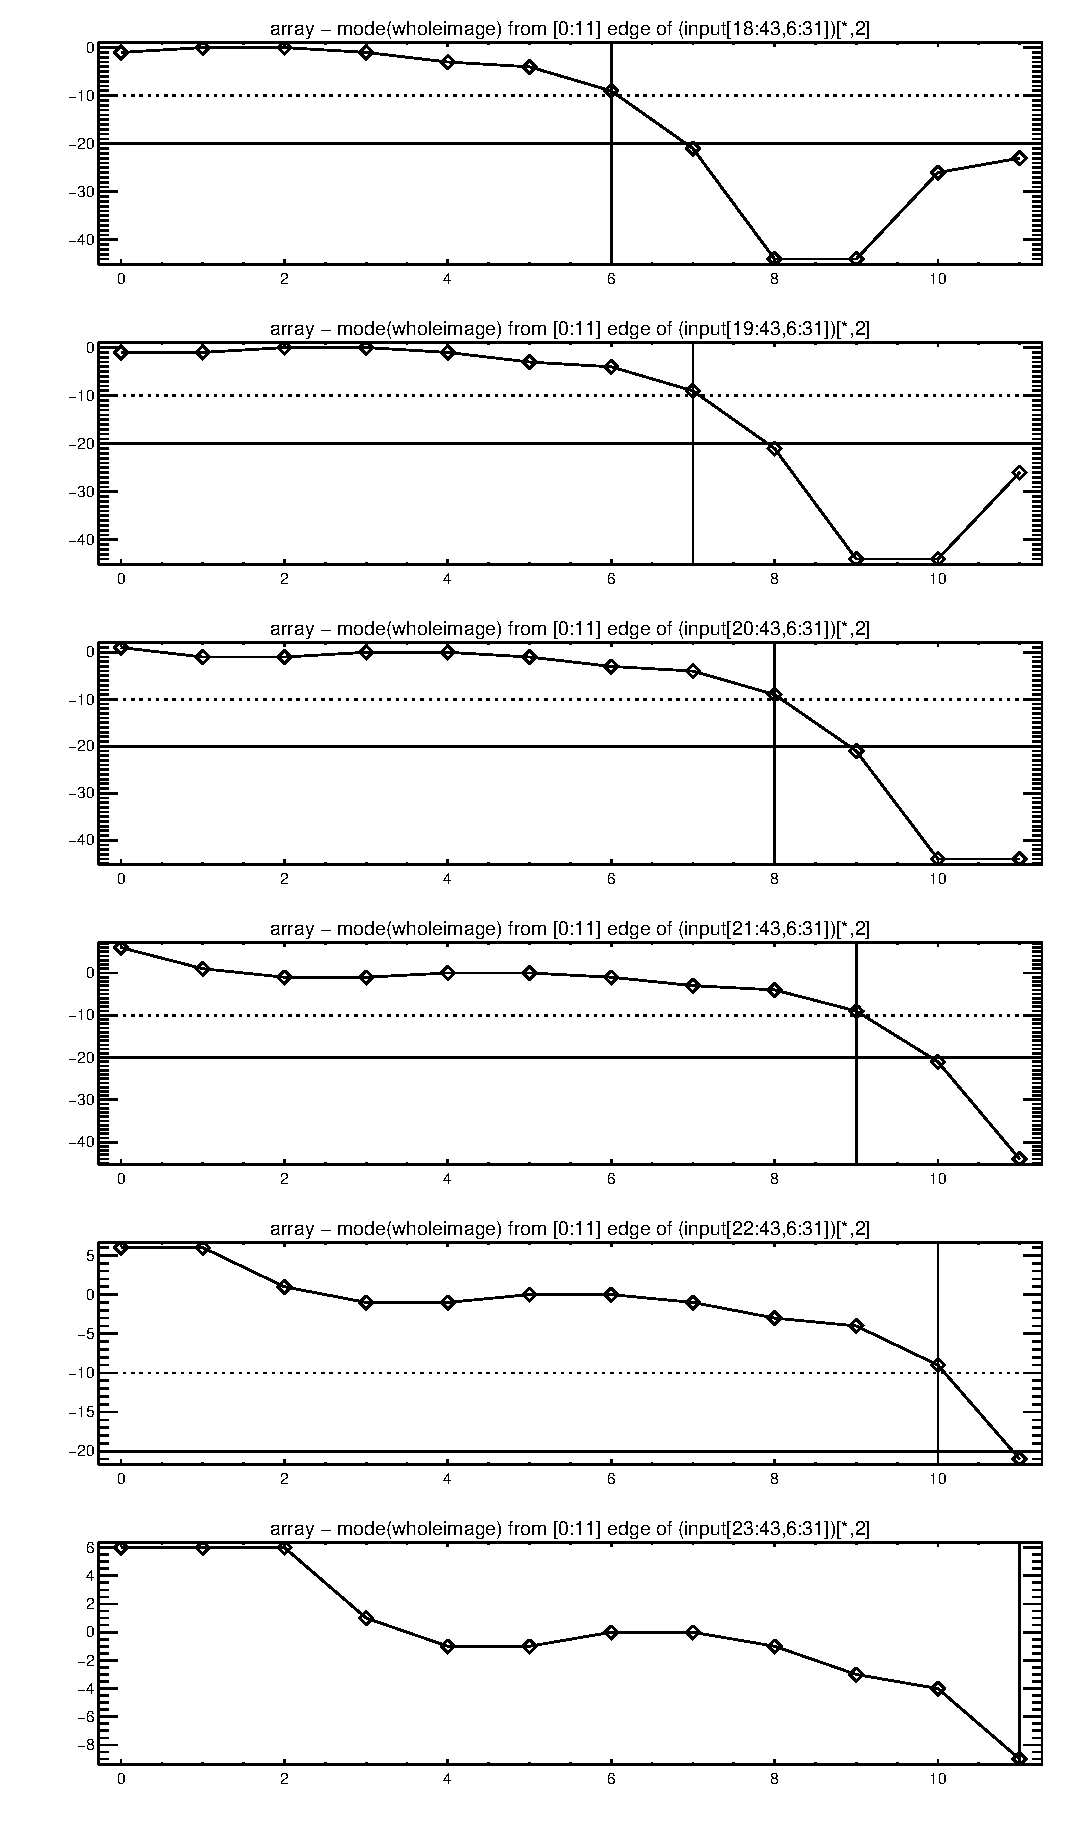
\includegraphics[width=.5\textwidth]{../plots_tables_images/topright2.eps}%
       }%
       {%
       \caption{Top left, top row}%
       }%
        \ffigbox[\Xhsize]%
       {%
       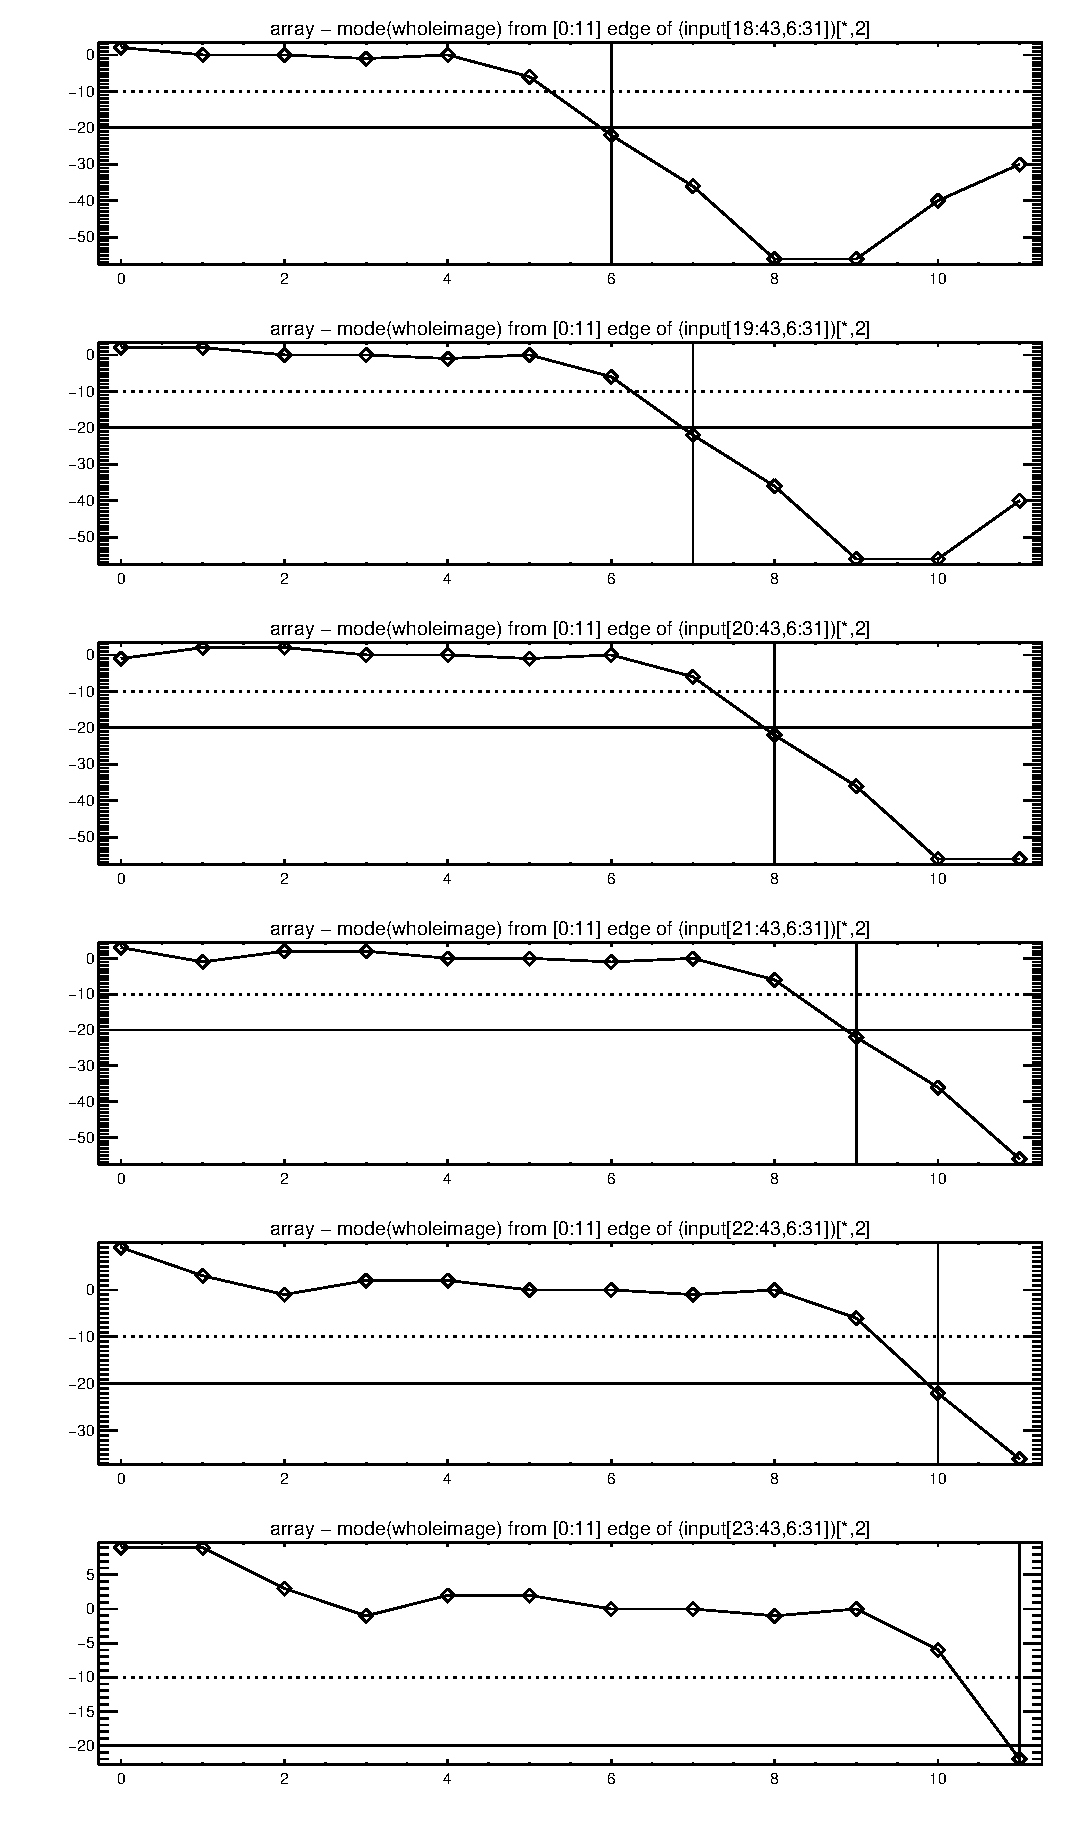
\includegraphics[width=.5\textwidth]{../plots_tables_images/topright3.eps}%
       }%
       {%
       \caption{Top left, bottom row}%
       }%
    \end{subfloatrow}}{\caption{}}%
\end{figure}

% \begin{figure}[!h]
%     \centering 
%     \hspace{-1.0in}
%     \begin{subfigure}[b]{.4\linewidth}
%         \centering
%         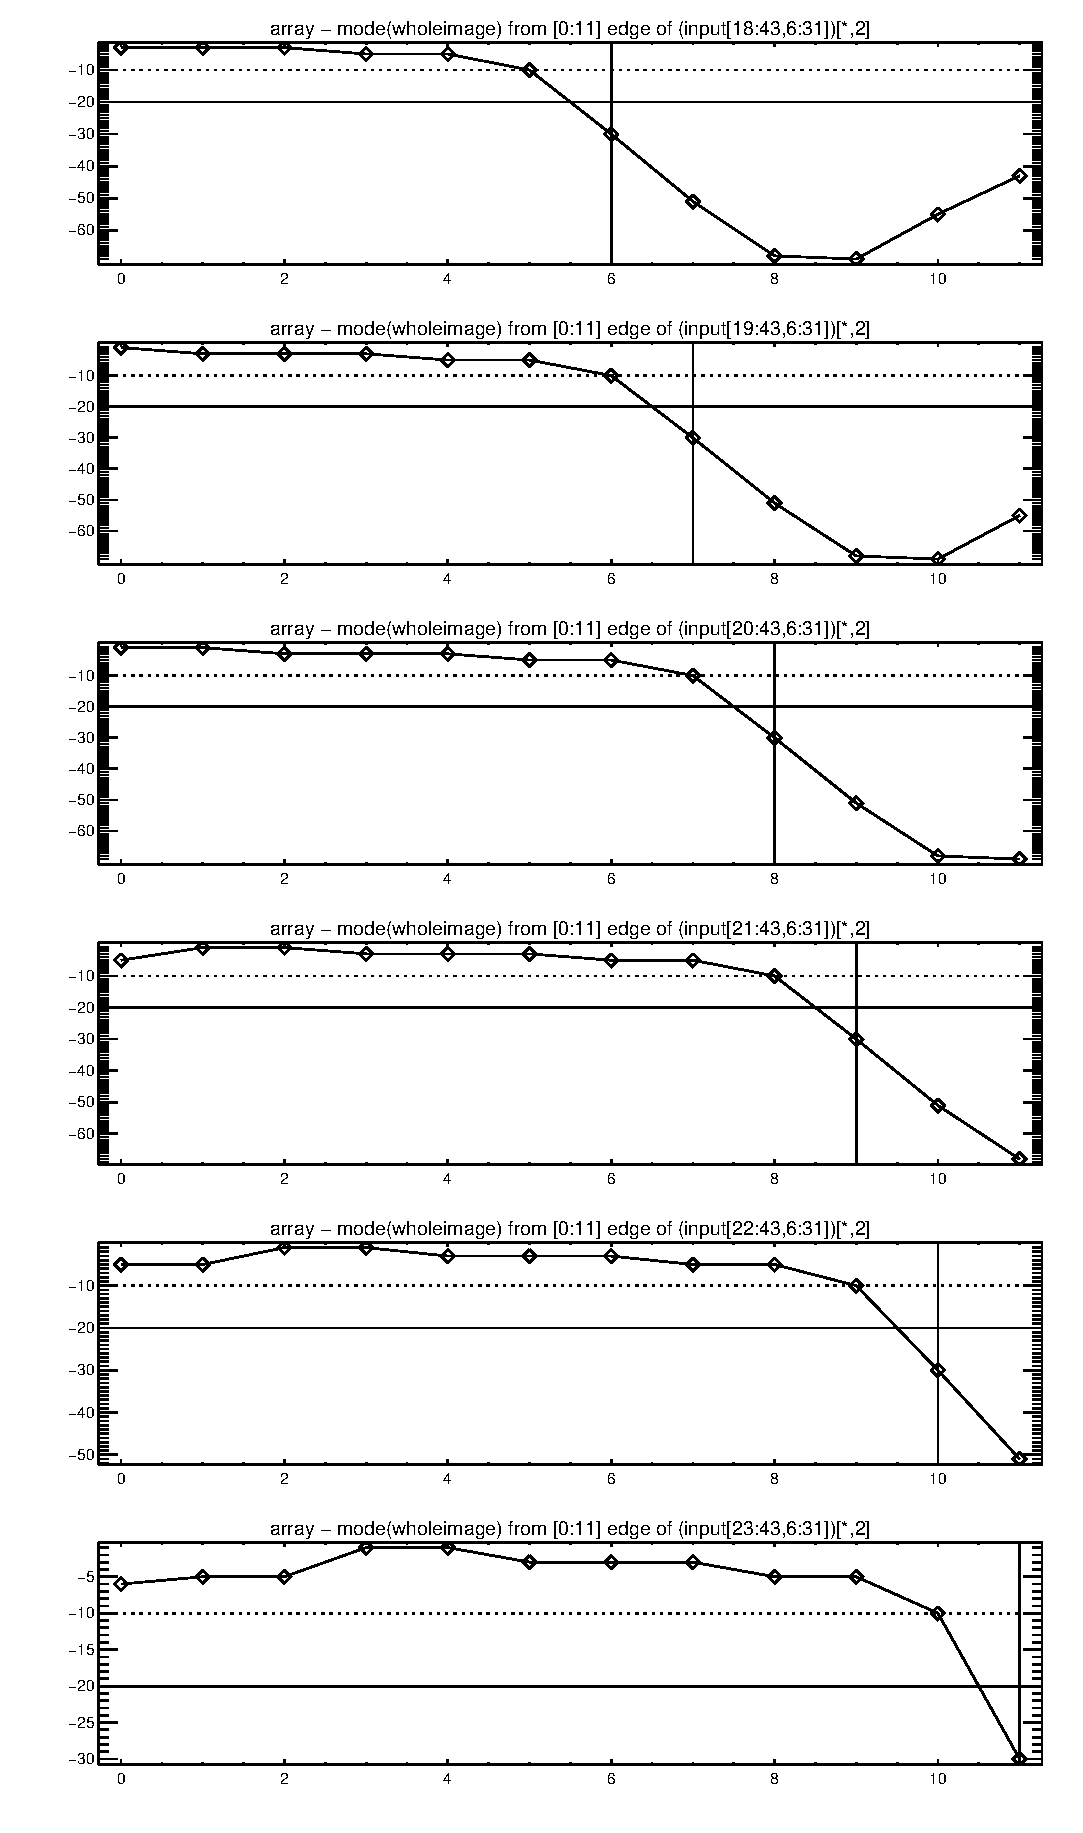
\includegraphics[width=1.4\textwidth]{../plots_tables_images/botright0.eps} 
%         \caption{Bottom right, bottom row}
%     \end{subfigure}
%     \hspace{1.0in}
%     \begin{subfigure}[b]{.4\linewidth}
%         \centering
%         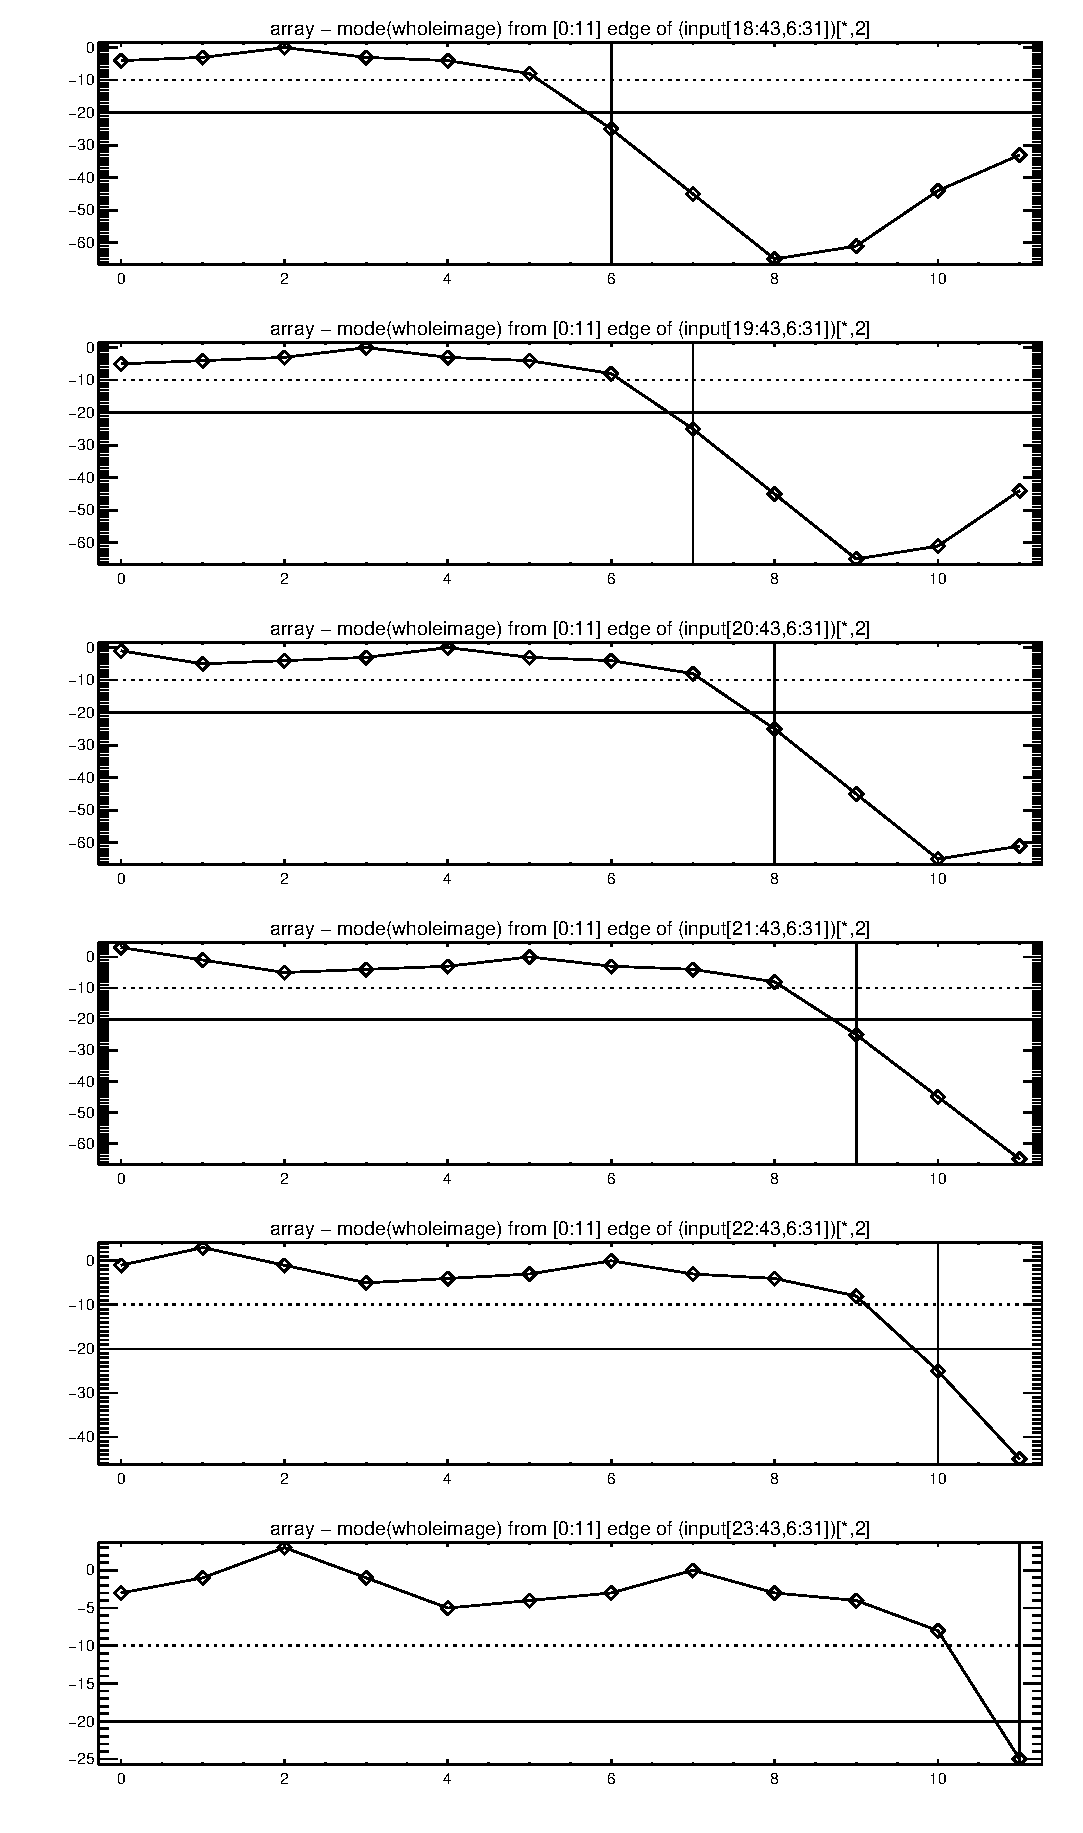
\includegraphics[width=1.4\textwidth]{../plots_tables_images/botright1.eps} 
%         \caption{Bottom right, top row}
%     \end{subfigure}
%     \caption{DUNNO}
% \end{figure}

% \begin{figure}[!h]
%     \centering 
%     \hspace{-1.0in}
%     \begin{subfigure}[b]{.4\linewidth}
%         \centering
%         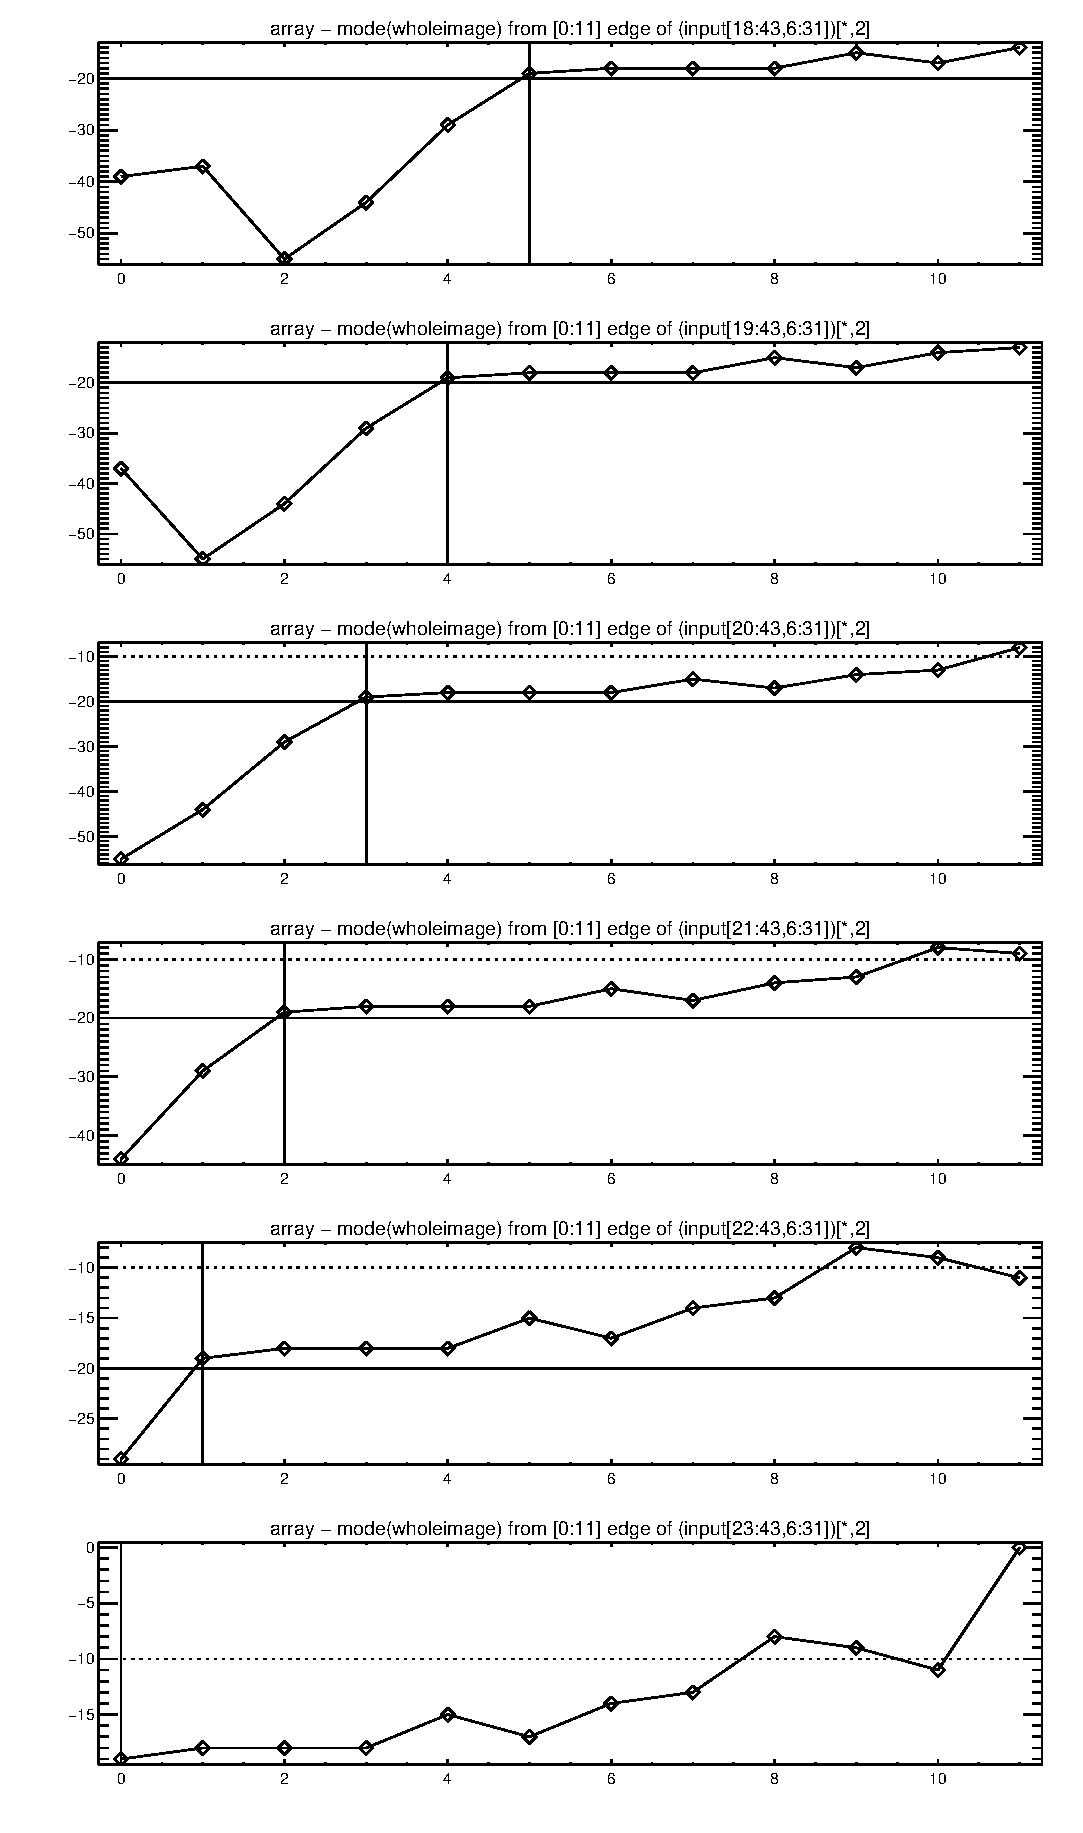
\includegraphics[width=1.4\textwidth]{../plots_tables_images/botright2.eps} 
%         \caption{Bottom right, right column}
%     \end{subfigure}
%     \hspace{1.0in}
%     \begin{subfigure}[b]{.4\linewidth}
%         \centering
%         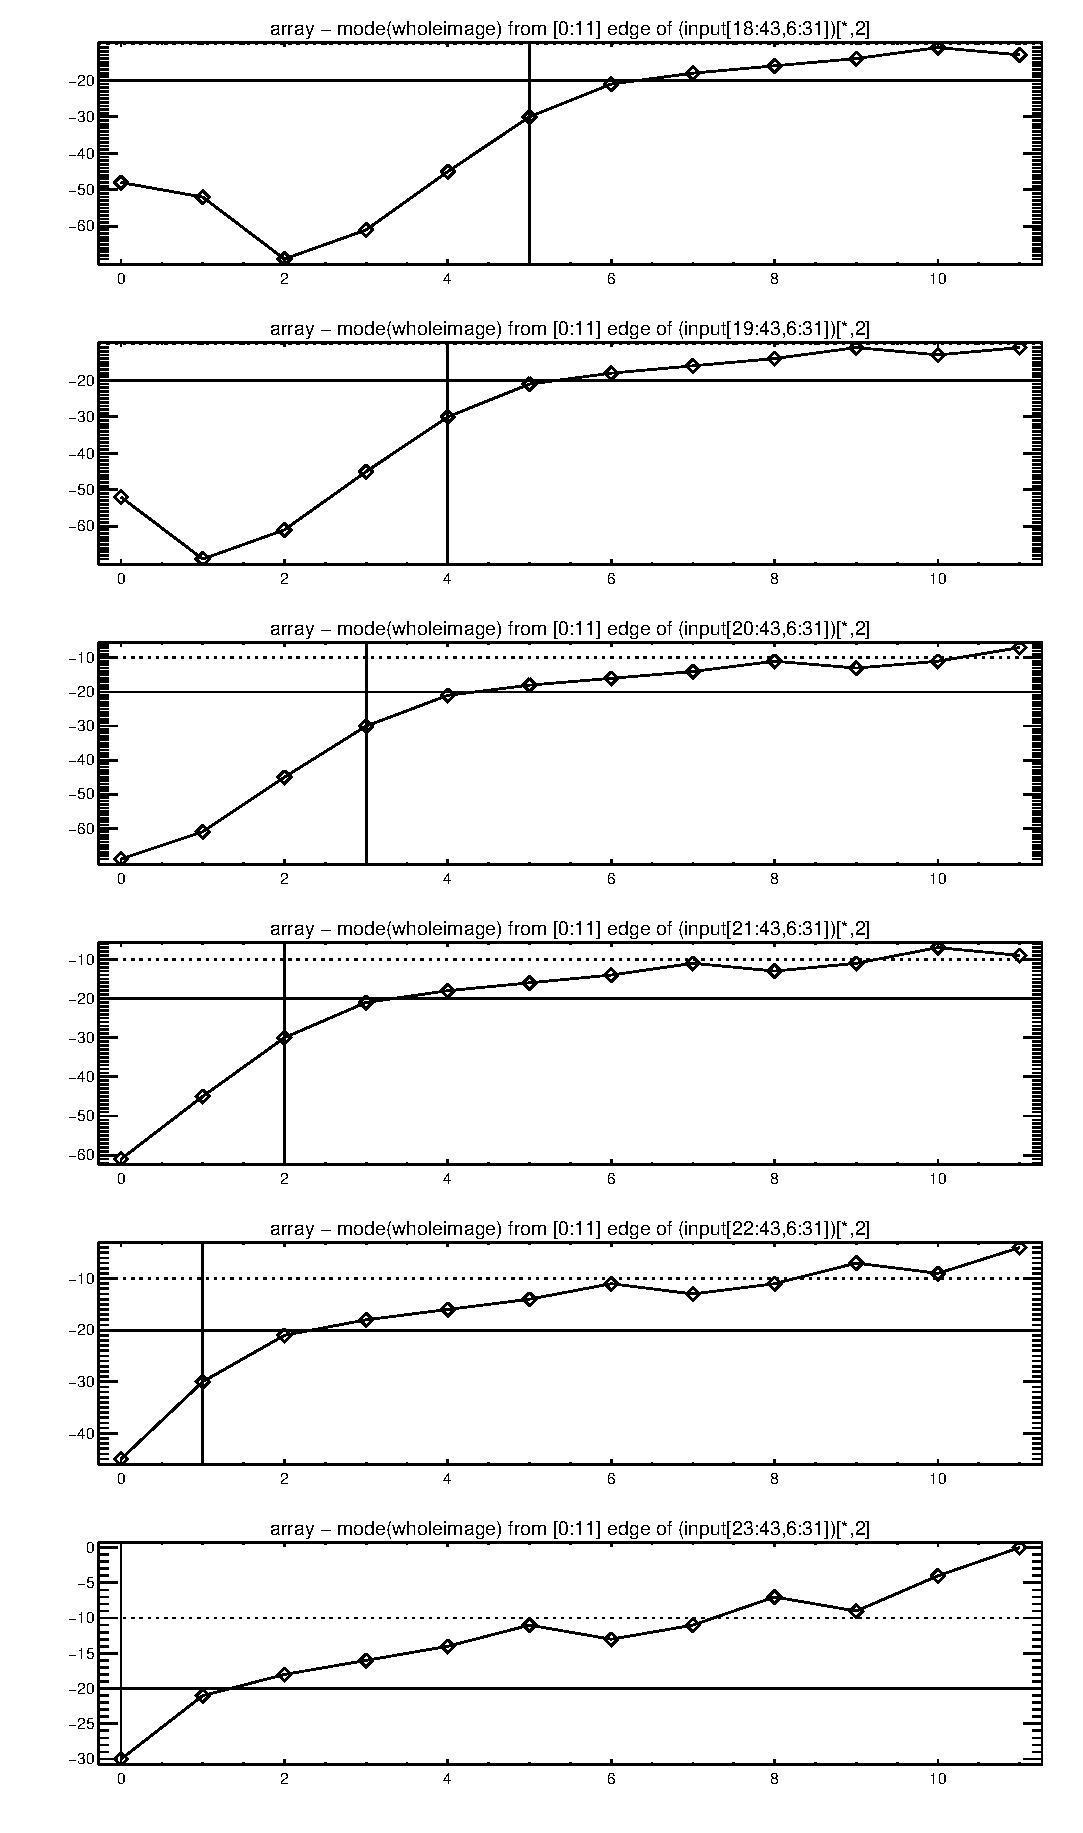
\includegraphics[width=1.4\textwidth]{../plots_tables_images/botright3.eps} 
%         \caption{Bottom right, left column}
%     \end{subfigure}
%     \caption{DUNNO}
% \end{figure}
%
%
%
%
% \begin{figure}[!h]
%     \centering 
%     \hspace{-1.0in}
%     \begin{subfigure}[b]{.4\linewidth}
%         \centering
%         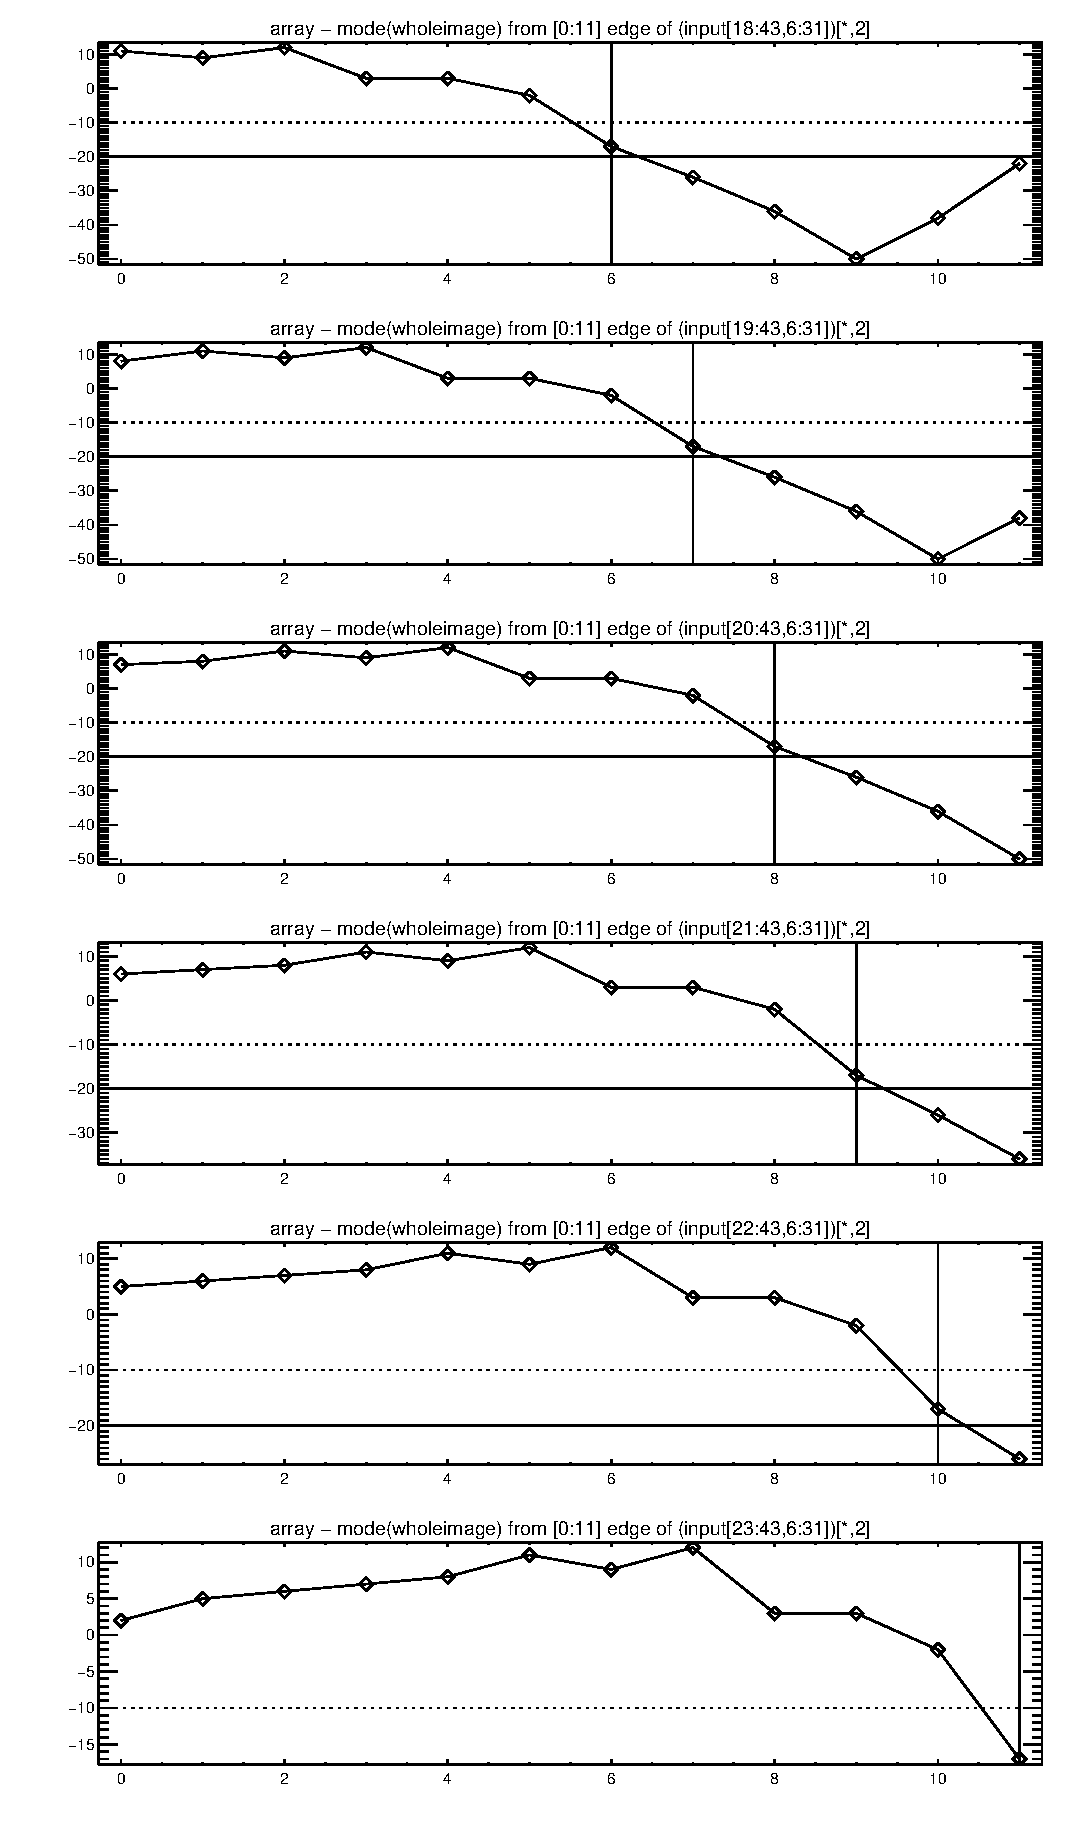
\includegraphics[width=1.4\textwidth]{../plots_tables_images/topleft0.eps} 
%         \caption{Top left, left column}
%     \end{subfigure}
%     \hspace{1.0in}
%     \begin{subfigure}[b]{.4\linewidth}
%         \centering
%         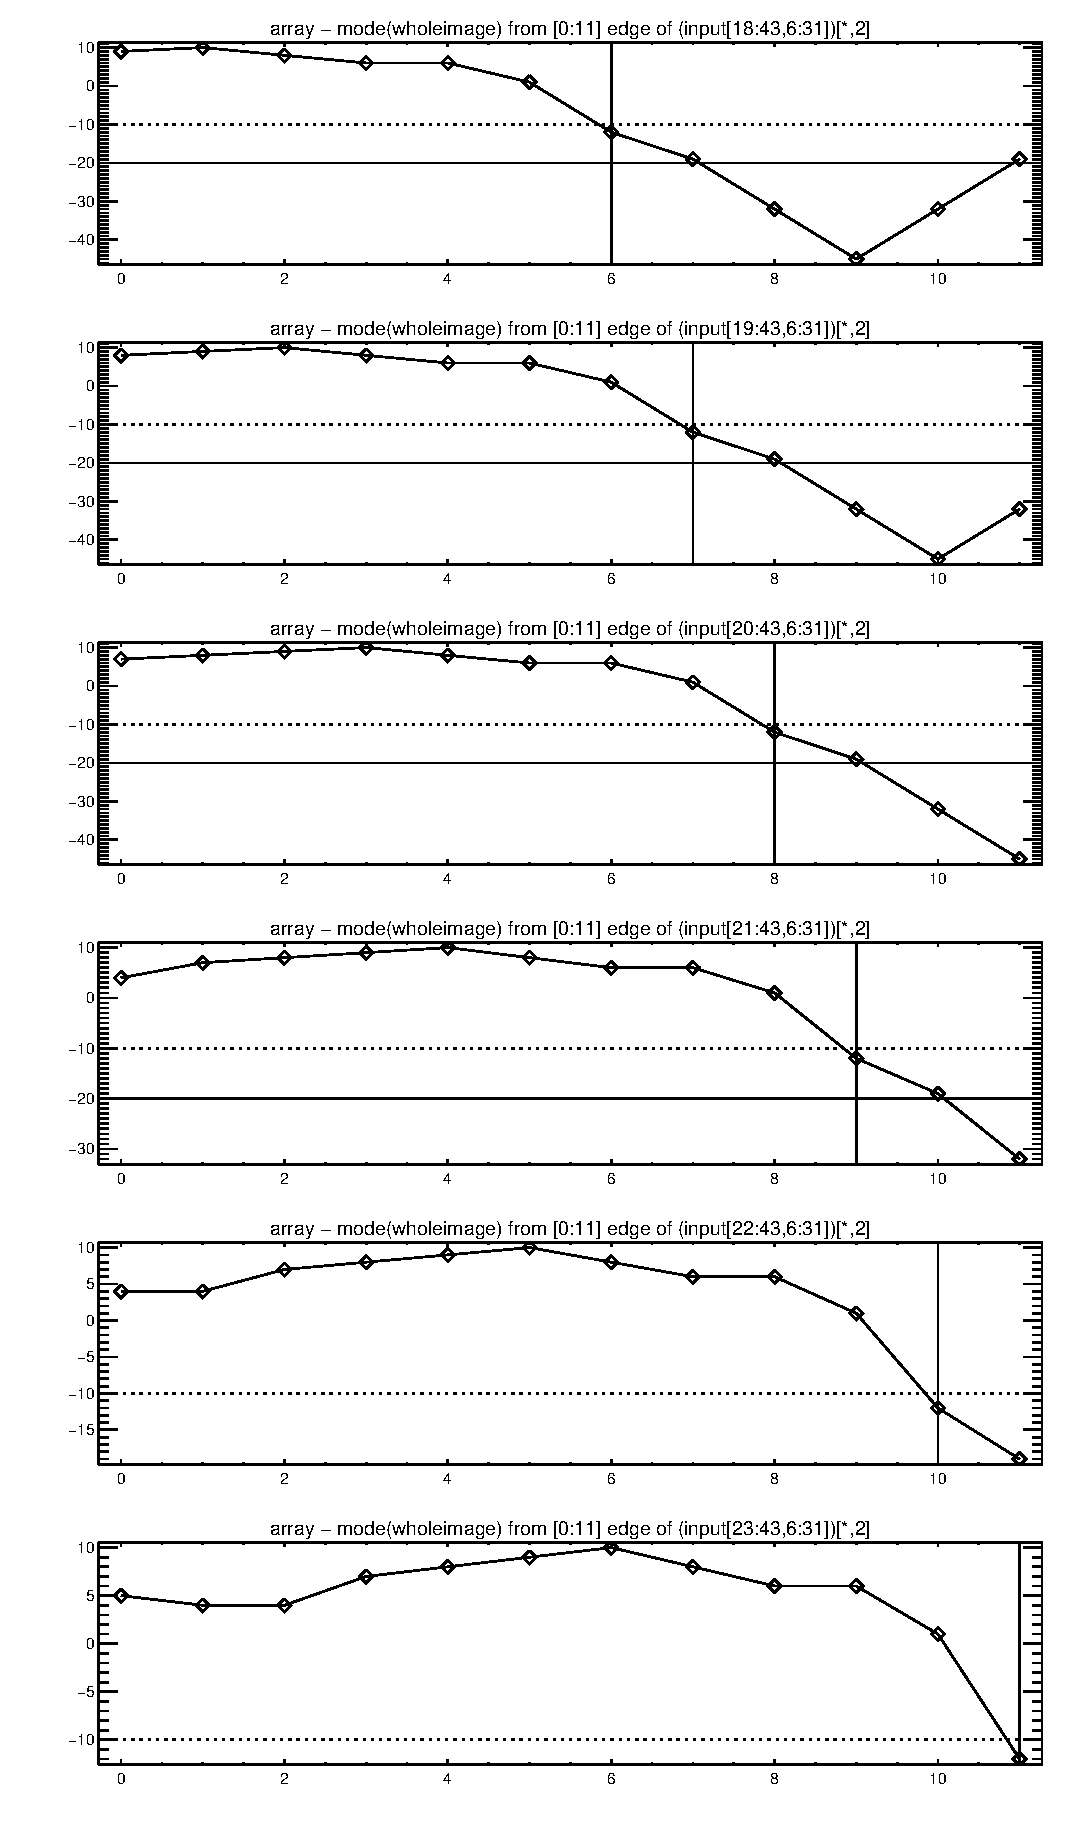
\includegraphics[width=1.4\textwidth]{../plots_tables_images/topleft1.eps} 
%         \caption{Top left, right column}
%     \end{subfigure}
%     \caption{DUNNO}
% \end{figure}

% \begin{figure}[!h]
%     \centering 
%     \hspace{-1.0in}
%     \begin{subfigure}[b]{.4\linewidth}
%         \centering
%         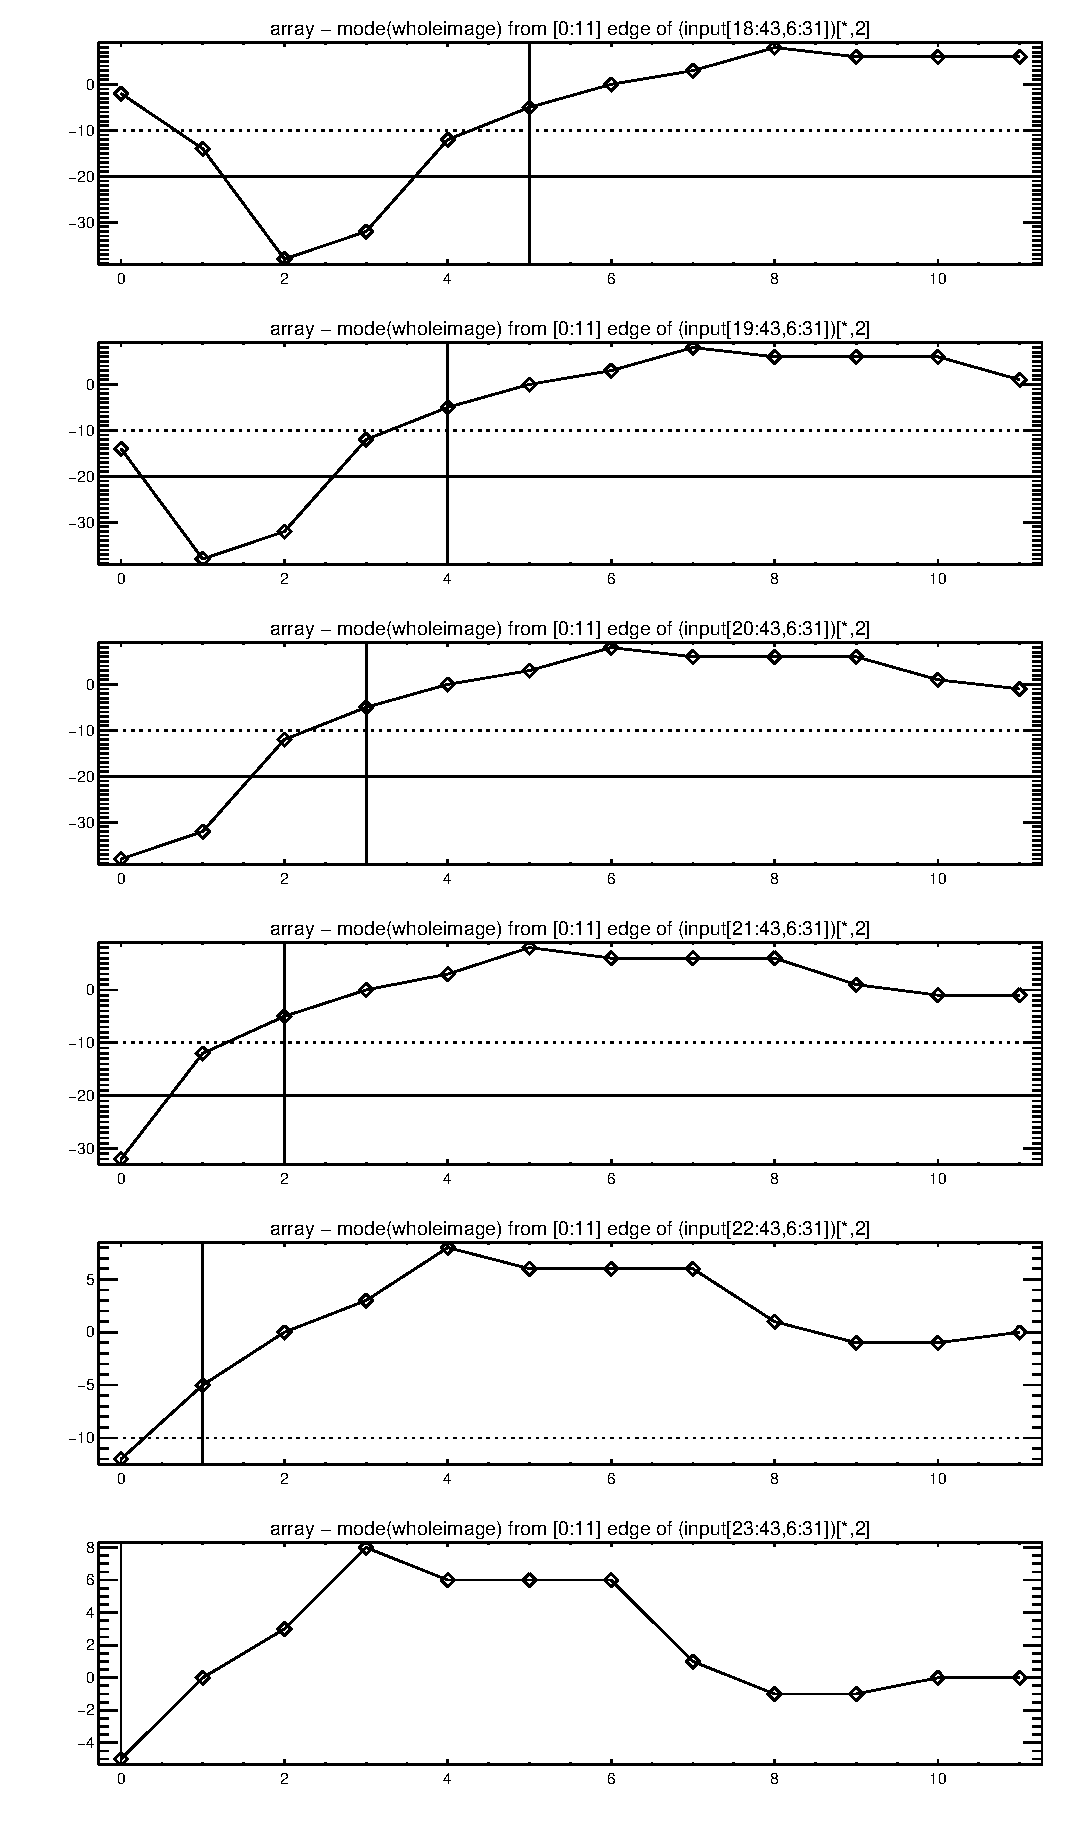
\includegraphics[width=1.4\textwidth]{../plots_tables_images/topleft2.eps} 
%         \caption{Top left, top row}
%     \end{subfigure}
%     \hspace{1.0in}
%     \begin{subfigure}[b]{.4\linewidth}
%         \centering
%         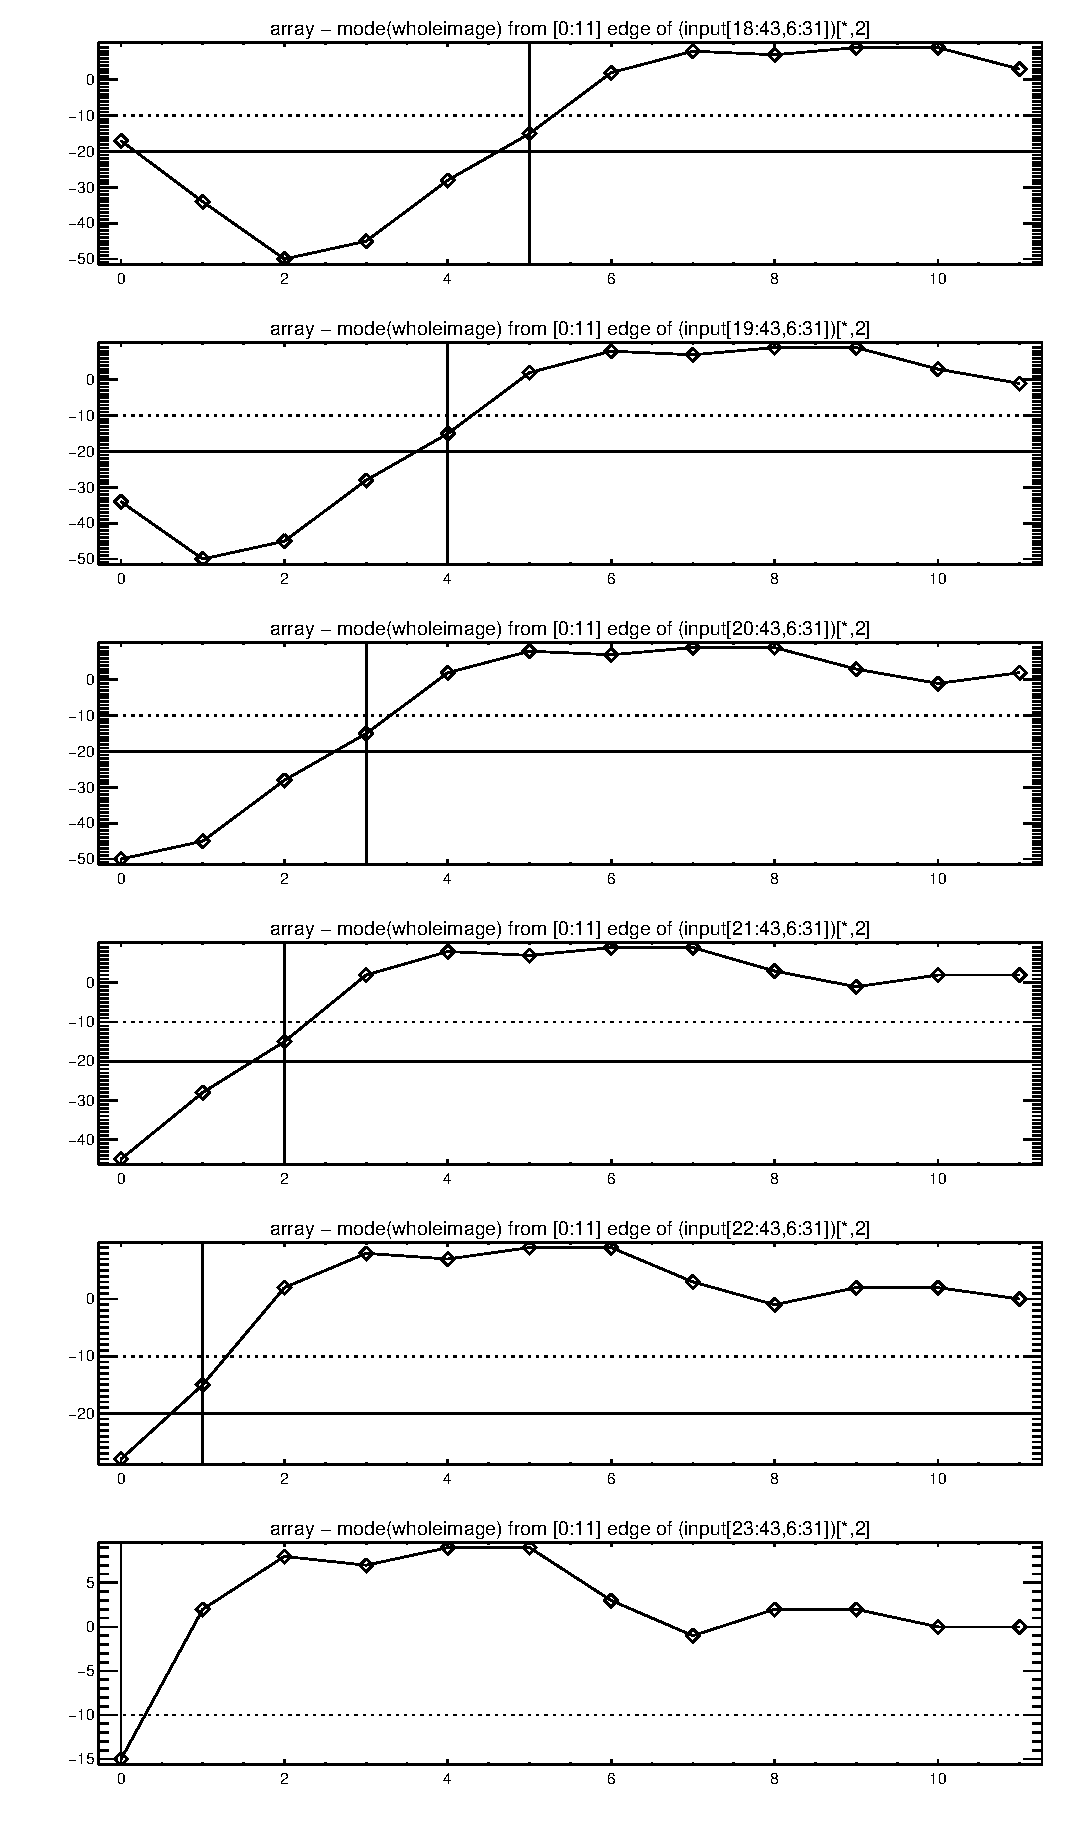
\includegraphics[width=1.4\textwidth]{../plots_tables_images/topleft3.eps} 
%         \caption{Top left, bottom row}
%     \end{subfigure}
%     \caption{DUNNO}
% \end{figure}
% %
% %
% %
% %
% \begin{figure}[!h]
%     \centering 
%     \hspace{-1.0in}
%     \begin{subfigure}[b]{.4\linewidth}
%         \centering
%         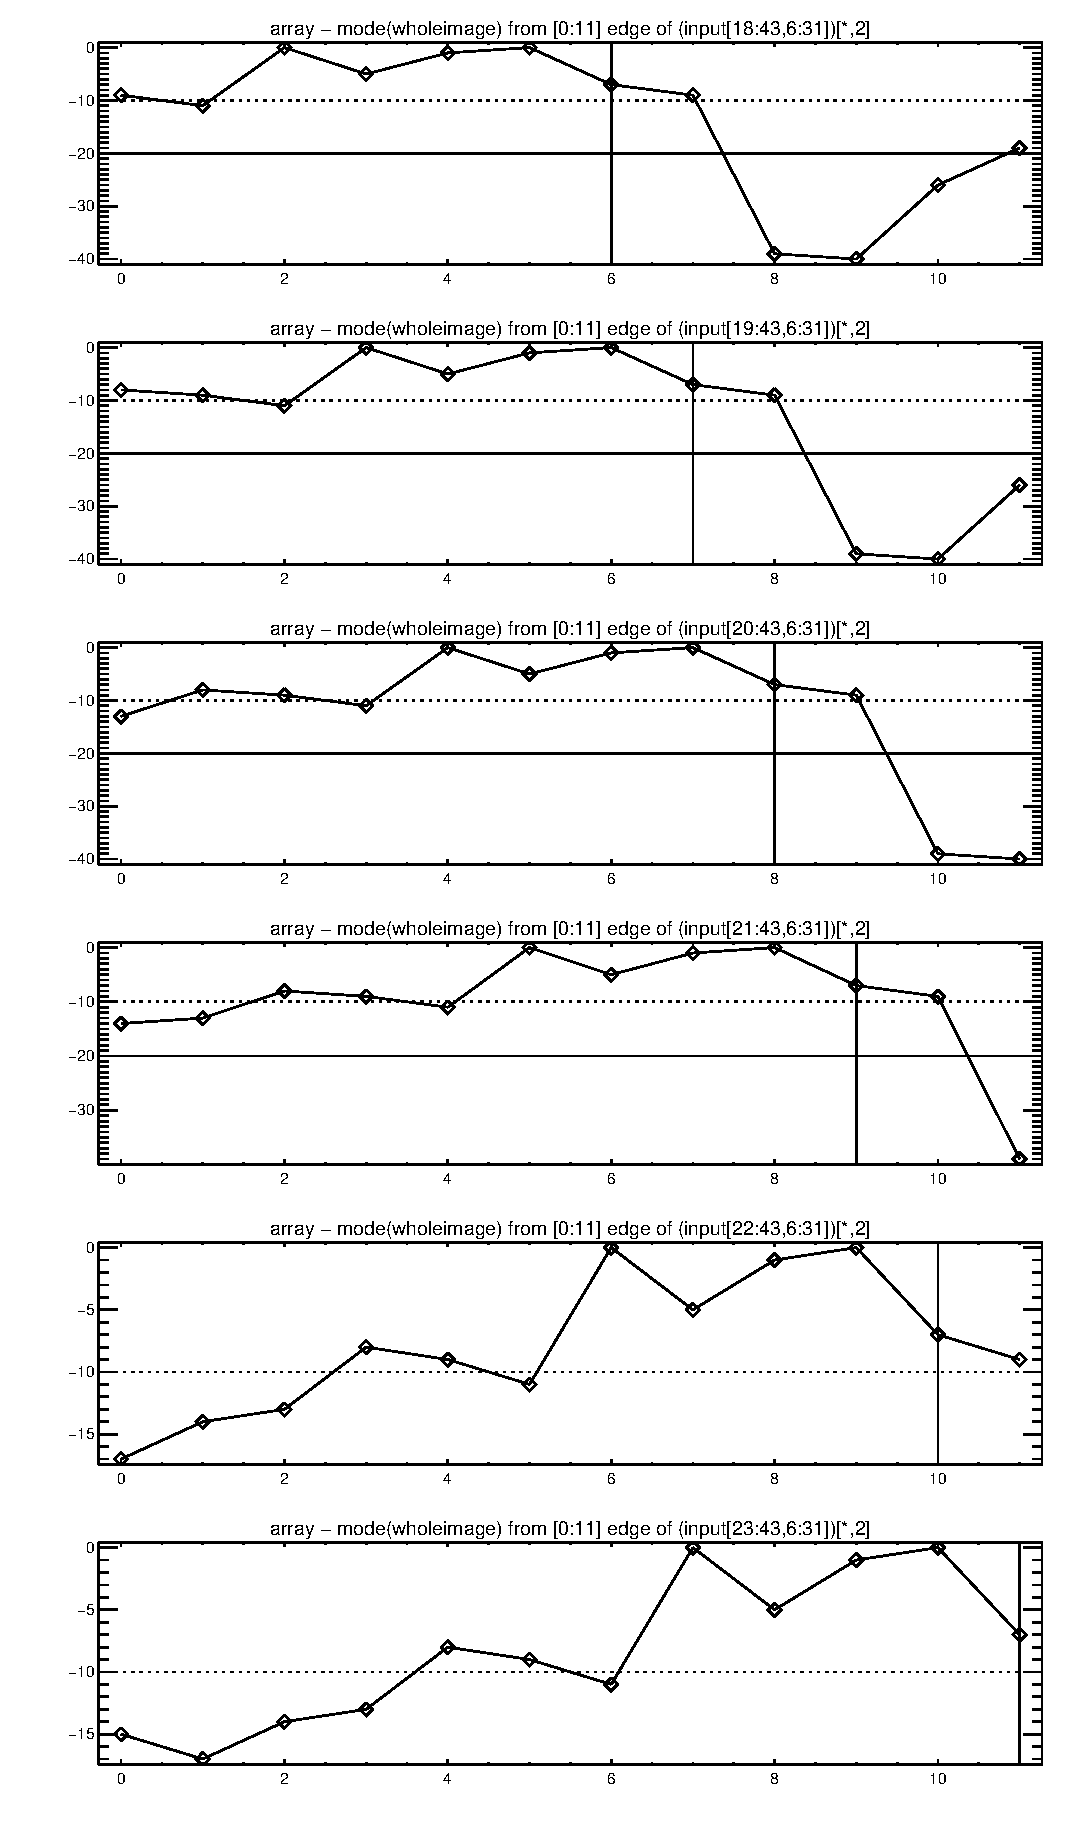
\includegraphics[width=1.4\textwidth]{../plots_tables_images/topright0.eps} 
%         \caption{Top left, right column}
%     \end{subfigure}
%     \hspace{1.0in}
%     \begin{subfigure}[b]{.4\linewidth}
%         \centering
%         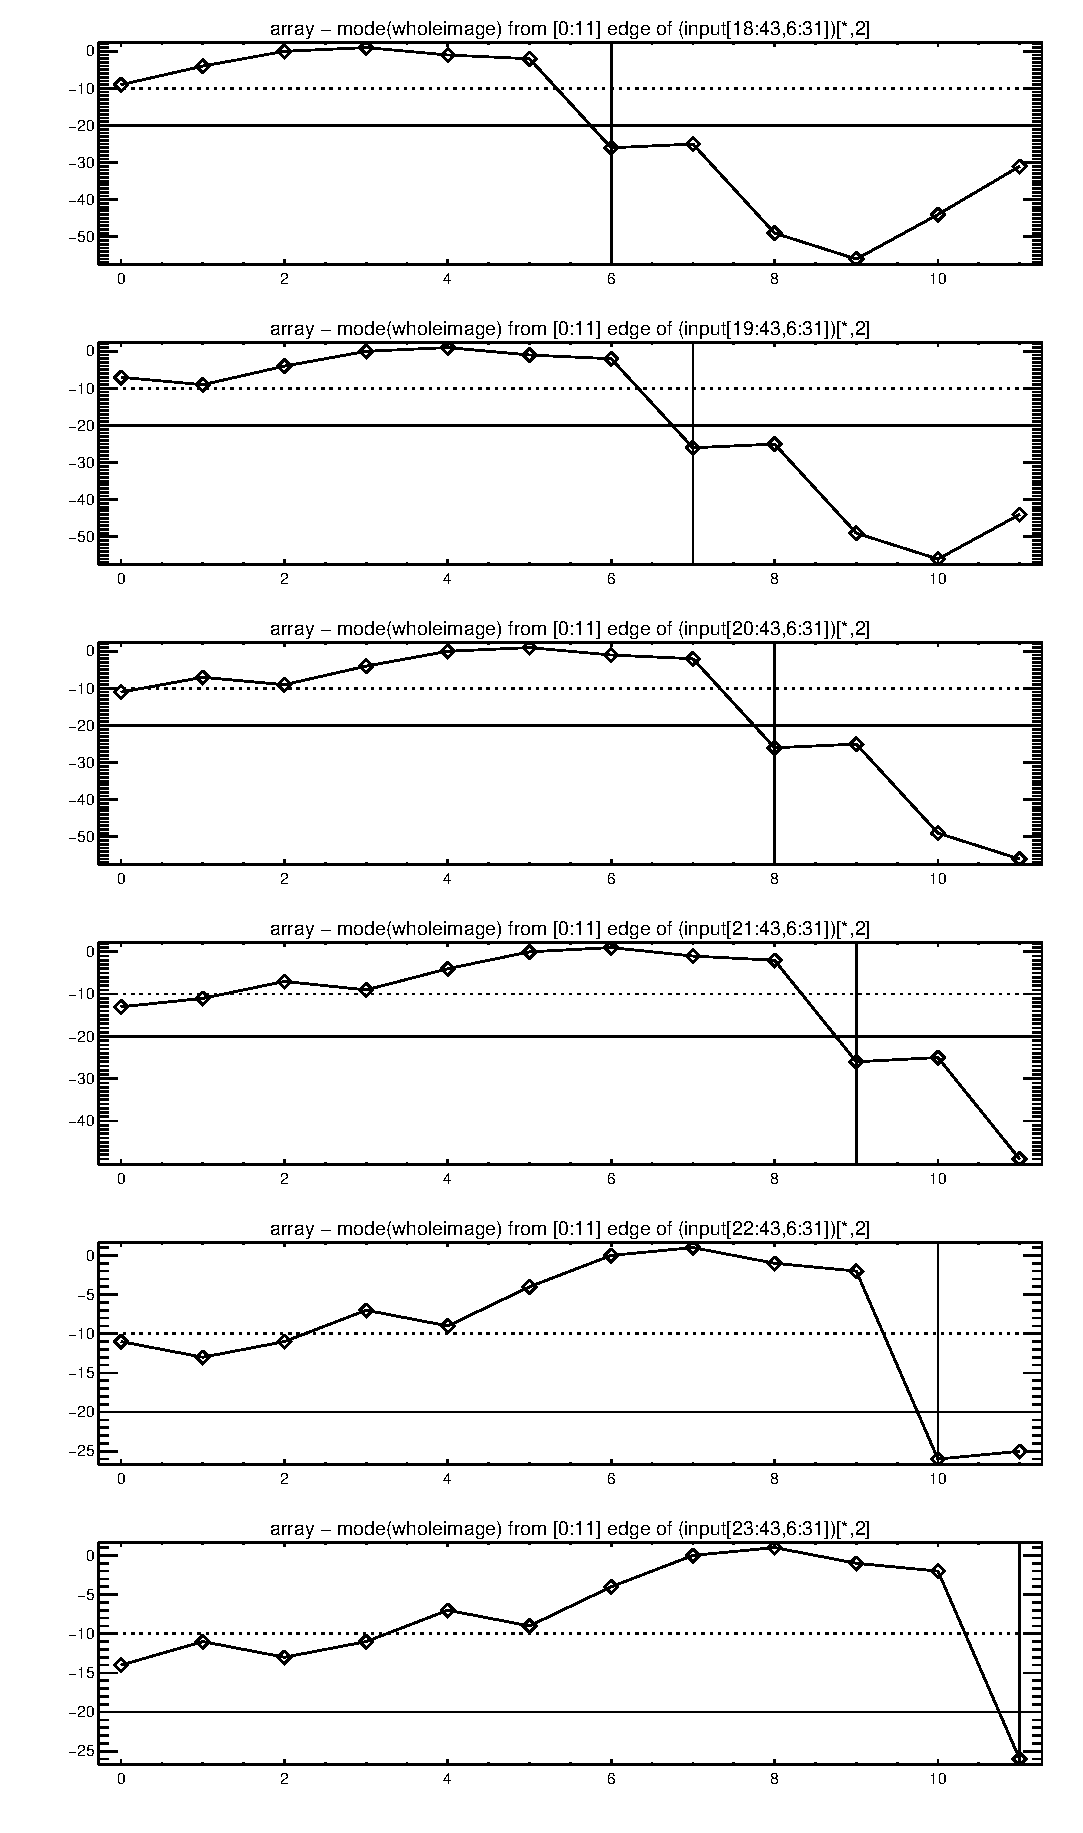
\includegraphics[width=1.4\textwidth]{../plots_tables_images/topright1.eps} 
%         \caption{Top left, left column}
%     \end{subfigure}
%     \caption{DUNNO}
% \end{figure}

% \begin{figure}[!h]
%     \centering 
%     \hspace{-1.0in}
%     \begin{subfigure}[b]{.4\linewidth}
%         \centering
%         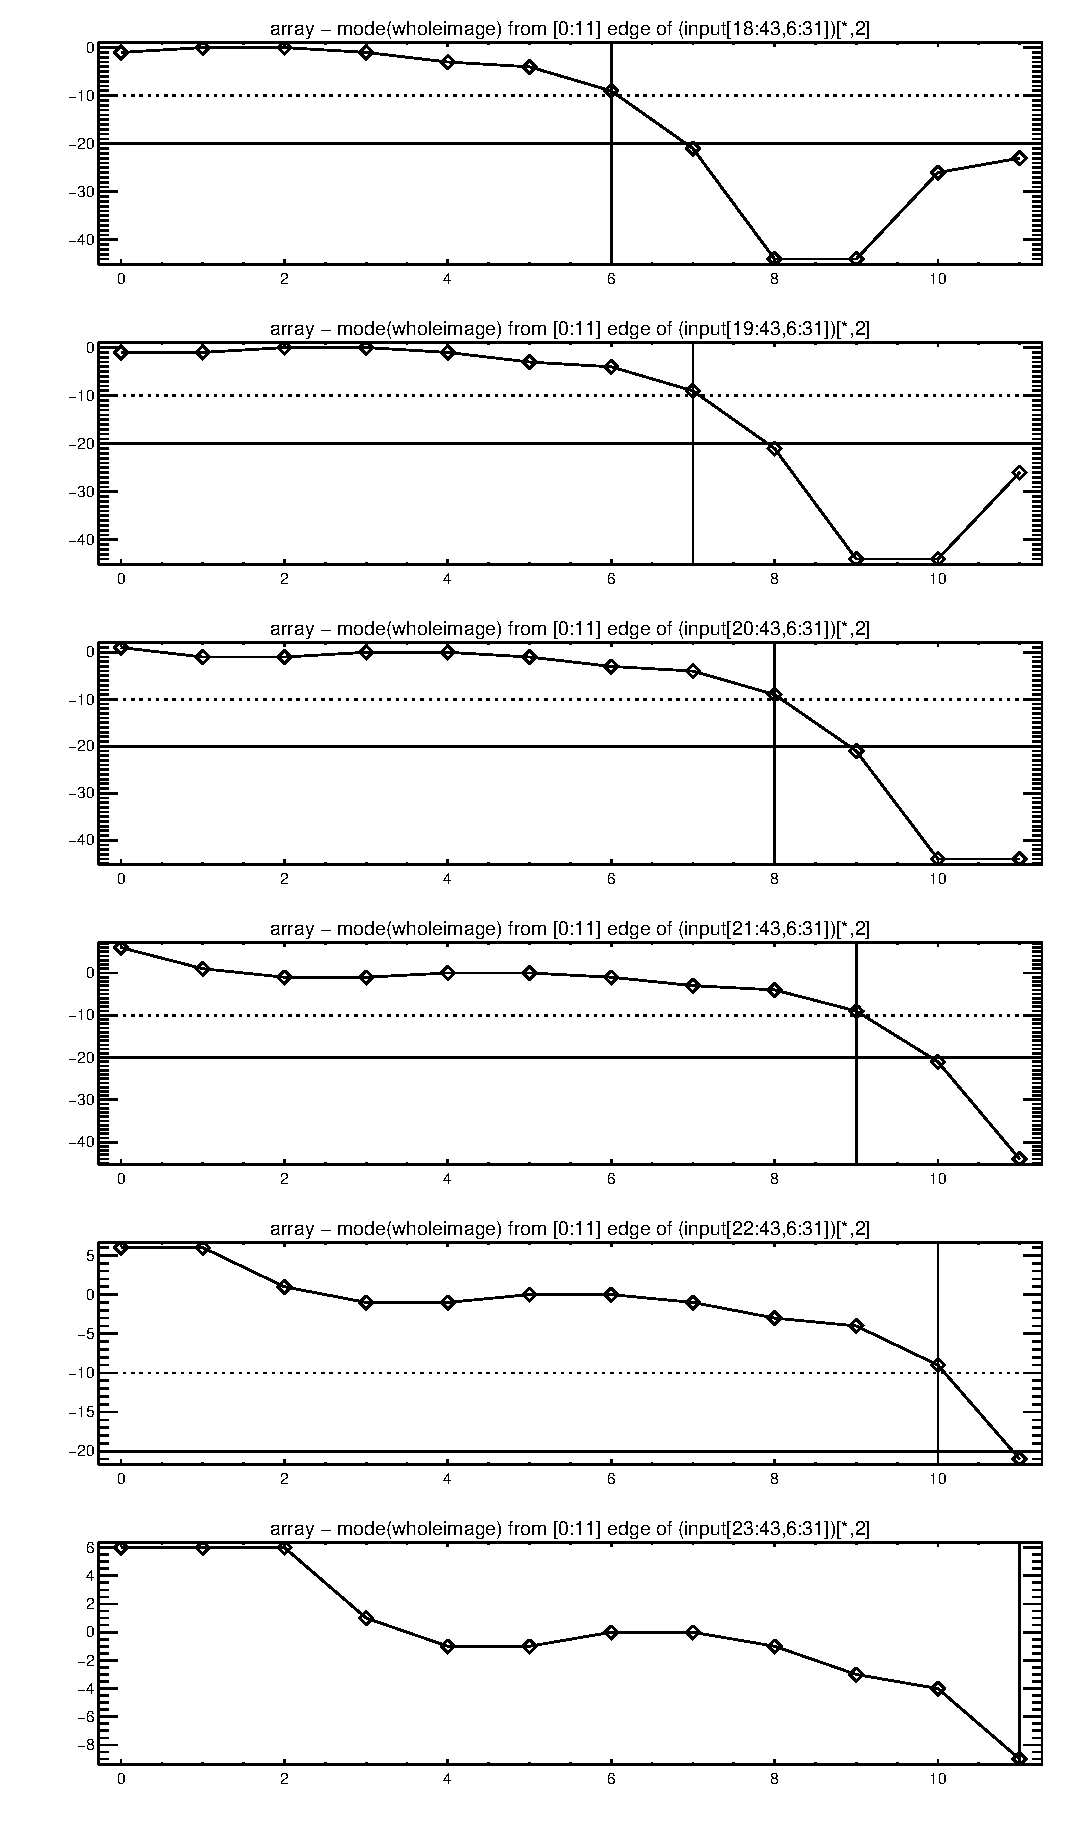
\includegraphics[width=1.4\textwidth]{../plots_tables_images/topright2.eps} 
%         \caption{Top left, top row}
%     \end{subfigure}
%     \hspace{1.0in}
%     \begin{subfigure}[b]{.4\linewidth}
%         \centering
%         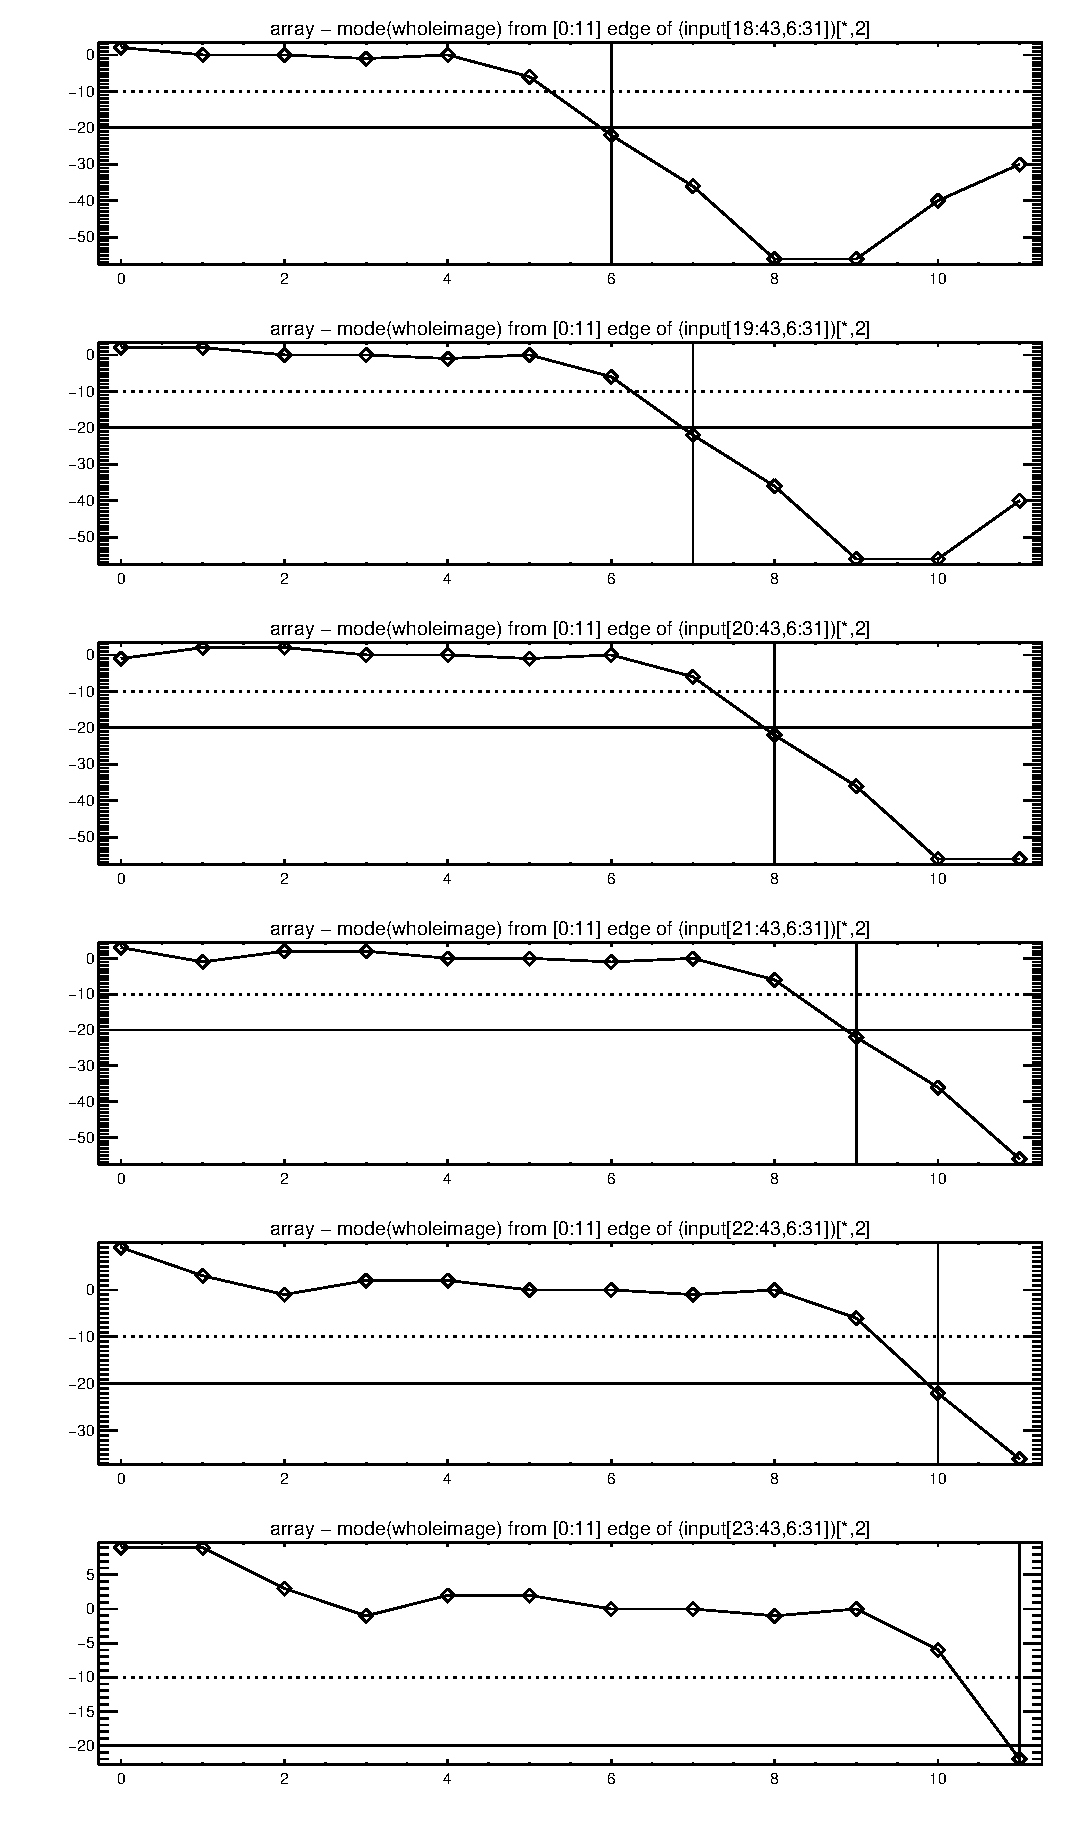
\includegraphics[width=1.4\textwidth]{../plots_tables_images/topright3.eps} 
%         \caption{Top left, bottom row}
%     \end{subfigure}
%     \caption{DUNNO}
% \end{figure}

% section laying_down_the_law_ (end)
\clearpage
% \newpage

\section{Conclusion} % (fold)
\label{sec:conclusion}
    
    Looking at all the plots, in order to fully capture 6 pixels of a fiducial, the threshold of \hl{\texttt{array - mode(wholearray)}} should be around -20. There are 9 cases where the threshold of -20 is appropriate, 5 cases for -10, 1 case for -30 and 1 case for -5.


% section conclusion (end)

\end{document}